% Chương 4: Triển khai và đánh giá
\chapter{TRIỂN KHAI VÀ ĐÁNH GIÁ}

\section{Phạm vi và môi trường triển khai}

\subsection{Phạm vi triển khai}

Chương này trình bày việc hiện thực hóa kiến trúc và khung quản trị ở Chương 3 thành một hệ thống hoạt động, nhằm kiểm chứng ba điều: logic phân quyền được đặc tả ở Mục 3.4 có đúng đắn và có thực sự chặn được các hành vi vi phạm; quy trình xác minh ở Mục 3.6 có phát hiện được các kịch bản gian lận trong mô hình đe dọa ở Mục 3.7; và hệ thống có hiệu năng đủ để việc xác minh trở thành thao tác thường xuyên chứ không phải ngoại lệ.

Hệ thống mô phỏng mô hình liên trường của ĐHQGHN: cơ quan quản trị quản lý sổ đăng ký tin cậy, các trường thành viên đóng vai trò bên phát hành, sinh viên là chủ thể, và bên xác minh hoạt động hoàn toàn độc lập.

Những nội dung nằm ngoài phạm vi triển khai được nêu rõ để tránh suy luận quá mức từ kết quả: tích hợp với hệ thống quản lý đào tạo thực tế; liên hợp giữa nhiều miền quản trị; sử dụng mô-đun bảo mật phần cứng để lưu khóa của cơ quan quản trị; kiểm thử tải ở quy mô sản xuất; và triển khai trên mạng chính.

\subsection{Thành phần và phiên bản}

\begin{longtable}{|p{3.4cm}|p{2.9cm}|p{7.3cm}|}
\caption{Thành phần và phiên bản của hệ thống thử nghiệm}
\label{tab:system-environment}
\\
\hline
\textbf{Thành phần} & \textbf{Phiên bản} & \textbf{Vai trò trong hệ thống} \\
\hline
\endfirsthead

\hline
\textbf{Thành phần} & \textbf{Phiên bản} & \textbf{Vai trò trong hệ thống} \\
\hline
\endhead

\hline
\endfoot

\hline
\endlastfoot

Mạng thử nghiệm Move
& Mã chuỗi 250
& Nguồn sự thật: định danh, thẩm quyền, trạng thái chứng thực \\
\hline

Trình biên dịch Move
& Phiên bản 3.x
& Biên dịch và xuất bản ba mô-đun hợp đồng \\
\hline

Node.js
& 20 LTS trở lên
& Môi trường chạy cài đặt TypeScript của tầng chỉ mục và công cụ phát triển giao diện \\
\hline

TypeScript
& 5.7
& Cài đặt thứ nhất của tầng chỉ mục, biên dịch ở chế độ kiểm kiểu nghiêm ngặt \\
\hline

Express, \texttt{pg}, \texttt{zod}
& 4.21 / 8.13 / 3.24
& Khung dịch vụ HTTP, truy cập cơ sở dữ liệu, kiểm tra lược đồ thân yêu cầu \\
\hline

Go
& 1.23
& Cài đặt thứ hai của tầng chỉ mục, dùng thư viện HTTP chuẩn \\
\hline

\texttt{pgx}, \texttt{golang-jwt}, \texttt{x/crypto}
& 5.7 / 5.2 / 0.31
& Truy cập cơ sở dữ liệu, ký phiên, hàm băm SHA-3 \\
\hline

PostgreSQL
& 16
& Tầng chỉ mục dùng chung cho cả hai cài đặt, kèm nhật ký kiểm toán \\
\hline

React, Vite, Tailwind
& 18.3 / 6.0 / 3.4
& Giao diện theo vai trò, gói phát hành 405\,KB \\
\hline

\texttt{@noble/curves}, \texttt{@noble/hashes}
& 1.9 / 1.8
& Ký Ed25519 và băm SHA3-256 phía máy khách, thay cho bộ công cụ của nền tảng \\
\hline

\texttt{@scure/bip39}
& 1.6
& Sinh và kiểm tra cụm từ ghi nhớ để khôi phục ví trên thiết bị khác \\
\hline

Web Cryptography API
& Theo trình duyệt
& Dẫn xuất khóa PBKDF2 và mã hóa AES-256-GCM cho kho khóa cục bộ \\
\hline

Indexed Database API
& Theo trình duyệt
& Lưu bản mã của kho khóa trên thiết bị người dùng \\
\hline

Dịch vụ ghim IPFS
& Giao diện HTTP
& Lưu DID Document và nội dung chứng thực ngoài chuỗi; có chế độ mô phỏng dùng cơ sở dữ liệu dùng chung \\
\hline

\end{longtable}


Hai điểm trong bảng trên khác với một triển khai thông thường và cần giải thích.

Thứ nhất, \textbf{tầng chỉ mục được hiện thực hóa hai lần bằng hai ngôn ngữ khác nhau} --- một bản TypeScript và một bản Go --- cài đặt cùng một hợp đồng giao diện trên cùng một lược đồ cơ sở dữ liệu. Lý do và giá trị kiểm chứng của quyết định này được trình bày tại Mục 4.4.

Thứ hai, \textbf{giao diện không sử dụng bộ công cụ phát triển chính thức của nền tảng chuỗi}. Toàn bộ thao tác mật mã và thao tác chuỗi phía máy khách được thực hiện bằng các thư viện mật mã độc lập. Cơ sở của quyết định này và cách nó được kiểm chứng được trình bày tại Mục 4.5.3.

\subsection{Quản lý thông số chuỗi}

Hệ thống có ba thành phần cùng cần biết địa chỉ gói hợp đồng và các thông số chuỗi: hai cài đặt của tầng chỉ mục và giao diện. Trong giai đoạn đầu, các thông số này được khai riêng trong tệp cấu hình của từng thành phần. Cách làm đó tạo ra một lớp lỗi khó chẩn đoán: khi triển khai lại hợp đồng mà cập nhật sót một tệp, hai cài đặt của tầng chỉ mục sẽ nói chuyện với hai gói hợp đồng khác nhau, và không thành phần nào báo lỗi --- mỗi bên đều hoạt động bình thường với gói mà nó biết, chỉ có kết quả là không nhất quán.

Thiết kế hiện tại đặt toàn bộ thông số chuỗi vào một tệp duy nhất ở gốc dự án, và một tập lệnh đồng bộ đẩy giá trị sang cấu hình của ba thành phần. Tập lệnh triển khai hợp đồng tự cập nhật tệp này sau khi xuất bản gói rồi gọi tập lệnh đồng bộ. Đây là một ví dụ nhỏ nhưng tiêu biểu cho một nguyên tắc chung trong hệ thống phân tán: một giá trị cần nhất quán giữa nhiều thành phần thì phải có đúng một nguồn, bởi sự nhất quán được duy trì bằng quy trình thủ công sẽ thất bại sớm hơn dự kiến.

\section{Lựa chọn nền tảng}

\subsection{Nền tảng chuỗi}

Việc lựa chọn nền tảng chuỗi ảnh hưởng tới cơ chế quản trị, độ trễ xác minh và khả năng mở rộng. Ba hướng được xem xét.

\begin{longtable}{|p{3.3cm}|p{3.3cm}|p{3.3cm}|p{3.3cm}|}
\caption{So sánh ba hướng nền tảng chuỗi cho hệ thống văn bằng số}
\label{tab:blockchain-comparison} \\
\hline
\textbf{Tiêu chí} & \textbf{Chuỗi công khai hợp đồng chung} & \textbf{Chuỗi được cấp phép} & \textbf{Chuỗi công khai máy ảo Move} \\
\hline
\endfirsthead

\hline
\textbf{Tiêu chí} & \textbf{Chuỗi công khai hợp đồng chung} & \textbf{Chuỗi được cấp phép} & \textbf{Chuỗi công khai máy ảo Move} \\
\hline
\endhead

\hline
\endfoot

\hline
\endlastfoot

Ngôn ngữ hợp đồng
& Solidity
& Go, Java, JavaScript
& Move
\\ \hline

Mô hình lập trình
& Hướng tài khoản
& Hướng tài khoản
& Hướng tài nguyên, hệ thống kiểu ngăn nhân bản và hủy ngoài ý muốn
\\ \hline

Kiểm soát truy cập giữa các mô-đun
& Theo quy ước và bộ sửa đổi do lập trình viên viết
& Theo chính sách của mạng
& Cơ chế \texttt{friend} ở tầng ngôn ngữ
\\ \hline

Thời gian xác nhận
& Khoảng 12 giây
& Dưới 1 giây
& Dưới 1 giây, nhờ thực thi song song
\\ \hline

Đọc dữ liệu không cần cấp phép
& Có
& \textbf{Không}: bên ngoài tập thành viên phải đi qua một cổng dịch vụ
& Có
\\ \hline

Chi phí ở giai đoạn thử nghiệm
& Cao và biến động theo thị trường
& Cần vận hành nút xác thực riêng
& Thấp trên mạng thử nghiệm
\\ \hline

Phù hợp cho kiểm chứng xác minh độc lập
& Có
& Không: không kiểm chứng được tính chất {``}không cần thỏa thuận trước{''}
& Có
\\ \hline

Phù hợp cho triển khai thật nhiều cơ sở
& Chi phí là rào cản
& Phù hợp nếu theo mô hình liên hợp
& Cần đánh giá lại chi phí và quản trị
\\ \hline

\end{longtable}


Hệ thống được triển khai trên một mạng thử nghiệm công khai sử dụng máy ảo Move \cite{Movement2024}, với bốn lý do.

Thứ nhất, \textbf{mô hình hướng tài nguyên của Move loại bỏ một lớp lỗi ở tầng ngôn ngữ} \cite{Blackshear2019Move}. Với bài toán quản lý quyền hạn, việc hệ thống kiểu bảo đảm các bản ghi thẩm quyền không thể bị nhân bản hoặc bị hủy ngoài ý muốn là một bảo đảm mạnh hơn so với việc phải kiểm tra điều đó bằng mã.

Thứ hai, \textbf{cơ chế \cbox{friend} cho phép thu hẹp bề mặt tấn công mà không mất tính mô-đun}. Mô-đun quản lý quyền cần thực hiện một số thao tác trên mô-đun định danh --- chẳng hạn đình chỉ định danh của một đơn vị bị xử lý --- và cơ chế này cho phép mở các hàm đó cho đúng một mô-đun gọi, thay vì phải công khai cho mọi bên.

Thứ ba, \textbf{thời gian xác nhận giao dịch ở mức dưới một giây} nhờ cơ chế thực thi song song Block-STM \cite{Gelashvili2023}, phù hợp với yêu cầu xác minh gần thời gian thực.

Thứ tư, \textbf{mạng công khai cho phép kiểm chứng đúng tính chất cần kiểm chứng}. Yêu cầu N1 ở Mục 3.1.3 là {``}tra cứu trạng thái thẩm quyền không cần tài khoản hay thỏa thuận trước{''}. Trên một mạng riêng, tính chất này không thể kiểm chứng được, bởi mọi bên truy vấn đều phải là thành viên. Đây là lý do một mạng công khai được chọn cho giai đoạn kiểm chứng khái niệm, dù một mạng liên hợp phù hợp hơn cho triển khai thật.

Lựa chọn này không mang tính khuyến nghị cho môi trường sản xuất, và cần nói rõ rằng lý do không chỉ nằm ở chi phí. Như phân tích tại Mục 2.5.4, cách giải thích hiện hành của cơ quan bảo vệ dữ liệu nghiêng về chuỗi được cấp phép thay vì chuỗi công khai không cần cấp phép, bởi trên chuỗi loại sau không xác định được ai là bên kiểm soát dữ liệu, và vì vậy không xác định được ai chịu trách nhiệm khi chủ thể dữ liệu thực hiện quyền của mình \cite{EDPB2025}. Đây là một lập luận về trách nhiệm pháp lý, không phải về kỹ thuật, và nó mạnh hơn lập luận về chi phí.

Khi mở rộng sang quy mô liên trường hoặc cấp quốc gia, mô hình liên hợp vì vậy phù hợp hơn ở cả ba phương diện: chi phí vận hành, cơ chế quản trị, và khả năng xác định bên kiểm soát dữ liệu. Nền tảng blockchain quốc gia \cite{NDAChain2025} --- vốn theo mô hình được cấp phép với tập nút xác thực được lựa chọn --- là một lựa chọn đáng xem xét đúng theo hướng này. Kiến trúc phân lớp ở Mục 3.3.3 cho phép chuyển đổi này mà không thiết kế lại khung quản trị, miễn nền tảng đích cung cấp ba tính chất đã nêu ở Mục 2.5.1.

\subsection{Lớp lưu trữ ngoài chuỗi}

Hệ thống dùng IPFS làm lớp lưu trữ cho DID Document và nội dung chứng thực \cite{Benet2014}. Cơ chế định địa chỉ theo nội dung bổ trợ trực tiếp cho mô hình neo: định danh nội dung chính là giá trị băm của nội dung, nên không thể thay nội dung mà giữ nguyên tham chiếu.

Hệ thống hỗ trợ hai chế độ. Chế độ thật dùng một dịch vụ ghim thương mại. Chế độ mô phỏng sinh định danh nội dung một cách tất định từ chính nội dung và lưu nội dung vào cơ sở dữ liệu dùng chung, phục vụ phát triển và kiểm thử tự động mà không cần phụ thuộc mạng ngoài.

Chi tiết về vị trí lưu nội dung ở chế độ mô phỏng đáng được ghi lại, vì nó là một lỗi thật có hai hệ quả cùng gốc. Ban đầu nội dung ở chế độ này được giữ trong bộ nhớ của tiến trình. Hệ quả thứ nhất: mỗi lần khởi động lại dịch vụ, toàn bộ nội dung đã ghim biến mất, nên mọi định danh đã đăng ký trước đó đều phân giải ra kết quả {``}không kiểm được tính toàn vẹn{''} --- đúng thứ mà hệ thống được xây dựng để bảo đảm. Hệ quả thứ hai, nghiêm trọng hơn về mặt kiến trúc: nội dung ghim qua cài đặt TypeScript thì cài đặt Go không thấy và ngược lại, nên hai cài đặt \emph{không} thực sự thay thế được cho nhau --- phá vỡ chính tính chất mà việc duy trì hai cài đặt nhằm bảo đảm. Chuyển kho nội dung mô phỏng vào cơ sở dữ liệu dùng chung sửa cả hai hệ quả, và như Mục 4.9 cho thấy, còn mang lại một cải thiện hiệu năng đáng kể. Bài học tổng quát: bất cứ trạng thái nào mà nhiều thành phần cùng phải thấy thì không được giữ trong bộ nhớ tiến trình.

\section{Hợp đồng thông minh}

\subsection{Ba mô-đun và quan hệ phụ thuộc}

Hệ thống triển khai ba mô-đun theo nguyên tắc phân tách trách nhiệm, cùng hai mô-đun tiện ích chứa hằng số và mã lỗi dùng chung.

\begin{itemize}
    \item \cbox{did\_registry} quản lý định danh và DID Document: đăng ký, cập nhật kèm số phiên bản, đình chỉ, kích hoạt lại, thu hồi, và cung cấp các hàm phân giải. Mô-đun này không phụ thuộc hai mô-đun còn lại.
    \item \cbox{authority} quản lý chuỗi thẩm quyền: quản trị viên gốc, quản trị viên, bên phát hành, chuyển quyền gốc hai bước, và các thao tác quản trị trên định danh. Mô-đun này phụ thuộc \cbox{did\_registry}, bởi một thực thể phải có định danh đang hoạt động mới được cấp thẩm quyền.
    \item \cbox{vc\_registry} quản lý bản ghi neo và trạng thái của chứng thực. Mô-đun này phụ thuộc cả hai mô-đun trên: trước khi ghi một bản ghi chứng thực, nó kiểm thẩm quyền của bên phát hành qua \cbox{authority} và kiểm trạng thái định danh của cả bên phát hành lẫn chủ thể qua \cbox{did\_registry}.
\end{itemize}

Quan hệ phụ thuộc là một chiều, nhất quán với Nguyên tắc 2 ở Mục 3.2. Các hàm nội bộ mà \cbox{authority} cần gọi trên \cbox{did\_registry} được khai báo qua cơ chế \cbox{friend}, nên chúng không thuộc giao diện công khai của hợp đồng.

Một chi tiết thiết kế trong hàm cấp phát chứng thực đáng được nêu: định danh của bên phát hành \emph{không} được nhận từ tham số đầu vào mà được suy ra từ địa chỉ của người ký giao dịch, thông qua một hàm tra cứu định danh đang hoạt động của địa chỉ đó. Nếu nhận từ tham số, một bên phát hành hợp lệ có thể khai định danh của một trường khác và tạo ra chứng thực mang tên trường đó --- một dạng mạo danh mà mọi phép kiểm tra chữ ký vẫn cho kết quả đạt.

\subsection{Mô hình dữ liệu trên chuỗi}

Bản ghi thẩm quyền --- thành phần trung tâm của khung quản trị --- có cấu trúc như sau:

\lstinputlisting[
    language=Move,
    caption={Cấu trúc bản ghi thẩm quyền trong mô-đun \texttt{authority}}
]{source/code/issuer-record.move}

Bốn trường trong cấu trúc này hiện thực hóa trực tiếp các nội dung thiết kế ở Mục 3.4. Trường \cbox{vc\_type\_mask} là mặt nạ bit biểu diễn phạm vi cấp phát (Mục 3.4.2). Trường \cbox{expires\_at} là thời hạn ủy quyền, với giá trị không tương ứng với ủy quyền vô thời hạn. Hai trường \cbox{delegation\_vc\_cid} và \cbox{delegation\_vc\_hash} lưu tham chiếu tới chứng thực ủy quyền (Mục 3.4.3). Trường \cbox{version} hiện thực hóa cơ chế khôi phục vai trò mà vẫn giữ dấu vết kiểm toán (Mục 3.4.6): khi một đơn vị bị thu hồi rồi được cấp lại, bản ghi mới có số phiên bản tăng thêm một, còn bản ghi cũ vẫn nằm trong tập bản ghi.

Cấu trúc bản ghi định danh và bản ghi chứng thực theo nguyên tắc tương tự. Bản ghi định danh lưu chuỗi định danh, định danh nội dung và giá trị băm của DID Document, trạng thái, số phiên bản, cùng một trường ghi lại \emph{ai} đã đặt trạng thái đình chỉ --- trường cuối cần thiết để phân biệt trường hợp chủ thể tự đình chỉ với trường hợp bị quản trị viên đình chỉ, theo quy định ở Bảng \ref{tab:role-permission}. Bản ghi chứng thực lưu giá trị băm của định danh chứng thực, định danh nội dung và giá trị băm của nội dung, loại văn bằng, trạng thái, thời điểm cấp và thời điểm hết hạn.

Một quyết định về bộ đếm cần được nêu, vì nó ảnh hưởng tới số liệu mà giao diện hiển thị. Hệ thống duy trì hai nhóm bộ đếm cho mỗi bên phát hành và mỗi chủ thể: \emph{tổng số đã từng cấp}, chỉ tăng và không bao giờ giảm, phục vụ mục đích thống kê; và \emph{số đang có hiệu lực}, giảm khi chứng thực bị thu hồi hoặc bị đình chỉ và tăng lại khi được kích hoạt. Nếu chỉ có nhóm thứ nhất, con số {``}số văn bằng{''} hiển thị trên giao diện sẽ bao gồm cả những văn bằng đã bị thu hồi.

\subsection{Phương thức định danh và mẫu dữ liệu}

Phương thức \cbox{did:vnu} được hiện thực theo đặc tả ở Mục 3.5.3. Dưới đây là một DID Document của bên phát hành như hệ thống thực sự sinh ra:

\lstinputlisting[
    language=json,
    caption={DID Document của một bên phát hành}
]{source/json/issuer-uet.json}

Cấu trúc này gọn hơn so với một số triển khai khác và sự gọn nhẹ là có chủ đích. Khóa công khai được biểu diễn ở dạng thập lục phân thay vì dạng đa cơ số, để cùng một giá trị dùng được trực tiếp cho cả việc kiểm tra chữ ký chứng thực và việc kiểm tra chữ ký giao dịch mà không cần bước chuyển đổi. Hai trường \cbox{authentication} và \cbox{assertionMethod} được khai riêng theo đặc tả, dù trong bản thử nghiệm chúng trỏ tới cùng một khóa; việc giữ hai trường riêng là để khi tách khóa đăng nhập và khóa cấp phát --- điều cần thiết trong triển khai thật --- không phải thay đổi cấu trúc tài liệu.

Và đây là một chứng thực văn bằng:

\lstinputlisting[
    language=json,
    caption={Chứng thực văn bằng do bên phát hành sinh ra}
]{source/json/VC-example.json}

Ba điểm về cấu trúc này cần được nêu tường minh, bao gồm cả những điểm chưa tuân thủ đầy đủ chuẩn.

Thứ nhất, \textbf{các thuộc tính riêng của hệ thống được đặt trong một không gian tên riêng} khai báo qua \cbox{@context}, thay vì đặt trực tiếp ở mức gốc. Cách này bảo đảm một bên xử lý JSON-LD không nhầm các thuộc tính riêng với thuộc tính của chuẩn.

Thứ hai, \textbf{bản thử nghiệm dùng ngữ cảnh của mô hình dữ liệu chứng thực phiên bản 1.1 thay vì phiên bản 2.0}. Đây là một điểm chưa tuân thủ phiên bản chuẩn mới nhất \cite{W3C_VCDM2025} và được ghi nhận như một hạn chế.

Thứ ba, \textbf{bằng chứng được lưu tách rời thay vì nhúng trong tài liệu}. Giá trị chữ ký được lưu trong tầng chỉ mục và trong bản trình bày chứ không nằm trong đối tượng chứng thực được ghim. Lý do kỹ thuật: giá trị băm neo trên chuỗi được tính trên chính đối tượng chứng thực, nên nếu nhúng chữ ký vào đối tượng thì phải định nghĩa thêm quy tắc loại trừ trường bằng chứng khi băm. Cách tách rời đơn giản hơn nhưng khác với cấu trúc mà một bên xác minh theo chuẩn mong đợi, nên là một hạn chế về khả năng liên thông.

Thứ tư, \textbf{trường trạng thái không theo cơ chế danh sách bit của chuẩn} \cite{W3C_BitstringStatusList2025} mà trỏ tới hợp đồng trên chuỗi, theo đánh đổi đã phân tích ở Mục 3.8. Bên xác minh dùng giá trị băm của định danh chứng thực làm khóa để tra cứu, và kết quả trả về gồm cả trạng thái lẫn giá trị băm của nội dung --- nhờ đó một lần truy vấn phục vụ được cả bước thứ năm và bước thứ sáu của quy trình xác minh.

\subsection{Mã lỗi và thông điệp}

Hợp đồng định nghĩa một tập mã lỗi riêng cho từng loại vi phạm, chia theo nhóm tương ứng ba mô-đun: nhóm thẩm quyền (không phải quản trị viên gốc, không phải quản trị viên, bên phát hành không hoạt động, thẩm quyền đã hết hạn, loại văn bằng không được phép, xung đột vai trò, không được ủy quyền lại), nhóm định danh (định danh đã tồn tại, không tìm thấy, không hoạt động, địa chỉ đã có định danh, định danh nội dung không hợp lệ) và nhóm chứng thực (không tìm thấy, không hoạt động, đã thu hồi, đã hết hạn, không phải bên cấp, đã tồn tại). Ngoài ra có nhóm mã lỗi chung cho sai độ dài giá trị băm, giá trị băm không khớp và vượt giới hạn kết quả.

Việc tách mã lỗi chi tiết thay vì dùng một mã chung có một giá trị cụ thể trong kiểm thử, liên quan tới nhận định ở Mục 1.5.2. Một phép kiểm trường hợp vi phạm chỉ có giá trị nếu nó thất bại \emph{vì đúng nguyên nhân dự kiến}. Nếu hợp đồng chỉ trả một mã lỗi chung, không thể phân biệt trường hợp {``}phép kiểm thẩm quyền đã chặn{''} với trường hợp {``}một phép kiểm định dạng nào đó chặn trước, chưa chạm tới phép kiểm thẩm quyền{''}. Tình huống thứ hai đã thực sự xảy ra trong quá trình phát triển: một phép kiểm về việc từ chối mã giao dịch bịa đặt cho kết quả đạt, nhưng nguyên nhân thật là một định danh nội dung sai định dạng đã bị chặn trước đó, nên bước xác minh giao dịch chưa từng được thực thi. Mã lỗi chi tiết cho phép phép kiểm khẳng định đúng nguyên nhân.

Ở tầng giao diện, mỗi mã lỗi được chuyển thành một câu tiếng Việt nêu rõ nguyên nhân và hành động cần làm, thay vì hiển thị mã số. Đây không chỉ là vấn đề trải nghiệm: một thông điệp nêu đúng nguyên nhân giúp người dùng phân biệt được {``}tôi không có quyền{''} với {``}thẩm quyền của tôi đã hết hạn{''} --- hai tình huống cần hai cách xử lý khác nhau.

\subsection{Rà soát an toàn hợp đồng và kết quả xử lý}

Hợp đồng đã trải qua một đợt rà soát an toàn có hệ thống, trong đó mỗi vấn đề phát hiện được chứng minh bằng một phép kiểm thể hiện hệ quả của nó trước khi sửa. Mười vấn đề được xác nhận là lỗi thật.

\begin{longtable}{|c|p{4.1cm}|p{8.3cm}|}
\caption{Mười vấn đề phát hiện trong đợt rà soát an toàn hợp đồng và cách xử lý}
\label{tab:contract-audit} \\

\hline
\textbf{Mã} & \textbf{Vấn đề} & \textbf{Cách xử lý} \\
\hline
\endfirsthead

\hline
\textbf{Mã} & \textbf{Vấn đề} & \textbf{Cách xử lý} \\
\hline
\endhead

\hline
\endfoot

\hline
\endlastfoot

V1 & Chuyển quyền gốc một bước, không kiểm tra được địa chỉ đích có người kiểm soát
& Thay bằng cơ chế hai bước: đề cử rồi ký nhận, kèm thao tác hủy đề cử. Hàm chuyển một bước bị xóa. Hàm khởi tạo tự lấy người xuất bản làm quản trị viên gốc khi không được truyền tham số
\\ \hline

V2 & Mọi bên phát hành đều bị đòi giá trị băm chứng thực ủy quyền, kể cả bên không có quan hệ ủy quyền nào
& Phép kiểm độ dài giá trị băm chuyển vào trong nhánh điều kiện; chỉ bắt buộc khi thực sự có quan hệ ủy quyền. Giá trị rỗng được chấp nhận, nhưng giá trị sai độ dài vẫn bị từ chối
\\ \hline

V3 & Không có cơ chế ủy quyền nhiều cấp
& Bên phát hành có bit ủy quyền phê duyệt được bên phát hành cấp dưới, với ba ràng buộc: phạm vi là tập con, thời hạn không vượt thời hạn cha, bit ủy quyền không truyền tiếp
\\ \hline

V4 & Quản trị viên và bên phát hành bị thu hồi không thể được cấp lại
& Cho phép cấp lại; bản ghi mới có số phiên bản tăng thêm một, bản ghi cũ giữ nguyên trong tập bản ghi làm dấu vết kiểm toán
\\ \hline

V5 & Định danh bị thu hồi khóa địa chỉ vĩnh viễn, nên lộ khóa riêng đồng nghĩa mất địa chỉ
& Cho phép đăng ký định danh mới sau khi định danh cũ đã bị thu hồi; định danh cũ vẫn tra cứu ra trạng thái đã thu hồi
\\ \hline

V6 & Định danh nội dung không được kiểm tra độ dài, dù trong mã có chú thích nói rằng có kiểm
& Bổ sung phép kiểm ở cả ba thao tác: đăng ký định danh, cập nhật tài liệu định danh và cấp phát chứng thực
\\ \hline

V7 & Không phân biệt được chủ thể tự đình chỉ định danh với bị quản trị viên đình chỉ
& Bổ sung các thao tác tự đình chỉ và tự kích hoạt lại, cùng một trường ghi lại ai đã đặt trạng thái đình chỉ: tự khóa thì tự mở, bị quản trị viên khóa thì phải quản trị viên mở
\\ \hline

V8 & Thu hồi chứng thực đòi hỏi thẩm quyền còn hiệu lực, nên đơn vị hết hạn ủy quyền không thu hồi được văn bằng mình đã cấp
& Thu hồi chỉ cần quyền sở hữu và định danh còn hoạt động; bỏ phép kiểm thẩm quyền còn hiệu lực
\\ \hline

V9 & Tham số thời hạn của chứng thực bị ghi cứng bằng giá trị không, khiến toàn bộ nhánh xử lý hết hạn là mã chết
& Thời hạn trở thành tham số thật, với giá trị không tương ứng vĩnh viễn; hàm tra cứu chứng thực không còn dừng đột ngột mà trả về bản ghi kèm trạng thái đã tính
\\ \hline

V10 & Các hàm truy vấn liệt kê toàn bộ danh sách sẽ vỡ âm thầm khi vượt giới hạn chi phí tính toán
& Bổ sung các hàm truy vấn phân trang; các hàm liệt kê toàn bộ dừng rõ ràng khi vượt ngưỡng an toàn thay vì vỡ âm thầm
\\ \hline

V11 & Nhóm vấn đề nhỏ: mã lỗi không khớp loại vi phạm, nhánh mã không bao giờ thực thi, bộ sinh số hiệu vai trò có thể trùng, một địa chỉ giữ đồng thời hai vai trò xung đột, bộ đếm không phân biệt tổng đã cấp và số đang hiệu lực
& Xử lý từng mục: đúng mã lỗi, bỏ nhánh chết, tách bộ sinh số hiệu riêng chỉ tăng, chặn xung đột vai trò, bổ sung nhóm bộ đếm số chứng thực đang hiệu lực
\\ \hline

\end{longtable}


Ba vấn đề trong bảng trên đã trở thành nguyên tắc thiết kế được trình bày ở Chương 3, và quá trình phát hiện chúng minh họa giá trị của việc rà soát: cả ba đều không phải lỗi lập trình mà là lỗi mô hình.

Vấn đề thứ nhất là cơ chế chuyển quyền gốc một bước, dẫn tới nguyên tắc ở Mục 3.4.4. Phép kiểm cho thấy hệ quả: sau khi chuyển quyền tới một địa chỉ không ai kiểm soát, hệ thống vẫn chạy bình thường nhưng toàn bộ năng lực quản trị mất vĩnh viễn.

Vấn đề thứ hai là việc thu hồi chứng thực đòi hỏi thẩm quyền còn hiệu lực, dẫn tới nguyên tắc bất đối xứng ở Mục 3.4.5. Phép kiểm dựng đúng kịch bản đã phân tích: một đơn vị hết hạn ủy quyền phát hiện gian lận trong văn bằng mình đã cấp và không thu hồi được.

Vấn đề thứ ba là việc một định danh bị thu hồi khóa địa chỉ vĩnh viễn, dẫn tới cơ chế phiên bản ở Mục 3.4.6. Kịch bản thật là lộ khóa riêng: hành động đúng của người dùng là thu hồi định danh cũ và đăng ký định danh mới bằng khóa mới, nhưng thiết kế ban đầu khiến hành động đó làm mất địa chỉ.

Một vấn đề khác đáng nêu vì nó thuộc loại lỗi khó phát hiện nhất --- mã chết tạo cảm giác an toàn giả. Tham số thời hạn của chứng thực ban đầu bị ghi cứng bằng giá trị không, nên toàn bộ nhánh xử lý hết hạn là mã không bao giờ được thực thi: trạng thái {``}đã hết hạn{''} không bao giờ được ghi, và hai phép kiểm chặn nó không bao giờ đúng. Mã nguồn trông như đã xử lý việc hết hạn, trong khi thực tế không. Đây là trường hợp cụ thể của nhận định ở Mục 1.5.2: một bước kiểm tra luôn cho kết quả đạt còn tệ hơn việc không có bước đó.

Sau khi xử lý toàn bộ mười vấn đề, bộ kiểm thử được viết lại theo một tiêu chí khác. Trước đó, mỗi phép kiểm đạt nghĩa là lỗi \emph{có thật}; sau khi sửa, mỗi phép kiểm đạt nghĩa là lỗi \emph{đã được sửa và không quay lại}. Quy mô bộ kiểm thử tăng từ 94 lên 126 phép.

\section{Tầng chỉ mục với hai cài đặt độc lập}

\subsection{Lý do duy trì hai cài đặt}

Tầng chỉ mục được hiện thực hóa hai lần: một bản bằng TypeScript trên Express và một bản bằng Go trên thư viện HTTP chuẩn, cùng cài đặt một hợp đồng giao diện trên cùng một lược đồ cơ sở dữ liệu. Giao diện người dùng chọn cài đặt nào để làm việc ngay lúc chạy, và vì hai bản dùng chung khóa ký phiên, một phiên đăng nhập do bên này cấp dùng được ở bên kia.

Mục đích của việc này không phải dự phòng mà là \textbf{biến đặc tả giao diện từ một tài liệu thành một tính chất kiểm chứng được}. Khi chỉ có một cài đặt, đặc tả giao diện là những gì mã nguồn làm --- không có cách nào phát hiện rằng một hành vi là quyết định thiết kế hay là hệ quả tình cờ của thư viện được dùng. Khi có hai cài đặt độc lập cùng một bộ đối chiếu, mọi điểm khác biệt giữa chúng đều lộ ra, và mỗi điểm khác biệt buộc phải được giải quyết thành một quyết định tường minh.

Cách làm này đã phát hiện ba loại lệch mà một bộ kiểm thử thông thường không bắt được.

\textbf{Lệch về xử lý trường lạ trong thân yêu cầu.} Thư viện kiểm tra lược đồ bên TypeScript mặc định \emph{bỏ qua} các trường không khai báo, trong khi bộ giải mã JSON chuẩn của Go \emph{từ chối} chúng. Cùng một yêu cầu cho hai mã trạng thái khác nhau. Điểm lệch này ẩn rất lâu vì luồng sử dụng bình thường không gửi trường lạ; nó chỉ lộ ra khi một kịch bản kiểm thử vô tình gửi thừa một trường. Hướng xử lý đã chọn là nghiêm ngặt ở cả hai bên, với lý do cụ thể: gõ nhầm tên trường thời hạn phải báo lỗi ngay, chứ không được âm thầm cấp một văn bằng vô thời hạn.

\textbf{Lệch về thứ tự kiểm tra đầu vào.} Bản TypeScript kiểm {``}định danh đã tồn tại{''} trước, bản Go kiểm độ dài giá trị băm trước. Cùng một yêu cầu sai cho hai mã lỗi khác nhau. Điểm lệch này ẩn vì ở chế độ nghiêm ngặt, cả hai bên đều dừng sớm hơn ở bước xác minh giao dịch. Hướng xử lý: cả hai theo thứ tự rẻ trước, đắt sau --- kiểm định dạng trong bộ nhớ, rồi truy vấn cơ sở dữ liệu, rồi gọi nút đầy đủ. Nhận định rút ra là \textbf{thứ tự kiểm tra đầu vào cũng là một phần của hợp đồng giao diện}, không phải chi tiết triển khai.

\textbf{Lệch về tuyến không được cài đặt.} Hai tuyến đọc chi tiết một chứng thực chỉ tồn tại ở bản TypeScript; bản Go không đăng ký tuyến nào cho chúng. Bộ đối chiếu vẫn cho kết quả đạt toàn bộ trong thời gian dài vì không phép đối chiếu nào chạm tới hai tuyến đó. Điểm lệch chỉ lộ ra khi màn hình quản trị cần đọc số hiệu trên chuỗi của một văn bằng. Nhận định rút ra: \textbf{một bộ đối chiếu chỉ kiểm được những gì nó biết}, nên việc thêm tuyến mới phải kéo theo việc thêm phép đối chiếu ngay tại thời điểm đó.

\subsection{Ba bất biến phải giữ giữa các cài đặt}

Ba tính chất sau phải giống nhau từng byte ở cả ba nơi --- hai cài đặt tầng chỉ mục và giao diện --- và mỗi tính chất có bộ kiểm riêng.

\textbf{Thứ nhất, chuỗi được ký khi đăng nhập.} Cơ chế đăng nhập theo thách thức -- đáp ứng: dịch vụ sinh một số dùng một lần, giao diện dựng một thông điệp theo khuôn cố định chứa địa chỉ và số đó rồi ký, dịch vụ kiểm chữ ký bằng khóa công khai đã ghi danh. Không mật khẩu nào đi qua mạng. Nếu khuôn thông điệp lệch một ký tự giữa giao diện và dịch vụ, chữ ký sẽ không bao giờ khớp.

\textbf{Thứ hai, phép tuần tự hóa tất định.} Khóa đối tượng sắp xếp tăng dần, không khoảng trắng dư, số nguyên biểu diễn không có phần thập phân. Đây là đầu vào của mọi phép băm, nên một khác biệt nhỏ ở đây làm toàn bộ bước kiểm tra toàn vẹn thất bại trong khi dữ liệu hoàn toàn nguyên vẹn.

\textbf{Thứ ba, hàm băm.} SHA3-256 trên bản tuần tự hóa tất định, trả về tiền tố \cbox{0x} cùng 64 ký tự thập lục phân. Ba cài đặt dùng ba thư viện khác nhau --- thư viện mật mã chuẩn của môi trường chạy JavaScript, một thư viện mật mã độc lập ở giao diện, và thư viện mật mã mở rộng của Go --- và đã được đối chiếu cho cùng kết quả, bao gồm các trường hợp có ký tự tiếng Việt và cấu trúc lồng sâu.

\subsection{Xác minh giao dịch trước khi ghi chỉ mục}

Theo Nguyên tắc 3 ở Mục 3.2, cơ sở dữ liệu chỉ là chỉ mục và chuỗi là nguồn sự thật. Hệ quả là mọi bản ghi chỉ mục có tham chiếu trên chuỗi đều mang một mã giao dịch, và tầng dịch vụ kiểm bốn điều với nút đầy đủ trước khi ghi:

\begin{enumerate}
    \item Giao dịch \textbf{tồn tại} trên chuỗi.
    \item Giao dịch \textbf{thành công}.
    \item Hàm được gọi trong phần tải của giao dịch \textbf{đúng là hàm mong đợi} của tuyến đó.
    \item Người gửi giao dịch \textbf{khớp} tài khoản đang thực hiện yêu cầu, sau khi chuẩn hóa địa chỉ.
\end{enumerate}

Bốn phép kiểm này là rào chắn cho các hành vi T4, T5 và T6 trong mô hình đe dọa. Vai trò của từng phép kiểm đã được phân tích ở Mục 3.7.2; điểm cần nhấn mạnh là \emph{không} phép kiểm nào trong bốn phép này là dư thừa: thiếu phép kiểm thứ ba, kẻ tấn công tái sử dụng được một giao dịch thật của mình nhưng thuộc loại thao tác khác; thiếu phép kiểm thứ tư, họ tái sử dụng được giao dịch của người khác.

Việc so khớp tên hàm ở phép kiểm thứ ba dẫn tới một yêu cầu kỹ thuật: tên hàm hợp đồng xuất hiện ở ba nơi --- mã Move, hai cài đặt tầng chỉ mục, và tầng chuỗi của giao diện. Một sai lệch giữa các nơi này tạo ra kiểu hỏng khó chẩn đoán nhất: giao dịch lên chuỗi thành công nhưng tầng dịch vụ từ chối ghi chỉ mục, nên hệ thống hỏng đúng nửa chừng. Một bộ kiểm đọc trực tiếp mã Move, rút ra tập hàm công khai rồi đối chiếu với tên mà từng thành phần đang dùng, được bổ sung đúng để chặn lớp lỗi này. Khi bộ kiểm được mở rộng từ hai nơi lên ba nơi, nó phát hiện ngay một sai lệch thật: giao diện gọi thao tác đình chỉ chứng thực bằng một tên, trong khi tầng dịch vụ xác minh giao dịch đình chỉ bằng một tên khác.

\subsection{Chế độ không phụ thuộc chuỗi và các rào chắn đi kèm}

Hệ thống có một cờ chế độ cho phép chạy và kiểm thử khi chưa có chuỗi hoặc khi chuỗi được dựng lại. Thiết kế của cờ này đáng được trình bày, vì phiên bản đầu của nó là một ví dụ về việc một cờ chế độ nửa vời còn tệ hơn không có cờ.

Ban đầu, cờ chỉ bỏ qua bước xác minh giao dịch mà \emph{không} bỏ qua việc kiểm quyền trên chuỗi. Kết quả là hệ thống vẫn không chạy được khi chưa có chuỗi, vì mọi câu hỏi về quyền hạn và trạng thái đều phải gọi tới hợp đồng. Cờ không đạt được mục đích của chính nó. Thiết kế hiện tại áp dụng cờ nhất quán trên toàn bộ các đường phụ thuộc: khi tắt, cả hai cài đặt bỏ qua xác minh giao dịch \emph{và} trả lời các câu hỏi về quyền, định danh, trạng thái chứng thực bằng chỉ mục cơ sở dữ liệu thay vì bằng hàm truy vấn trên chuỗi.

Điểm thiết kế quan trọng là chế độ này \emph{không} trả kết quả chấp nhận vô điều kiện. Một chủ thể vẫn bị chặn khỏi các tuyến của bên phát hành, một bên tự khai là bên phát hành vẫn bị từ chối. Nếu trả kết quả chấp nhận vô điều kiện, bộ kiểm thử chạy ở chế độ này sẽ không chứng minh được điều gì về logic phân quyền --- nó chỉ chứng minh rằng hệ thống không báo lỗi.

Bốn rào chắn đi kèm để cờ này không trở thành một lỗ hổng:

\begin{itemize}
    \item Khởi động ở môi trường sản xuất cùng với cờ này ở trạng thái tắt sẽ làm tiến trình thoát ngay, ở cả hai cài đặt.
    \item Tuyến kiểm tra trạng thái dịch vụ trả về giá trị của cờ, và giao diện hiển thị một dải cảnh báo rõ ràng.
    \item Nguồn dữ liệu trong mỗi phản hồi được báo đúng là chỉ mục cơ sở dữ liệu, không khai là chuỗi.
    \item Một bộ kiểm riêng chứng minh rằng ở chế độ nghiêm ngặt, hệ thống vẫn chặn mã giao dịch bịa đặt và vẫn từ chối bên tự khai là bên phát hành.
\end{itemize}

Rào chắn thứ ba đáng được nhấn mạnh. Trong một hệ thống mà giá trị cốt lõi là tính kiểm chứng được, việc báo sai nguồn dữ liệu nghiêm trọng hơn việc không có dữ liệu: người dùng tin rằng một tuyên bố đã được chuỗi xác nhận trong khi nó chỉ đến từ một chỉ mục có thể bị sửa.

\subsection{Nhật ký kiểm toán}

Yêu cầu F12 đòi hỏi mọi thao tác thay đổi trạng thái đều để lại dấu vết. Hiện thực hóa yêu cầu này có một chi tiết đáng ghi lại: bảng nhật ký kiểm toán tồn tại trong lược đồ cơ sở dữ liệu từ đầu, nhưng \emph{không cài đặt nào ghi vào đó}, nên tuyến đọc nhật ký luôn trả về rỗng. Không bộ kiểm thử nào phát hiện điều này, vì không bộ nào kiểm nội dung của nhật ký --- chúng chỉ kiểm rằng tuyến trả về đúng định dạng.

Hiện tại cả hai cài đặt cùng ghi nhật ký với cùng một bộ tên hành động, và bộ kiểm thử kiểm nội dung thực của nhật ký sau mỗi thao tác. Việc ghi nhật ký thất bại chỉ sinh một dòng lỗi và không làm thất bại thao tác chính --- nhật ký là dữ liệu phụ trợ, không được phép làm hỏng thao tác nghiệp vụ.

Nhận định rút ra có giá trị tổng quát: \textbf{một bảng có sẵn trong lược đồ không có nghĩa là có thành phần nào ghi vào nó}, và một tuyến trả về đúng định dạng không có nghĩa là nó trả về đúng dữ liệu.

\section{Ví định danh và tầng chuỗi phía máy khách}

\subsection{Mô hình bảo vệ khóa}

Ví được hiện thực theo mô hình không lưu ký đã chọn ở Mục 3.8. Khóa riêng được sinh và lưu hoàn toàn phía máy khách; tầng dịch vụ không lưu và không có khả năng truy cập khóa riêng dưới bất kỳ hình thức nào.

\begin{longtable}{|p{3.1cm}|p{10.6cm}|}
\caption{Mô hình bảo vệ khóa của ví không lưu ký}
\label{tab:wallet-security} \\

\hline
\textbf{Lớp bảo vệ} & \textbf{Cách thực hiện} \\
\hline
\endfirsthead

\hline
\textbf{Lớp bảo vệ} & \textbf{Cách thực hiện} \\
\hline
\endhead

\hline
\endfoot

\hline
\endlastfoot

Sinh khóa
& Cặp khóa Ed25519 sinh ngay trong trình duyệt bằng nguồn ngẫu nhiên mật mã của nền tảng \\
\hline

Lưu trữ
& Chỉ lưu \textbf{bản mã} trong cơ sở dữ liệu cục bộ của chính thiết bị đó; khóa riêng dạng rõ không bao giờ được ghi xuống \\
\hline

Mã hóa
& AES-256-GCM; khóa mã hóa dẫn xuất bằng PBKDF2-HMAC-SHA256 với 600.000 vòng lặp theo khuyến nghị OWASP \cite{OWASP_PasswordStorage}, muối 16 byte riêng cho mỗi ví \\
\hline

Toàn vẹn
& Chế độ GCM có xác thực: sửa một byte của bản mã bị phát hiện ngay khi giải mã, thay vì cho ra một khóa sai một cách âm thầm \\
\hline

Thời gian tồn tại trong bộ nhớ
& Khóa riêng dạng rõ chỉ tồn tại khi ví đang mở; ví tự khóa sau 15 phút không thao tác \\
\hline

Đăng nhập
& Thách thức -- đáp ứng: dịch vụ gửi một số dùng một lần, trình duyệt ký, dịch vụ kiểm bằng khóa công khai đã ghi danh. \textbf{Không mật khẩu nào truyền qua mạng} \\
\hline

Phiên làm việc
& Thẻ phiên lưu trong bộ lưu trữ theo phiên của trình duyệt, mất khi đóng thẻ \\
\hline

Sao lưu
& Tệp kho khóa xuất ra \textbf{vẫn ở dạng đã mã hóa}, an toàn để cất giữ ngoài thiết bị \\
\hline

Khôi phục trên thiết bị khác
& Cụm 12 từ ghi nhớ theo BIP-39, dẫn xuất theo SLIP-0010 cho họ khóa Ed25519 \\
\hline

Dữ liệu dịch vụ lưu
& Chỉ bản ghi công khai: địa chỉ, khóa công khai, định danh, vai trò, nhãn. Không giá trị băm mật khẩu, không khóa riêng, không cụm từ khôi phục \\
\hline

\end{longtable}


\begin{figure}[H]
    \centering
    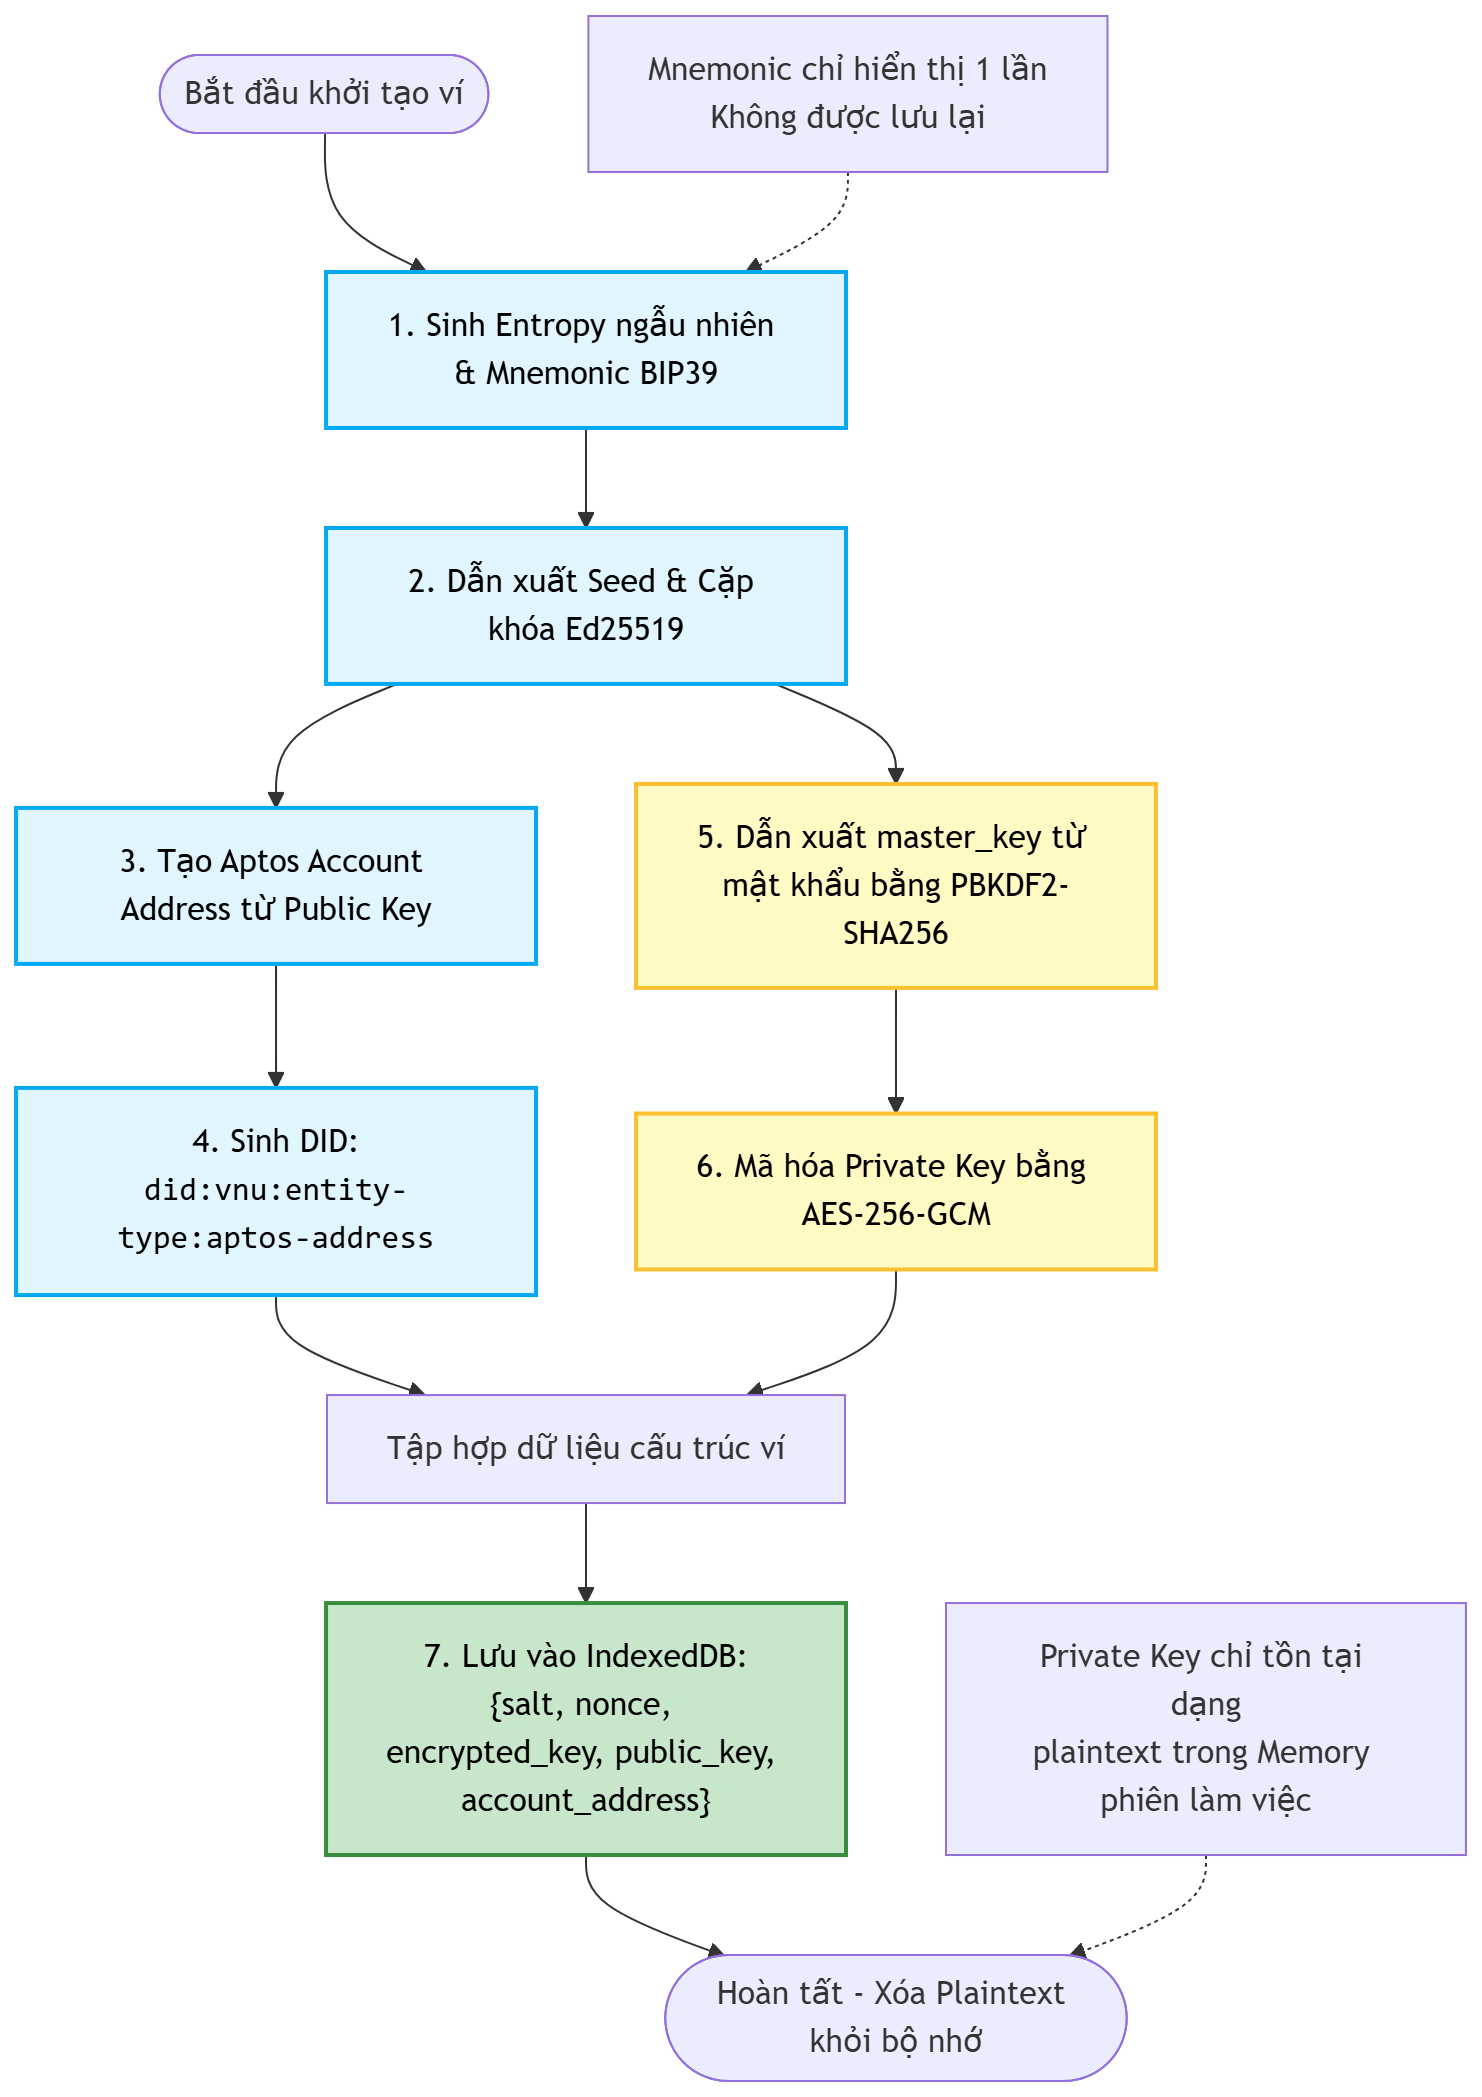
\includegraphics[width=0.5\textwidth]{images/khoi-tao-vi.png}
    \caption{Chuỗi bước sinh khóa và lưu trữ khi khởi tạo ví}
    \label{fig:khoi-tao-vi}
\end{figure}

Sau khi ví được khởi tạo, các thông tin nhạy cảm nằm ở dạng bản mã trong cơ sở dữ liệu cục bộ. Khi người dùng quay lại để đăng nhập, ký xác thực hoặc dựng bản trình bày, trình tự tương tác giữa các thành phần diễn ra như Hình \ref{fig:mo-khoa-va-su-dung}. Điểm cần chú ý trong sơ đồ: khóa riêng dạng rõ chỉ tồn tại trong bộ nhớ phiên làm việc và được giải phóng khi phiên kết thúc, nên bề mặt tấn công bị thu hẹp về đúng khoảng thời gian ví đang mở.

\begin{figure}[H]
    \centering
    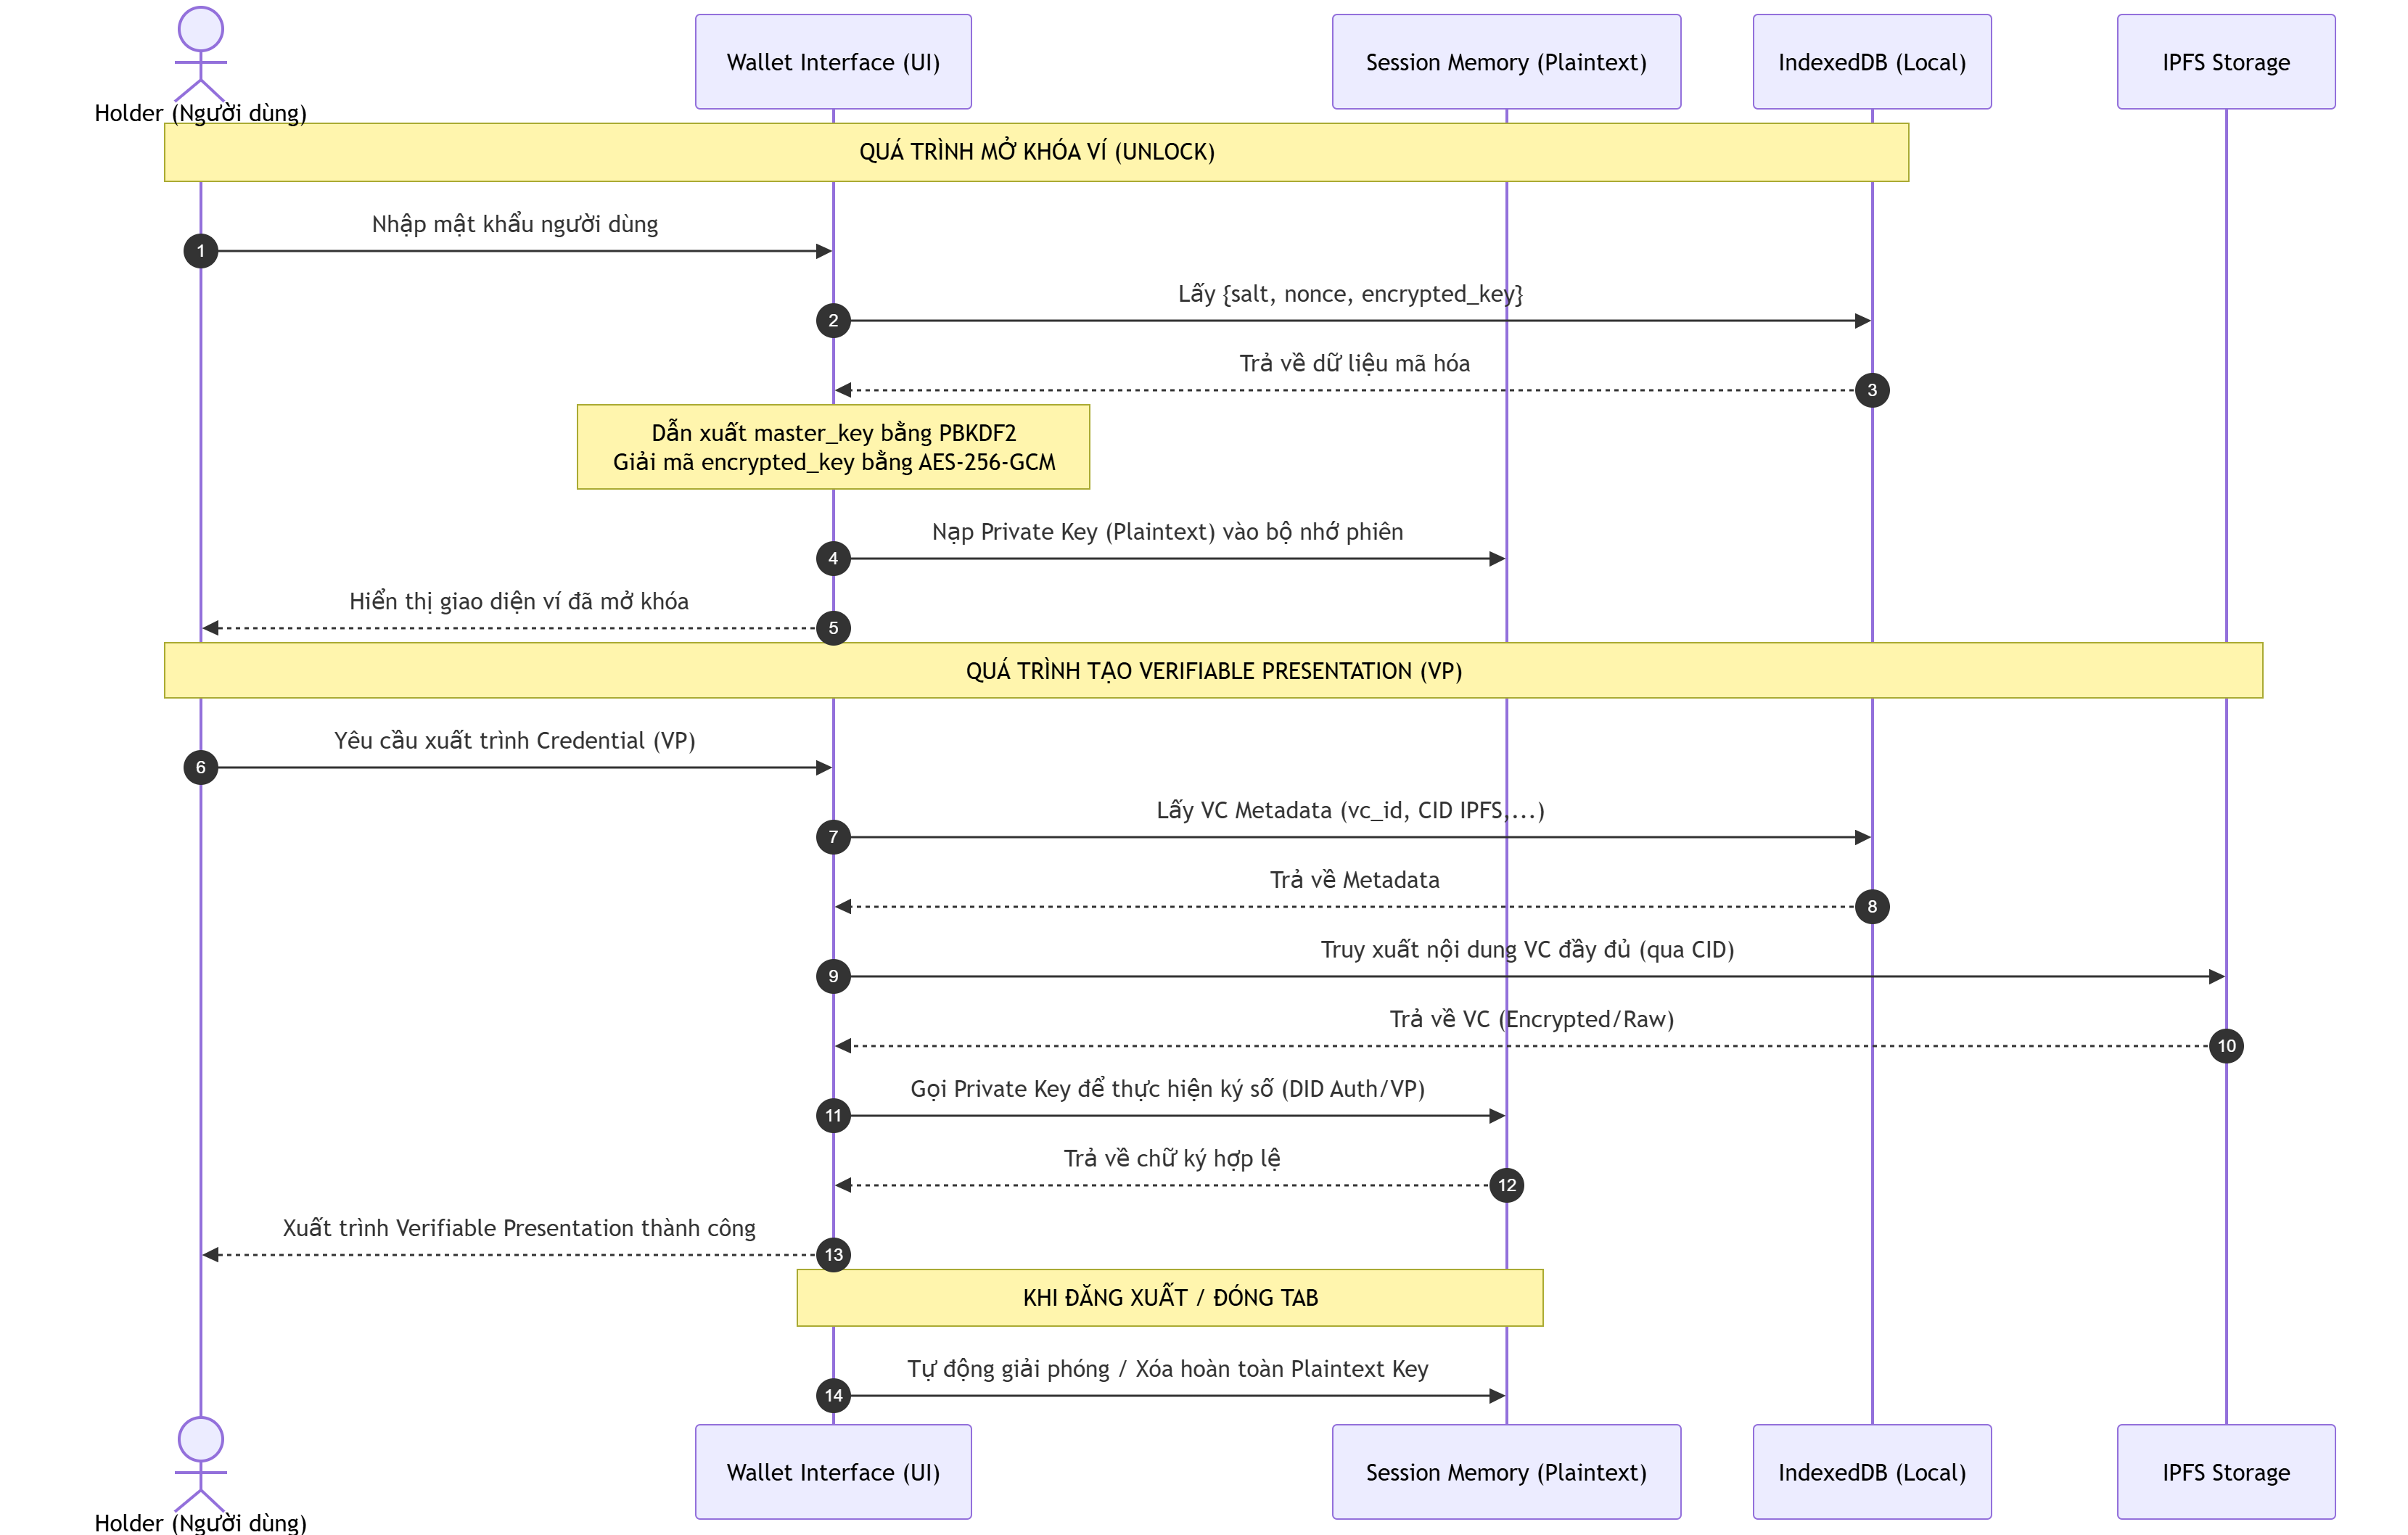
\includegraphics[width=1\textwidth]{images/mo-khoa-su-dung.png}
    \caption{Sơ đồ tuần tự khi mở khóa ví và dựng bản trình bày}
    \label{fig:mo-khoa-va-su-dung}
\end{figure}

Đánh đổi đã chấp nhận và được cảnh báo rõ trên giao diện: \textbf{mất mật khẩu là mất ví}, không có cơ chế đặt lại. Giao diện nhắc người dùng tải bản sao lưu ngay tại thời điểm tạo ví.

Một điểm cần nói rõ về những gì tầng dịch vụ lưu. Dịch vụ chỉ giữ \emph{bản ghi công khai} của mỗi thực thể: địa chỉ, khóa công khai, định danh, vai trò và nhãn hiển thị. Đó là một cuốn danh bạ, không phải một kho tài khoản --- không có giá trị băm mật khẩu, không có khóa riêng, không có cụm từ khôi phục. Hệ quả kiểm chứng được: biết địa chỉ của một người mà không có khóa riêng của họ thì không đăng nhập được.

\subsection{Khôi phục trên thiết bị khác}

Để chủ thể sử dụng được định danh của mình trên thiết bị khác, ví hỗ trợ khôi phục từ cụm từ ghi nhớ. Chuỗi dẫn xuất gồm bốn bước: mười hai từ theo từ điển BIP-39 \cite{BIP39} cho ra một hạt giống; hạt giống đi qua phép dẫn xuất phân cấp theo SLIP-0010 cho họ khóa Ed25519 \cite{SLIP0010} theo một đường dẫn xác định; từ đó suy ra khóa riêng và khóa công khai; và từ khóa công khai suy ra địa chỉ tài khoản.

Đường dẫn dẫn xuất được chọn trùng với đường dẫn mà các ví của hệ sinh thái Move sử dụng, nên một cụm từ ghi nhớ tạo bởi hệ thống này khôi phục được bằng ví phổ thông và ngược lại. Tính tương thích đó đã được kiểm chứng bằng cách đối chiếu kết quả dẫn xuất với bộ công cụ phát triển chính thức của nền tảng trên năm cụm từ ngẫu nhiên, với tiêu chí khớp tuyệt đối ở cả ba giá trị: khóa riêng, khóa công khai và địa chỉ.

Đây là một ví dụ của nguyên tắc kiểm chứng đã nêu ở Mục 1.5.2: giá trị kỳ vọng của phép kiểm không được tự đặt ra mà phải lấy từ một nguồn độc lập. Nếu bộ kiểm chỉ so kết quả dẫn xuất với một hằng số do chính người viết nghĩ ra, nó sẽ đạt kể cả khi phép dẫn xuất sai.

\subsection{Ký và gửi giao dịch không dùng bộ công cụ của nền tảng}

\noindent \textbf{Vấn đề}

Phiên bản đầu của giao diện có một ô {``}Mã giao dịch{''} ở mọi biểu mẫu: người dùng phải mở một ví ngoài, tự gọi hàm hợp đồng, chép mã giao dịch, rồi dán lại vào giao diện. Thiết kế này sai ở hai mức.

Ở mức trải nghiệm, nó đẩy phần khó nhất sang cho người dùng trong khi trình duyệt đã có sẵn khóa riêng trong bộ nhớ tab --- nếu trình duyệt ký được thì nó phải tự ký.

Ở mức dữ liệu, hệ quả nghiêm trọng hơn và không hiển nhiên: vì giao diện không tự gửi giao dịch, nó cũng \emph{không đọc được phản hồi của giao dịch}. Số hiệu của chứng thực do hợp đồng cấp nằm trong sự kiện mà giao dịch phát ra, và vì không đọc được sự kiện đó, trường số hiệu trên chuỗi bị ghi cứng bằng giá trị không --- một trường bịa nằm im trong cơ sở dữ liệu, trông như dữ liệu thật. Lỗi này chỉ lộ ra khi màn hình quản trị cần số hiệu đó để ký thao tác thu hồi.

Nhận định rút ra: thấy một ô {``}dán mã giao dịch{''} trong một giao diện có ví không lưu ký thì đó là dấu hiệu của thiết kế sai, không phải một yêu cầu nghiệp vụ.

\noindent \textbf{Ràng buộc: không thêm bộ công cụ của nền tảng}

Hướng xử lý hiển nhiên là nhúng bộ công cụ phát triển chính thức của nền tảng vào giao diện. Nhưng bộ công cụ đó có kích thước khoảng 4,7\,MB cho một vài phép ký, và việc nhúng nó đưa kích thước gói giao diện lên 4,98\,MB. Với một ứng dụng mà người dùng chủ yếu truy cập qua trình duyệt, đây là một cái giá không tương xứng.

Hướng đã chọn là thực hiện toàn bộ chuỗi thao tác bằng các thư viện mật mã độc lập, nhờ chính nút đầy đủ của mạng thực hiện phép tuần tự hóa nhị phân:

\begin{lstlisting}
POST /v1/transactions/encode_submission   <- giao dich chua ky
   -> chuoi thap luc phan cua thong diep can ky
ed25519.sign(thong diep, khoa rieng trong bo nho)
POST /v1/transactions                     <- giao dich + chu ky
   -> { hash }
GET  /v1/transactions/by_hash/{hash}       lap cho den khi xac nhan
\end{lstlisting}

Kết quả: kích thước gói giao diện giảm từ 4,98\,MB xuống 405\,KB. Đánh đổi là thêm một vòng gọi mạng cho mỗi giao dịch, để nút đầy đủ thực hiện phép tuần tự hóa. Trước khi chọn hướng này, các giá trị do thư viện mật mã độc lập sinh ra --- địa chỉ, khóa công khai và chữ ký --- đã được đối chiếu với bộ công cụ chính thức và cho kết quả khớp tuyệt đối.

\noindent \textbf{Kiểm chứng đường ký trên chuỗi thật}

Một đường ký tự hiện thực cần được kiểm chứng với chuỗi thật, nhưng việc kiểm chứng không nên tạo ra dữ liệu công khai ngoài ý muốn. Hệ thống dùng tuyến mô phỏng giao dịch của nút đầy đủ cho mục đích này. Tuyến này thực thi đầy đủ việc giải mã tham số, tìm hàm, vào thân hàm và tính chi phí, nên chứng minh được rằng cách mã hóa tham số và thứ tự tham số của giao diện là đúng --- mà không ghi bất cứ gì lên chuỗi.

Quá trình kiểm chứng này làm lộ ba chi tiết kỹ thuật không có trong tài liệu và đều từng gây lỗi:

\begin{itemize}
    \item \textbf{Tham số kiểu dãy byte phải được truyền ở dạng chuỗi thập lục phân}, không phải dạng mảng số. Truyền mảng số bị nút đầy đủ từ chối.
    \item \textbf{Nút đầy đủ từ chối mô phỏng một giao dịch có chữ ký hợp lệ.} Để mô phỏng, phải gửi một chữ ký toàn số không kèm khóa công khai \emph{thật} của người gửi.
    \item \textbf{Khóa xác thực trong thông tin tài khoản không phải khóa công khai} --- nó là giá trị băm của khóa công khai. Dùng sai giá trị này làm giao dịch bị từ chối vì khóa xác thực không hợp lệ.
\end{itemize}

\section{Giao diện theo vai trò}

Giao diện được tổ chức theo vai trò, với nguyên tắc: mỗi màn hình chỉ hiển thị những thao tác mà vai trò đó thực sự được phép thực hiện trên chuỗi. Điều này không thay thế việc kiểm quyền --- rào chắn thật vẫn ở hợp đồng --- nhưng tránh để người dùng thực hiện một thao tác chắc chắn thất bại.

Năm quy tắc phân quyền trên giao diện được lấy trực tiếp từ Bảng \ref{tab:role-permission}:

\begin{itemize}
    \item Ô chọn cấp bit ủy quyền bị khóa nếu người đang dùng không phải quản trị viên gốc.
    \item Các thao tác cấp và thu hồi quyền quản trị viên, đề cử người nhận quyền gốc chỉ xuất hiện ở màn hình quản trị gốc, và màn hình đó tự kiểm tra trên chuỗi rằng người đang dùng đúng là quản trị viên gốc.
    \item Thẻ ký nhận quyền gốc nằm ở trang cá nhân, không nằm trong khu quản trị --- vì tại thời điểm ký nhận, người đó vẫn chưa phải quản trị viên gốc.
    \item Nút kích hoạt lại chứng thực chỉ có ở màn hình quản trị viên, không có ở màn hình bên phát hành.
    \item Vai trò hiển thị trong ví được đồng bộ theo dịch vụ mỗi lần đăng nhập, nên một ví khai là chủ thể mà đã được cấp quyền quản trị viên sẽ thấy ngay các màn hình tương ứng.
\end{itemize}

Hai thành phần giao diện đáng được nêu vì chúng giải quyết các vấn đề vận hành thực tế.

\textbf{Thành phần tiến trình giao dịch} hiển thị năm bước của một thao tác ghi --- chuẩn bị dữ liệu, bảo đảm có chi phí giao dịch, ký, chờ chuỗi xác nhận, ghi chỉ mục --- mỗi bước một nhãn riêng. Mã giao dịch xuất hiện như \emph{kết quả} của thao tác kèm liên kết tới trình xem giao dịch, chứ không phải như dữ liệu người dùng phải nhập. Việc tách năm bước có giá trị chẩn đoán: khi thao tác thất bại, người dùng biết nó thất bại ở đâu, và ba nguyên nhân phổ biến nhất --- không đủ chi phí giao dịch, bị hợp đồng từ chối vì thiếu quyền, và chuỗi xác nhận chậm --- có ba cách xử lý khác nhau.

\textbf{Thẻ chi phí giao dịch} hiển thị số dư và một nút xin chi phí thử nghiệm cho chính tài khoản đang dùng. Thẻ này hiện cho mọi vai trò, kể cả chủ thể --- một lựa chọn cần giải thích, vì thoạt nhìn chủ thể không cần đến nó. Lý do: thao tác đăng ký định danh cũng tốn chi phí giao dịch, nên một chủ thể tự đăng ký định danh của mình vẫn cần. Cần nói rõ phạm vi của thành phần này: hệ thống \emph{không có} chức năng chuyển token --- không màn hình, không tuyến dịch vụ, không giao dịch chuyển token nào kể cả để thử nghiệm. Thao tác duy nhất liên quan tới token là việc xin chi phí giao dịch cho chính mình.

Khi chạy ở chế độ không phụ thuộc chuỗi, giao diện \emph{không} gửi giao dịch lên chuỗi, vì gói trên chuỗi có thể chưa tồn tại hoặc không khớp mã nguồn. Ví vẫn ký đúng nội dung giao dịch bằng khóa riêng thật, và tham chiếu gửi lên dịch vụ là giá trị băm của bản đã ký. Giao diện gọi đúng tên của giá trị này là \emph{tham chiếu cục bộ}, không gọi là mã giao dịch, và không đưa liên kết tới trình xem giao dịch. Đây là hệ quả của nguyên tắc ở Mục 4.4.4: một cờ chế độ phải được áp dụng nhất quán ở cả hai phía, và nguồn dữ liệu không được khai sai.

\section{Các kịch bản sử dụng}

Bảy kịch bản dưới đây bao phủ toàn bộ vòng đời văn bằng cùng các luồng quản trị, và được dùng làm căn cứ cho phần đánh giá ở Mục 4.8.

\subsection{Kịch bản 1: Đăng ký định danh}

\begin{figure}[H]
    \centering
    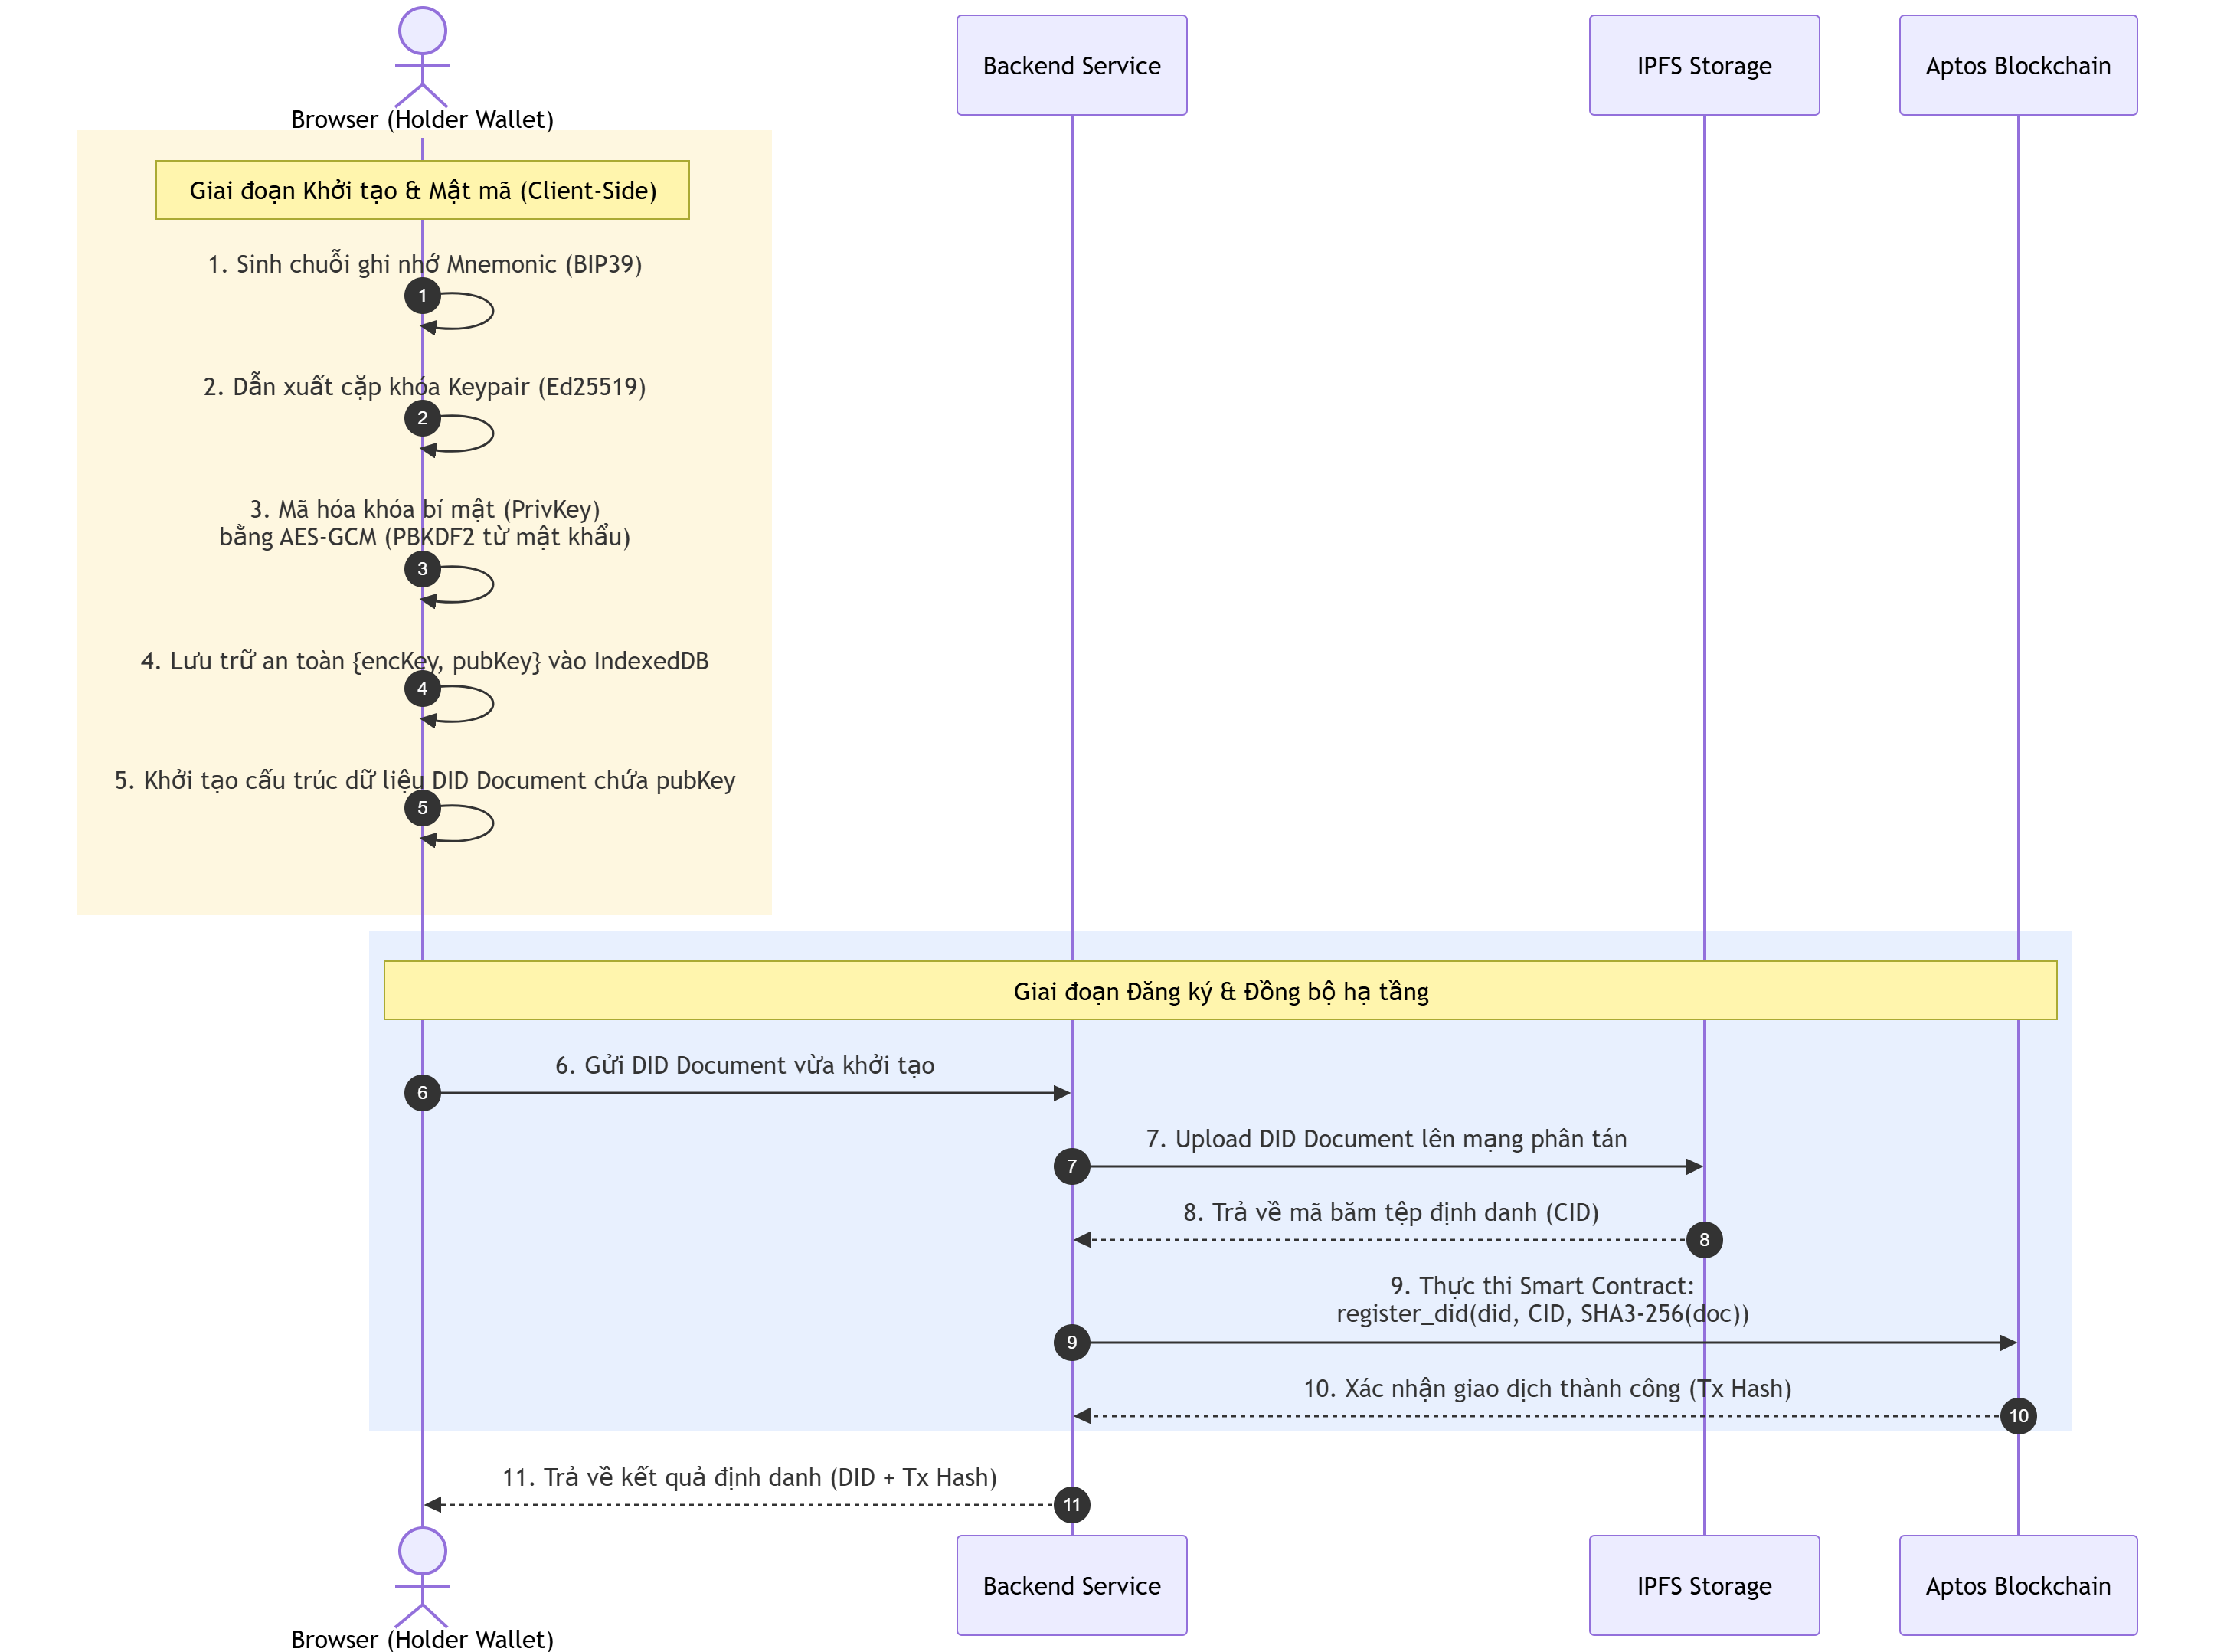
\includegraphics[width=1\textwidth]{images/seq_dang_ky_did_client.png}
    \caption{Sơ đồ tuần tự quy trình đăng ký định danh phía máy khách}
    \label{fig:seq_dang_ky_did_client}
\end{figure}

\begin{longtable}{|p{3.4cm}|p{10.3cm}|}
\caption{Đặc tả kịch bản đăng ký định danh}
\label{tab:did-registration-scenario} \\

\hline
\textbf{Mục} & \textbf{Nội dung} \\
\hline
\endfirsthead

\hline
\textbf{Mục} & \textbf{Nội dung} \\
\hline
\endhead

\hline
\endfoot

\hline
\endlastfoot

Mã kịch bản & KB1 \\
\hline

Tác nhân chính & Mọi vai trò: chủ thể, bên phát hành, quản trị viên, bên xác minh \\
\hline

Thành phần tham gia &
Ví định danh, tầng chuỗi phía máy khách, lớp lưu trữ ngoài chuỗi, mô-đun \cbox{did\_registry}, tầng chỉ mục \\
\hline

Mục đích &
Tạo một định danh phi tập trung và đăng ký siêu dữ liệu của nó lên chuỗi, để bất kỳ bên nào cũng phân giải được \\
\hline

Điều kiện tiên quyết &
\begin{itemize}[leftmargin=*, nosep]
    \item Ví đã được khởi tạo và đang ở trạng thái mở
    \item Địa chỉ của người dùng có đủ chi phí giao dịch
    \item Địa chỉ chưa có định danh đang hoạt động, hoặc định danh cũ đã bị thu hồi
\end{itemize} \\
\hline

Luồng thực hiện chính &
\begin{enumerate}[leftmargin=*, nosep]
    \item Ví dựng chuỗi định danh theo khuôn \cbox{did:vnu:<vai-tro>:<dia-chi>} từ địa chỉ của chính nó
    \item Ví dựng DID Document chứa khóa công khai, hai phương thức xác thực và khẳng định
    \item Giao diện tính giá trị băm SHA3-256 của tài liệu trên bản tuần tự hóa tất định
    \item Tài liệu được ghim lên lớp lưu trữ ngoài chuỗi, nhận về định danh nội dung
    \item Tầng chuỗi dựng giao dịch gọi \cbox{register\_did}, nhờ nút đầy đủ tuần tự hóa, ký bằng khóa riêng trong bộ nhớ, rồi gửi
    \item Giao diện chờ giao dịch được xác nhận và lấy mã giao dịch
    \item Tầng chỉ mục xác minh bốn điều của giao dịch rồi ghi bản ghi vào chỉ mục
\end{enumerate} \\
\hline

Luồng ngoại lệ &
\begin{itemize}[leftmargin=*, nosep]
    \item Ghim lên lớp lưu trữ thất bại $\rightarrow$ dừng ở bước chuẩn bị, không có giao dịch nào được gửi
    \item Không đủ chi phí giao dịch $\rightarrow$ giao diện gợi ý xin chi phí thử nghiệm rồi thử lại
    \item Chuỗi định danh đã tồn tại $\rightarrow$ hợp đồng từ chối với mã lỗi định danh đã được đăng ký
    \item Địa chỉ đã có định danh đang hoạt động $\rightarrow$ hợp đồng từ chối; phải thu hồi định danh cũ trước
    \item Giao dịch thất bại trên chuỗi $\rightarrow$ không có bản ghi nào được ghi vào chỉ mục
\end{itemize} \\
\hline

Kết quả sau cùng &
\begin{itemize}[leftmargin=*, nosep]
    \item Định danh được đăng ký với phiên bản 1 và trạng thái đang hoạt động
    \item Phân giải định danh thành công, giá trị băm tính lại khớp giá trị đã neo
\end{itemize} \\
\hline

Tính chất được kiểm chứng &
F1, F7, N5 --- khóa riêng không rời khỏi trình duyệt trong toàn bộ luồng \\
\hline

\end{longtable}


\subsection{Kịch bản 2: Phê duyệt bên phát hành}

\begin{longtable}{|p{3.4cm}|p{10.3cm}|}
\caption{Đặc tả kịch bản phê duyệt bên phát hành}
\label{tab:onboarding-issuer-scenario} \\

\hline
\textbf{Mục} & \textbf{Nội dung} \\
\hline
\endfirsthead

\hline
\textbf{Mục} & \textbf{Nội dung} \\
\hline
\endhead

\hline
\endfoot

\hline
\endlastfoot

Mã kịch bản & KB2 \\
\hline

Tác nhân chính & Quản trị viên gốc hoặc quản trị viên \\
\hline

Thành phần tham gia &
Ví của người quản trị, mô-đun \cbox{authority}, mô-đun \cbox{did\_registry}, lớp lưu trữ ngoài chuỗi, tầng chỉ mục \\
\hline

Mục đích &
Ghi một bản ghi thẩm quyền lên chuỗi, xác lập rằng một đơn vị được phép cấp một tập loại văn bằng xác định trong một thời hạn xác định \\
\hline

Điều kiện tiên quyết &
\begin{itemize}[leftmargin=*, nosep]
    \item Người thực hiện là quản trị viên gốc hoặc quản trị viên đang hoạt động trên chuỗi
    \item Đơn vị được phê duyệt đã có định danh đang hoạt động
    \item Đơn vị đó chưa giữ vai trò quản trị viên đang hoạt động
\end{itemize} \\
\hline

Luồng thực hiện chính &
\begin{enumerate}[leftmargin=*, nosep]
    \item Người quản trị chọn đơn vị và đánh dấu tập loại văn bằng được phép; giao diện gộp thành mặt nạ bit
    \item Ô chọn bit ủy quyền bị khóa nếu người thực hiện không phải quản trị viên gốc
    \item Người quản trị đặt thời hạn ủy quyền, hoặc để trống nếu vô thời hạn
    \item Nếu có quan hệ ủy quyền, chứng thực ủy quyền được ký và ghim lên lớp lưu trữ ngoài chuỗi
    \item Ví ký giao dịch gọi \cbox{approve\_issuer} với mặt nạ, thời hạn và tham chiếu chứng thực ủy quyền
    \item Hợp đồng kiểm các điều kiện, ghi bản ghi mới với phiên bản tăng thêm một, rồi phát sự kiện
    \item Tầng chỉ mục xác minh giao dịch, cập nhật vai trò trong chỉ mục và ghi nhật ký kiểm toán
\end{enumerate} \\
\hline

Luồng ngoại lệ &
\begin{itemize}[leftmargin=*, nosep]
    \item Người thực hiện không có quyền $\rightarrow$ hợp đồng từ chối với mã lỗi không phải quản trị viên
    \item Quản trị viên cố cấp bit ủy quyền $\rightarrow$ từ chối, chỉ quản trị viên gốc được cấp bit này
    \item Đơn vị chưa có định danh đang hoạt động $\rightarrow$ từ chối với mã lỗi định danh không hoạt động
    \item Đơn vị đang là quản trị viên $\rightarrow$ từ chối với mã lỗi xung đột vai trò
    \item Đơn vị đã là bên phát hành đang hoạt động $\rightarrow$ từ chối; phải thu hồi trước khi cấp lại
    \item Có quan hệ ủy quyền nhưng giá trị băm chứng thực ủy quyền sai độ dài $\rightarrow$ từ chối
\end{itemize} \\
\hline

Luồng thay thế: ủy quyền lại &
Một bên phát hành có bit ủy quyền thực hiện cùng thao tác cho đơn vị cấp dưới, với ba ràng buộc bổ sung do hợp đồng thi hành: phạm vi là tập con của phạm vi mình đang có, thời hạn không vượt thời hạn của mình, và bit ủy quyền không được truyền tiếp \\
\hline

Kết quả sau cùng &
\begin{itemize}[leftmargin=*, nosep]
    \item Bản ghi thẩm quyền tồn tại trên chuỗi và tra cứu được công khai
    \item Bản ghi cũ nếu có vẫn nằm trong tập bản ghi làm dấu vết kiểm toán
    \item Thao tác có mã giao dịch và có một dòng trong nhật ký kiểm toán
\end{itemize} \\
\hline

Tính chất được kiểm chứng &
F3, F4, F5, F12, N1, N2, N3 --- và các hành vi T1, T2 trong mô hình đe dọa \\
\hline

\end{longtable}


\subsection{Kịch bản 3: Cấp phát chứng thực}

\begin{figure}[H]
    \centering
    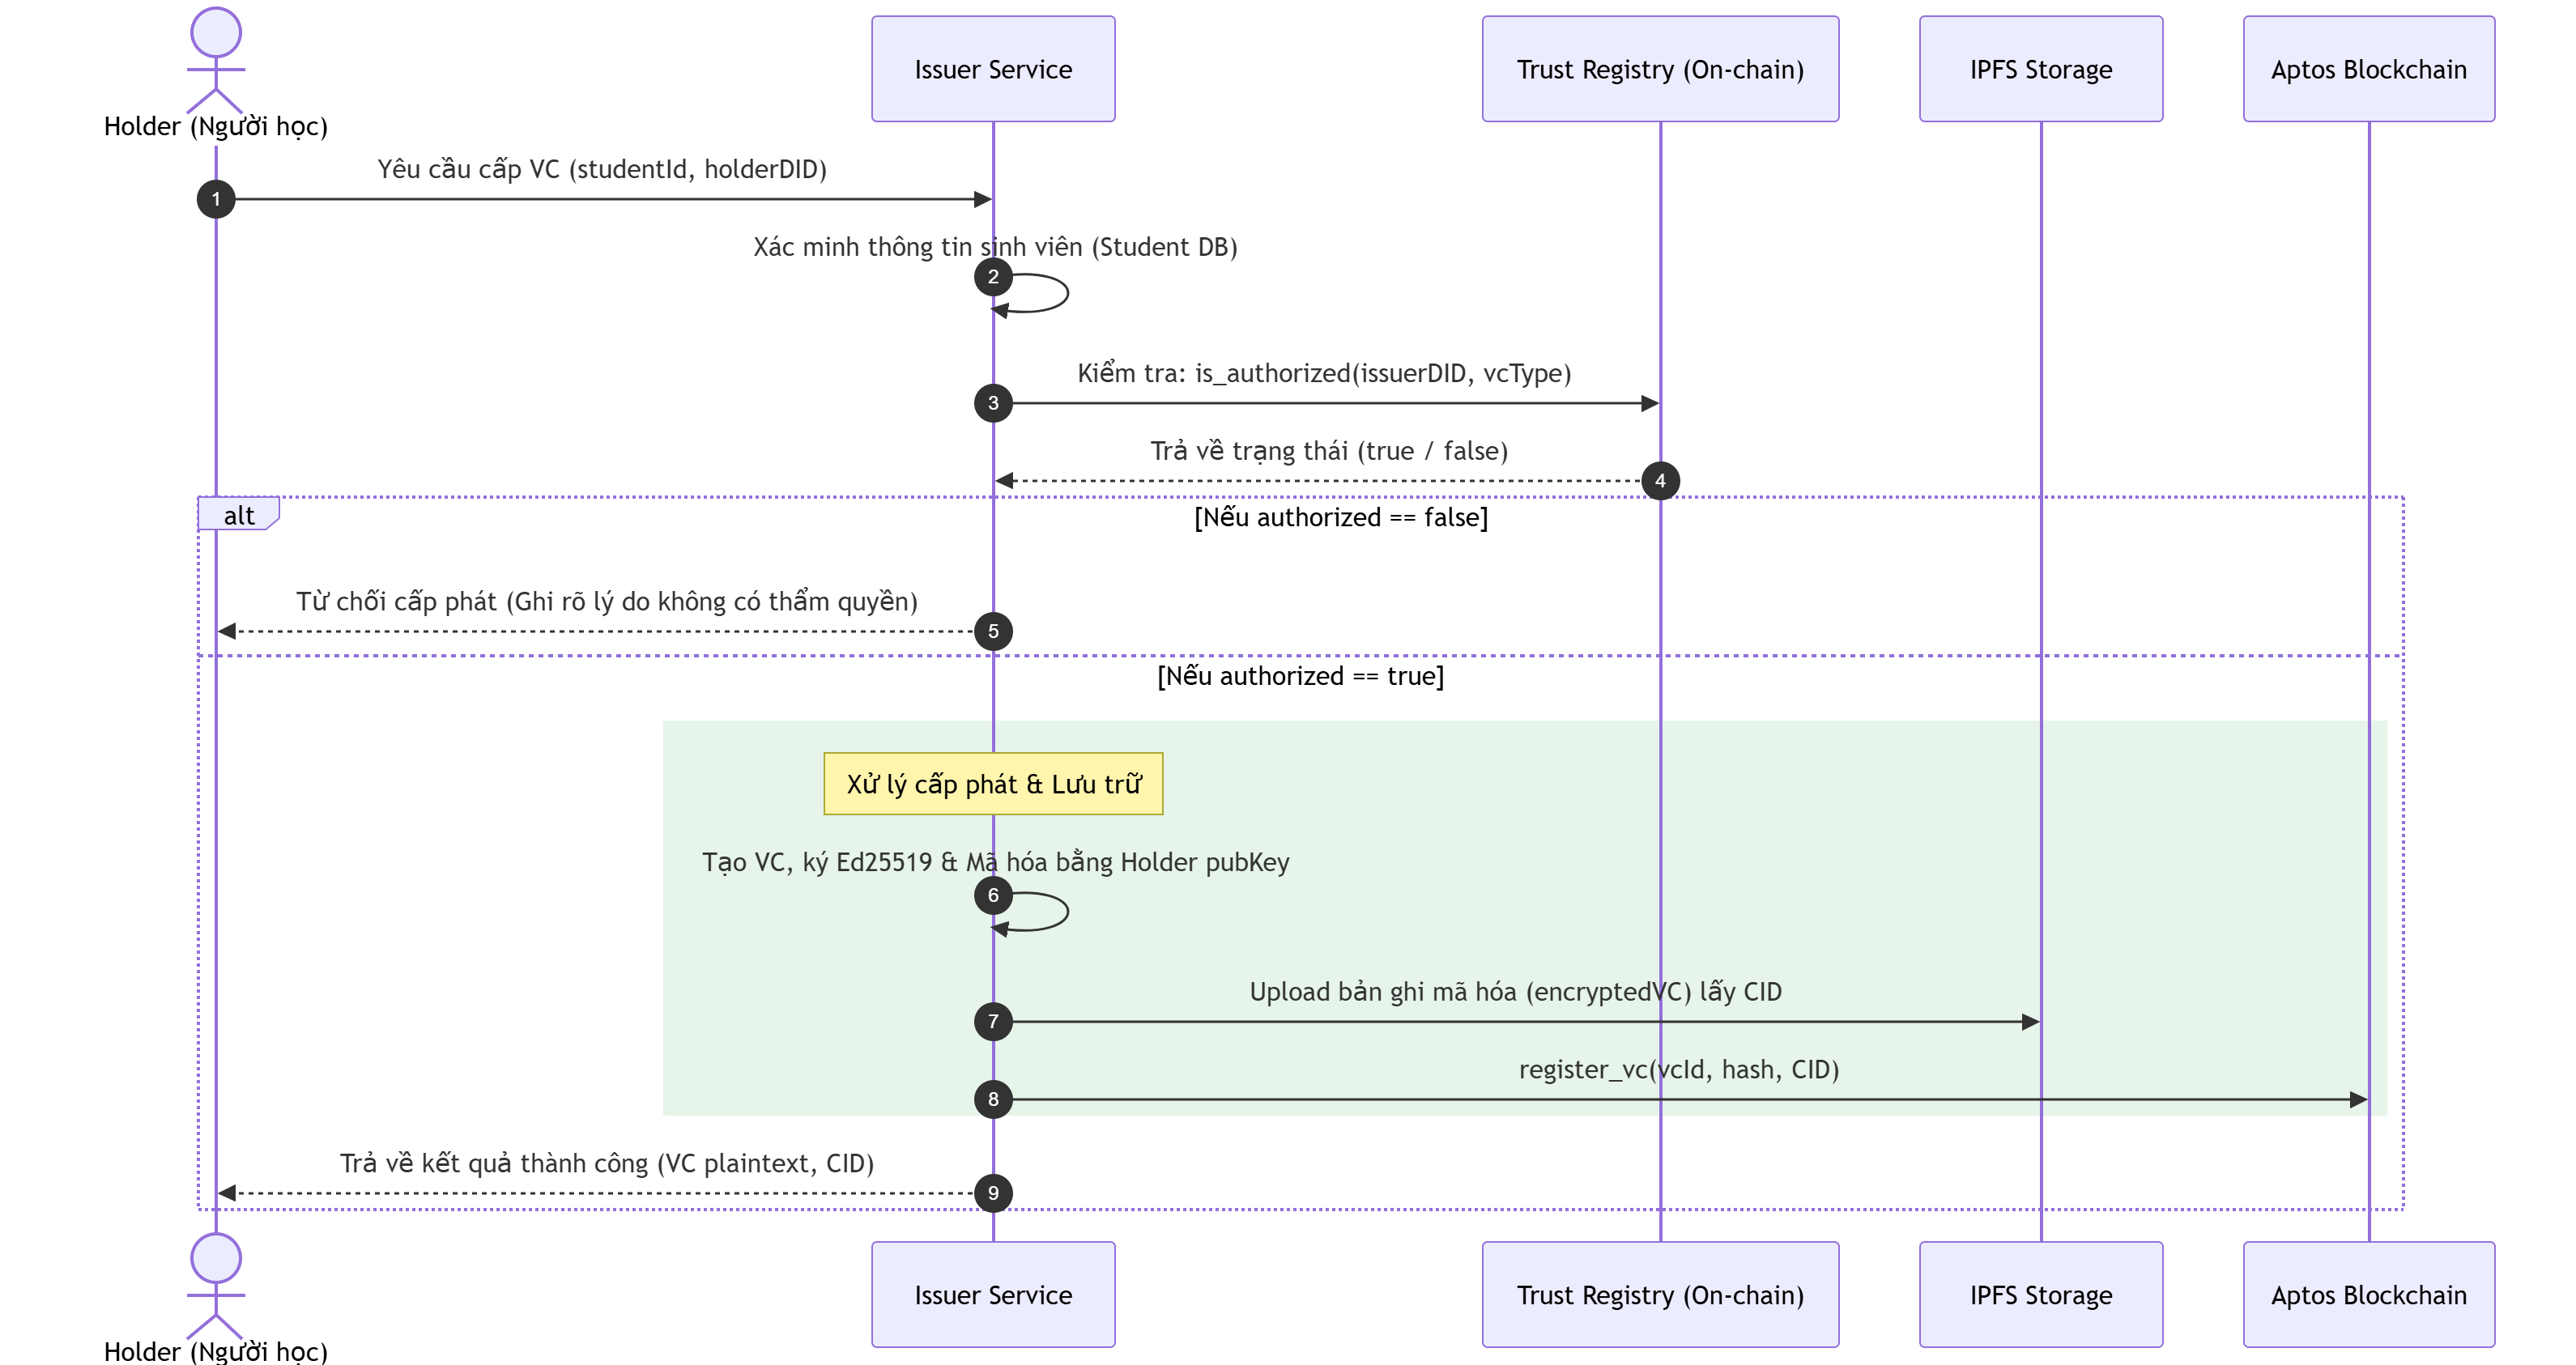
\includegraphics[width=1\textwidth]{images/seq_cap_phat_vc_authorized.png}
    \caption{Sơ đồ tuần tự quy trình cấp phát chứng thực}
    \label{fig:seq_cap_phat_vc_authorized}
\end{figure}

\begin{longtable}{|p{3.4cm}|p{10.3cm}|}
\caption{Đặc tả kịch bản cấp phát chứng thực}
\label{tab:vc-issuance-scenario} \\

\hline
\textbf{Mục} & \textbf{Nội dung} \\
\hline
\endfirsthead

\hline
\textbf{Mục} & \textbf{Nội dung} \\
\hline
\endhead

\hline
\endfoot

\hline
\endlastfoot

Mã kịch bản & KB3 \\
\hline

Tác nhân chính & Bên phát hành \\
\hline

Thành phần tham gia &
Ví của bên phát hành, lớp lưu trữ ngoài chuỗi, mô-đun \cbox{vc\_registry}, mô-đun \cbox{authority}, tầng chỉ mục \\
\hline

Mục đích &
Tạo một chứng thực văn bằng, ký bằng khóa riêng của bên phát hành, và neo giá trị băm của nó lên chuỗi \\
\hline

Điều kiện tiên quyết &
\begin{itemize}[leftmargin=*, nosep]
    \item Bên phát hành có bản ghi thẩm quyền đang hoạt động và chưa hết hạn
    \item Loại văn bằng cần cấp nằm trong phạm vi được phép
    \item Cả bên phát hành và chủ thể đều có định danh đang hoạt động
\end{itemize} \\
\hline

Luồng thực hiện chính &
\begin{enumerate}[leftmargin=*, nosep]
    \item Bên phát hành nhập dữ liệu văn bằng và định danh của chủ thể
    \item Giao diện dựng chứng thực theo mô hình dữ liệu W3C, với các thuộc tính riêng trong không gian tên của hệ thống
    \item Tính giá trị băm của nội dung chứng thực và giá trị băm của định danh chứng thực
    \item Ví ký nội dung chứng thực trên bản tuần tự hóa tất định
    \item Nội dung được ghim lên lớp lưu trữ ngoài chuỗi, nhận về định danh nội dung
    \item Ví ký giao dịch gọi \cbox{issue\_vc} với bảy tham số, trong đó có thời hạn
    \item Hợp đồng kiểm thẩm quyền, kiểm trạng thái định danh hai bên, kiểm độ dài các giá trị băm và định dạng định danh nội dung, rồi ghi bản ghi
    \item Giao diện đọc số hiệu chứng thực từ sự kiện trong phản hồi giao dịch
    \item Tầng chỉ mục xác minh giao dịch rồi ghi bản ghi kèm số hiệu thật
\end{enumerate} \\
\hline

Luồng ngoại lệ &
\begin{itemize}[leftmargin=*, nosep]
    \item Bên phát hành không có thẩm quyền $\rightarrow$ hợp đồng từ chối với mã lỗi bên phát hành không hoạt động
    \item Loại văn bằng ngoài phạm vi $\rightarrow$ từ chối với mã lỗi loại văn bằng không được phép
    \item Thẩm quyền đã hết hạn $\rightarrow$ từ chối với mã lỗi thẩm quyền đã hết hạn
    \item Định danh của chủ thể không hoạt động $\rightarrow$ từ chối
    \item Thời hạn chứng thực đặt vào quá khứ $\rightarrow$ từ chối, vì cấp một chứng thực đã hết hạn là vô nghĩa
    \item Giá trị băm của định danh chứng thực đã tồn tại $\rightarrow$ từ chối, chống cấp trùng
\end{itemize} \\
\hline

Kết quả sau cùng &
\begin{itemize}[leftmargin=*, nosep]
    \item Bản ghi chứng thực tồn tại trên chuỗi với trạng thái đang hoạt động
    \item Số hiệu chứng thực trong chỉ mục là số hiệu thật do hợp đồng cấp, đọc từ sự kiện
    \item Bộ đếm tổng đã cấp và bộ đếm số đang hiệu lực đều tăng
\end{itemize} \\
\hline

Tính chất được kiểm chứng &
F6, F12, N3, N4 --- và các hành vi T1, T2, T3, T9 trong mô hình đe dọa \\
\hline

\end{longtable}


\subsection{Kịch bản 4: Trình bày và xác minh}

\begin{longtable}{|p{3.4cm}|p{10.3cm}|}
\caption{Đặc tả kịch bản trình bày và xác minh}
\label{tab:vp-verification-scenario} \\

\hline
\textbf{Mục} & \textbf{Nội dung} \\
\hline
\endfirsthead

\hline
\textbf{Mục} & \textbf{Nội dung} \\
\hline
\endhead

\hline
\endfoot

\hline
\endlastfoot

Mã kịch bản & KB4 \\
\hline

Tác nhân chính & Chủ thể (trình bày) và bên xác minh (kiểm tra) \\
\hline

Thành phần tham gia &
Ví của chủ thể, lớp lưu trữ ngoài chuỗi, ba mô-đun hợp đồng, dịch vụ xác minh \\
\hline

Mục đích &
Chủ thể chứng minh mình sở hữu một tập văn bằng hợp lệ; bên xác minh kiểm chứng điều đó độc lập với bên phát hành \\
\hline

Điều kiện tiên quyết &
\begin{itemize}[leftmargin=*, nosep]
    \item Chủ thể có ít nhất một chứng thực trong ví
    \item Ví đang ở trạng thái mở
\end{itemize} \\
\hline

Luồng thực hiện chính &
\begin{enumerate}[leftmargin=*, nosep]
    \item Chủ thể chọn tập chứng thực muốn trình bày
    \item Giao diện dựng bản trình bày và ví ký bằng khóa riêng của chủ thể
    \item Bản trình bày được ghim lên lớp lưu trữ ngoài chuỗi
    \item Hệ thống sinh một liên kết chia sẻ có thời hạn, có thể thu hồi, kèm mã QR
    \item Bên xác minh mở liên kết và yêu cầu chạy quy trình xác minh
    \item Dịch vụ xác minh thực hiện bảy bước và trả báo cáo theo từng bước
    \item Bên xác minh có thể lưu kết quả vào lịch sử xác minh của mình
\end{enumerate} \\
\hline

Bảy bước kiểm tra &
\begin{enumerate}[leftmargin=*, nosep]
    \item Truy xuất bản trình bày từ lớp lưu trữ ngoài chuỗi
    \item Đối chiếu giá trị băm của bản trình bày
    \item Kiểm chữ ký của người trình bày bằng khóa công khai của chủ thể
    \item Kiểm trạng thái định danh của người trình bày
    \item Kiểm trạng thái hiệu lực của từng chứng thực, gồm cả thời điểm hết hạn
    \item Đối chiếu nội dung từng chứng thực với giá trị băm đã neo trên chuỗi
    \item Kiểm trạng thái thẩm quyền của bên phát hành từng chứng thực
\end{enumerate} \\
\hline

Luồng ngoại lệ &
\begin{itemize}[leftmargin=*, nosep]
    \item Liên kết chia sẻ đã hết hạn hoặc đã bị chủ thể thu hồi $\rightarrow$ dịch vụ từ chối truy cập
    \item Không tải được bản trình bày $\rightarrow$ bước một thất bại, và báo cáo phân biệt rõ đây là lỗi khả dụng chứ không phải lỗi hợp lệ
    \item Một hoặc nhiều bước thất bại $\rightarrow$ xem kịch bản KB7
\end{itemize} \\
\hline

Kết quả sau cùng &
\begin{itemize}[leftmargin=*, nosep]
    \item Báo cáo xác minh gồm trạng thái và chi tiết của cả bảy bước
    \item Kết quả tổng thể hợp lệ khi và chỉ khi cả bảy bước đạt
    \item Toàn bộ quy trình hoàn tất mà không cần liên hệ bên phát hành
\end{itemize} \\
\hline

Tính chất được kiểm chứng &
F8, F9, F10, N7, N8, N11 --- và các hành vi T7, T8, T15 trong mô hình đe dọa \\
\hline

\end{longtable}


\subsection{Kịch bản 5: Thu hồi thẩm quyền của bên phát hành}

\begin{longtable}{|p{3.4cm}|p{10.3cm}|}
\caption{Đặc tả kịch bản thu hồi thẩm quyền của bên phát hành}
\label{tab:issuer-revocation-scenario} \\

\hline
\textbf{Mục} & \textbf{Nội dung} \\
\hline
\endfirsthead

\hline
\textbf{Mục} & \textbf{Nội dung} \\
\hline
\endhead

\hline
\endfoot

\hline
\endlastfoot

Mã kịch bản & KB5 \\
\hline

Tác nhân chính & Quản trị viên gốc hoặc quản trị viên \\
\hline

Thành phần tham gia &
Ví của người quản trị, mô-đun \cbox{authority}, tầng chỉ mục, dịch vụ xác minh \\
\hline

Mục đích &
Đình chỉ hoặc thu hồi thẩm quyền cấp phát của một đơn vị, sao cho các lần xác minh sau đó phát hiện được trạng thái này \\
\hline

Điều kiện tiên quyết &
Người thực hiện là quản trị viên gốc hoặc quản trị viên đang hoạt động; đơn vị bị xử lý có bản ghi thẩm quyền \\
\hline

Phân biệt ba thao tác &
\begin{itemize}[leftmargin=*, nosep]
    \item \textbf{Đình chỉ}: trạng thái chuyển sang tạm đình chỉ. Quyền vẫn còn trong bản ghi, chỉ bị khóa. Vai trò trong chỉ mục \textbf{không đổi}
    \item \textbf{Kích hoạt lại}: đưa trạng thái từ tạm đình chỉ trở về đang hoạt động
    \item \textbf{Thu hồi}: trạng thái chuyển sang đã thu hồi. Vai trò trong chỉ mục hạ xuống chủ thể, nhưng đơn vị vẫn giữ định danh và các văn bằng của riêng mình
\end{itemize} \\
\hline

Luồng thực hiện chính &
\begin{enumerate}[leftmargin=*, nosep]
    \item Người quản trị chọn đơn vị, chọn thao tác và nhập lý do
    \item Ví ký giao dịch gọi hàm tương ứng trên mô-đun \cbox{authority}
    \item Hợp đồng cập nhật trạng thái, ghi lý do và dấu thời gian, rồi phát sự kiện
    \item Tầng chỉ mục xác minh giao dịch, cập nhật vai trò nếu cần và ghi nhật ký kiểm toán
    \item Từ thời điểm này, bước thứ bảy của quy trình xác minh phát hiện trạng thái mới
\end{enumerate} \\
\hline

Hệ quả đối với các chứng thực đã cấp &
\begin{itemize}[leftmargin=*, nosep]
    \item Các chứng thực do đơn vị đó cấp \textbf{vẫn hợp lệ về mặt kỹ thuật}: chữ ký vẫn đúng, nội dung vẫn khớp giá trị băm đã neo
    \item Nhưng chúng \textbf{bị từ chối ở bước kiểm thẩm quyền}, và báo cáo xác minh nêu rõ nguyên nhân là thẩm quyền của bên phát hành chứ không phải lỗi nội dung
    \item Đơn vị \textbf{vẫn thu hồi được} các chứng thực mình đã cấp, theo nguyên tắc bất đối xứng ở Mục 3.4.5
\end{itemize} \\
\hline

Luồng ngoại lệ &
\begin{itemize}[leftmargin=*, nosep]
    \item Người thực hiện không có quyền $\rightarrow$ hợp đồng từ chối
    \item Kích hoạt lại một đơn vị không ở trạng thái tạm đình chỉ $\rightarrow$ từ chối với mã lỗi tương ứng
    \item Thu hồi một đơn vị đã bị thu hồi $\rightarrow$ từ chối, tránh ghi hai bản ghi cho cùng một thao tác
\end{itemize} \\
\hline

Kết quả sau cùng &
Trạng thái mới tra cứu được công khai trên chuỗi; bản ghi cũ giữ nguyên làm dấu vết; thao tác có mã giao dịch và một dòng nhật ký \\
\hline

Tính chất được kiểm chứng &
F3, F10, F12, N1, N2 --- và nguyên tắc bất đối xứng ở Mục 3.4.5 \\
\hline

\end{longtable}


\subsection{Kịch bản 6: Thu hồi chứng thực}

\begin{longtable}{|p{3.4cm}|p{10.3cm}|}
\caption{Đặc tả kịch bản thu hồi chứng thực}
\label{tab:vc-revocation-scenario} \\

\hline
\textbf{Mục} & \textbf{Nội dung} \\
\hline
\endfirsthead

\hline
\textbf{Mục} & \textbf{Nội dung} \\
\hline
\endhead

\hline
\endfoot

\hline
\endlastfoot

Mã kịch bản & KB6 \\
\hline

Tác nhân chính & Bên phát hành (thu hồi, đình chỉ) hoặc quản trị viên (thu hồi, kích hoạt lại) \\
\hline

Thành phần tham gia &
Ví của người thực hiện, mô-đun \cbox{vc\_registry}, tầng chỉ mục, dịch vụ xác minh \\
\hline

Mục đích &
Cập nhật trạng thái của một chứng thực để các lần xác minh sau đó từ chối nó, dù chữ ký vẫn hợp lệ về mặt toán học \\
\hline

Điều kiện tiên quyết &
\begin{itemize}[leftmargin=*, nosep]
    \item Chứng thực tồn tại trên chuỗi
    \item Với thao tác của bên phát hành: người thực hiện đúng là bên đã cấp chứng thực đó, và định danh của họ còn hoạt động. \textbf{Không} yêu cầu thẩm quyền còn hiệu lực
    \item Với thao tác của quản trị viên: người thực hiện là quản trị viên gốc hoặc quản trị viên đang hoạt động
\end{itemize} \\
\hline

Phân biệt bốn thao tác &
\begin{itemize}[leftmargin=*, nosep]
    \item \textbf{Đình chỉ} (bên phát hành): trạng thái tạm thời, có thể đảo ngược --- nhưng chỉ quản trị viên đảo ngược được
    \item \textbf{Kích hoạt lại} (chỉ quản trị viên): đưa chứng thực từ tạm đình chỉ về đang hoạt động
    \item \textbf{Thu hồi} (bên phát hành): tuyên bố vĩnh viễn, không thể đảo ngược
    \item \textbf{Thu hồi} (quản trị viên): dùng khi cần cưỡng chế, chẳng hạn khi bên phát hành không còn hoạt động
\end{itemize} \\
\hline

Luồng thực hiện chính &
\begin{enumerate}[leftmargin=*, nosep]
    \item Người thực hiện chọn chứng thực trong bảng danh sách và chọn thao tác
    \item Giao diện đọc số hiệu chứng thực trên chuỗi từ chỉ mục --- số này không do người dùng gõ tay, để tránh gõ nhầm một chữ số và xử lý nhầm văn bằng của người khác
    \item Ví ký giao dịch gọi hàm tương ứng kèm lý do
    \item Hợp đồng kiểm điều kiện, cập nhật trạng thái, giảm bộ đếm số đang hiệu lực, rồi phát sự kiện
    \item Tầng chỉ mục xác minh giao dịch, cập nhật trạng thái trong chỉ mục và ghi nhật ký
\end{enumerate} \\
\hline

Hai trường hợp đặc biệt được hỗ trợ &
\begin{itemize}[leftmargin=*, nosep]
    \item \textbf{Đơn vị đã hết hạn ủy quyền vẫn thu hồi được} chứng thực mình đã cấp. Đây là kịch bản quan trọng nhất của nguyên tắc bất đối xứng: phát hiện gian lận thường xảy ra sau khi chu kỳ ủy quyền đã kết thúc
    \item \textbf{Chứng thực đã hết hạn vẫn thu hồi được}, vì hết hạn và thu hồi mang hai thông điệp khác nhau: hết hạn nói chứng thực không còn giá trị từ một thời điểm, thu hồi nói nó chưa bao giờ đáng tin
\end{itemize} \\
\hline

Luồng ngoại lệ &
\begin{itemize}[leftmargin=*, nosep]
    \item Người thực hiện không phải bên đã cấp $\rightarrow$ từ chối với mã lỗi không phải bên cấp
    \item Bên phát hành cố kích hoạt lại chứng thực $\rightarrow$ từ chối, thao tác này chỉ thuộc quản trị viên
    \item Thu hồi một chứng thực đã bị thu hồi $\rightarrow$ từ chối
    \item Định danh của bên thực hiện đã bị thu hồi $\rightarrow$ từ chối
\end{itemize} \\
\hline

Kết quả sau cùng &
Trạng thái mới tra cứu được trên chuỗi; bước thứ năm của quy trình xác minh từ chối chứng thực từ thời điểm này; bộ đếm số đang hiệu lực giảm \\
\hline

Tính chất được kiểm chứng &
F11, F12, N2 --- và các hành vi T13 trong mô hình đe dọa \\
\hline

\end{longtable}


\subsection{Kịch bản 7: Xác minh thất bại}

\begin{longtable}{|p{3.4cm}|p{10.3cm}|}
\caption{Đặc tả kịch bản xác minh thất bại}
\label{tab:verification-failure-scenario} \\

\hline
\textbf{Mục} & \textbf{Nội dung} \\
\hline
\endfirsthead

\hline
\textbf{Mục} & \textbf{Nội dung} \\
\hline
\endhead

\hline
\endfoot

\hline
\endlastfoot

Mã kịch bản & KB7 \\
\hline

Tác nhân chính & Bên xác minh \\
\hline

Mục đích &
Kiểm chứng rằng quy trình xác minh không chỉ từ chối đúng các trường hợp không hợp lệ, mà còn \textbf{nêu đúng nguyên nhân} --- điều kiện cần để bên xác minh biết phải xử lý thế nào \\
\hline

Nguyên tắc thiết kế được kiểm chứng &
Quy trình không dừng ở bước thất bại đầu tiên mà chạy hết cả bảy bước, rồi trả báo cáo đầy đủ. Lý do: một bản trình bày có thể hỏng ở nhiều chỗ, và bên xác minh cần thấy toàn bộ vấn đề \\
\hline

Trường hợp A: nội dung chứng thực bị sửa sau khi cấp &
Bước 6 (đối chiếu nội dung với giá trị băm đã neo) \textbf{thất bại}, trong khi bước 5 (trạng thái hiệu lực) và bước 7 (thẩm quyền bên phát hành) \textbf{vẫn đạt}. Đây là trường hợp quan trọng nhất của kịch bản: nó chứng minh một quy trình thiếu bước 6 sẽ chấp nhận chứng thực đã bị sửa. Tương ứng hành vi T7 \\
\hline

Trường hợp B: bản trình bày do thực thể khác ký &
Bước 3 (chữ ký của người trình bày) thất bại. Các bước còn lại có thể vẫn đạt, vì bản thân chứng thực không bị sửa gì. Tương ứng hành vi T8 \\
\hline

Trường hợp C: chứng thực đã bị thu hồi &
Bước 5 thất bại, nêu rõ trạng thái là đã thu hồi kèm lý do. Bước 6 vẫn đạt, vì nội dung không bị sửa --- đây là điểm phân biệt với trường hợp A \\
\hline

Trường hợp D: chứng thực đã hết hạn &
Bước 5 thất bại với trạng thái đã hết hạn. Báo cáo phân biệt rõ hết hạn với thu hồi, vì hai trạng thái này mang hai thông điệp khác nhau \\
\hline

Trường hợp E: bên phát hành đã bị thu hồi thẩm quyền &
Bước 7 thất bại. Các bước kỹ thuật đều đạt, vì chứng thực vẫn nguyên vẹn và chữ ký vẫn đúng. Tương ứng kịch bản KB5 \\
\hline

Trường hợp F: định danh của người trình bày đã bị thu hồi &
Bước 4 thất bại, nêu rõ trạng thái định danh. Trường hợp này tương ứng tình huống chủ thể đã thu hồi định danh cũ sau khi lộ khóa riêng \\
\hline

Trường hợp G: DID Document bị thay đổi trên lớp lưu trữ &
Phép đối chiếu giá trị băm trong quy trình phân giải định danh thất bại, nên bước 4 không hoàn tất. Tương ứng hành vi T15 \\
\hline

Trường hợp H: không tải được bản trình bày &
Bước 1 thất bại. Báo cáo phân biệt rõ đây là \textbf{lỗi khả dụng} chứ không phải \textbf{lỗi hợp lệ} --- một bản trình bày không tải được không có nghĩa là văn bằng không hợp lệ \\
\hline

Trường hợp I: liên kết chia sẻ hết hạn hoặc đã bị thu hồi &
Dịch vụ từ chối ngay ở bước mở liên kết, với mã trạng thái riêng phân biệt với lỗi không tìm thấy \\
\hline

Kết quả sau cùng &
\begin{itemize}[leftmargin=*, nosep]
    \item Mọi trường hợp đều bị từ chối ở kết quả tổng thể
    \item Báo cáo nêu đúng bước nào thất bại và vì nguyên nhân gì
    \item Ba nhóm nguyên nhân --- nội dung bị sửa, trạng thái không còn hiệu lực, thẩm quyền không còn --- được phân biệt rõ, theo Bảng \ref{tab:verification-matrix}
\end{itemize} \\
\hline

Tính chất được kiểm chứng &
F9, F10, N6 --- và các hành vi T7, T8, T15 trong mô hình đe dọa \\
\hline

\end{longtable}


\section{Chiến lược kiểm thử và kết quả kiểm chứng}

\subsection{Cấu trúc bộ kiểm thử}

Hệ thống được kiểm chứng bằng chín bộ kiểm thử ở các tầng khác nhau, mỗi bộ nhằm chứng minh một loại tính chất.

\begin{longtable}{|p{3.3cm}|c|p{8.4cm}|}
\caption{Chín bộ kiểm thử và tính chất mà mỗi bộ nhằm chứng minh}
\label{tab:test-suites} \\

\hline
\textbf{Bộ kiểm thử} & \textbf{Số phép} & \textbf{Tính chất được chứng minh} \\
\hline
\endfirsthead

\hline
\textbf{Bộ kiểm thử} & \textbf{Số phép} & \textbf{Tính chất được chứng minh} \\
\hline
\endhead

\hline
\endfoot

\hline
\endlastfoot

Kiểm thử đơn vị hợp đồng
& 126
& Logic phân quyền đúng đắn. Trong đó 83 phép dựng một thao tác vi phạm và khẳng định nó bị từ chối với đúng mã lỗi dự kiến
\\ \hline

Đối chiếu tên hàm hợp đồng
& 19
& Tên hàm khớp nhau giữa ba nơi gọi: mã Move, hai cài đặt tầng chỉ mục, và tầng chuỗi của giao diện
\\ \hline

Kiểm thử đầu cuối
& 19 $\times$ 2
& Các luồng chính hoạt động đầu cuối. Cùng một bộ chạy lên cả hai cài đặt qua biến môi trường chỉ địa chỉ dịch vụ
\\ \hline

Kiểm thử luồng nghiệp vụ
& 31 $\times$ 2
& Toàn bộ vòng đời văn bằng và các luồng quản trị, bao gồm nội dung thực của nhật ký kiểm toán
\\ \hline

Đối chiếu hai cài đặt
& 59
& Hai cài đặt trả cùng kết quả và cùng mã trạng thái cho cùng một yêu cầu, kể cả với dữ liệu vào không hợp lệ
\\ \hline

Phát hiện nội dung bị sửa
& 7 $\times$ 2
& Bước đối chiếu nội dung với giá trị băm đã neo phát hiện được nội dung bị sửa sau khi cấp, trong khi bước kiểm trạng thái vẫn đạt
\\ \hline

Kiểm thử chế độ nghiêm ngặt
& 6
& Ở chế độ phụ thuộc chuỗi, hệ thống vẫn chặn mã giao dịch bịa đặt và vẫn từ chối bên tự khai là bên phát hành
\\ \hline

Kiểm thử ví
& 17
& Khóa riêng không rời khỏi trình duyệt: kiểm toàn bộ gói tin gửi lên dịch vụ, không gói nào chứa khóa riêng hay mật khẩu
\\ \hline

Kiểm thử khôi phục thiết bị khác
& 17
& Khôi phục bằng cụm từ ghi nhớ cho đúng cặp khóa và địa chỉ; biết địa chỉ mà không có khóa thì đăng nhập thất bại
\\ \hline

Đối chiếu tầng chuỗi với nút đầy đủ
& 12
& Cách mã hóa tham số và thứ tự tham số của giao diện đúng với hợp đồng trên chuỗi thật, kiểm bằng tuyến mô phỏng nên không ghi gì lên chuỗi
\\ \hline

Phép đo tải
& 905.160 yêu cầu
& Hệ thống không sinh lỗi chức năng dưới tải; đồng thời lượng hoá chính độ tin cậy của phép đo (Mục 4.9)
\\ \hline

\end{longtable}


Ba đặc điểm của chiến lược này cần được nêu.

Thứ nhất, \textbf{phần lớn các phép kiểm trên hợp đồng là phép kiểm trường hợp vi phạm}. Trong 126 phép kiểm, có 83 phép --- tức khoảng 66\% --- dựng một thao tác vi phạm và khẳng định rằng nó bị từ chối với đúng mã lỗi dự kiến. Tỷ lệ này là có chủ đích, theo nhận định ở Mục 1.5.2: một quy tắc phân quyền chỉ được coi là hoạt động khi có một phép kiểm chứng minh nó thực sự chặn được điều nó tuyên bố chặn.

Thứ hai, \textbf{cùng một bộ kiểm thử đầu cuối được chạy lên cả hai cài đặt của tầng chỉ mục} thông qua một biến môi trường chỉ định địa chỉ dịch vụ. Đây là cách bảo đảm hai cài đặt thực sự tương đương, thay vì mỗi bên có một bộ kiểm riêng viết theo chính hành vi của nó.

Thứ ba, \textbf{bộ điều khiển kiểm thử cũng cần được kiểm thử}. Tập lệnh chạy toàn bộ bộ kiểm thử ban đầu dẫn đầu ra của mỗi bộ qua một lệnh lọc để in vài dòng cuối. Vì mã thoát của một đường ống trong vỏ lệnh là mã thoát của lệnh cuối cùng, và lệnh lọc luôn thành công, tập lệnh in {``}tất cả đạt{''} \emph{bất kể} có bộ nào thất bại. Lỗi này bị phát hiện khi một bộ báo 52 trên 53 phép đạt mà dòng tổng kết vẫn xanh. Sau khi sửa, cách kiểm chứng tập lệnh là cho một bộ thất bại có chủ ý và xác nhận rằng nó bị bắt.

\subsection{Kết quả kiểm chứng chức năng}

\begin{longtable}{|p{5.4cm}|p{3.1cm}|p{5.2cm}|}
\caption{Kết quả kiểm chứng chức năng ở lần chạy gần nhất}
\label{tab:test-results} \\

\hline
\textbf{Thành phần hoặc bộ kiểm} & \textbf{Kết quả} & \textbf{Ghi chú} \\
\hline
\endfirsthead

\hline
\textbf{Thành phần hoặc bộ kiểm} & \textbf{Kết quả} & \textbf{Ghi chú} \\
\hline
\endhead

\hline
\endfoot

\hline
\endlastfoot

Hợp đồng thông minh (Move)
& \textbf{126 / 126 đạt}
& Bao gồm 83 phép kiểm trường hợp vi phạm; mười vấn đề rà soát đều có phép kiểm chứng minh đã sửa \\
\hline

Đối chiếu tên hàm ba nơi gọi
& \textbf{19 / 19 khớp}
& Tăng từ 16 phép khi bổ sung tầng chuỗi của giao diện làm nơi gọi thứ ba \\
\hline

Tầng chỉ mục, cài đặt TypeScript
& 0 lỗi kiểm kiểu; \textbf{19 / 19} đầu cuối; \textbf{31 / 31} luồng nghiệp vụ
& Biên dịch ở chế độ kiểm kiểu nghiêm ngặt \\
\hline

Tầng chỉ mục, cài đặt Go
& Biên dịch và kiểm tĩnh sạch; \textbf{19 / 19} đầu cuối; \textbf{31 / 31} luồng nghiệp vụ
& Chạy cùng bộ kiểm thử với cài đặt TypeScript \\
\hline

Đối chiếu hai cài đặt
& \textbf{59 / 59 khớp}
& Tăng từ 53 phép sau khi bổ sung các tuyến còn thiếu ở cài đặt Go \\
\hline

Giao diện
& 0 lỗi kiểm kiểu; gói phát hành 405\,KB
& Giảm từ 4,98\,MB sau khi loại bộ công cụ của nền tảng \\
\hline

Kiểm thử ví
& \textbf{17 / 17 đạt}
& Gồm phép kiểm rằng không gói tin nào gửi lên dịch vụ chứa khóa riêng hoặc mật khẩu \\
\hline

Khôi phục trên thiết bị khác
& \textbf{17 / 17 đạt}
& Gồm phép kiểm rằng biết địa chỉ mà không có khóa thì đăng nhập bị từ chối \\
\hline

Phát hiện nội dung bị sửa
& \textbf{7 / 7 đạt} $\times$ 2 cài đặt
& Xem phân tích tại Mục 4.8.3 \\
\hline

Chế độ nghiêm ngặt
& \textbf{6 / 6 đạt}
& Chạy ở chế độ phụ thuộc chuỗi \\
\hline

Tầng chuỗi với nút đầy đủ
& \textbf{11 / 12 đạt}
& Phép còn lại thất bại vì gói trên chuỗi là bản xuất bản trước đợt sửa; xem phân tích tại Mục 4.8.2 \\
\hline

Phép đo tải, bốn thí nghiệm
& \textbf{0 lỗi / 905.160 yêu cầu}
& 0 phản hồi vượt hạn mức. Kết luận về ngưỡng độ trễ: xem Mục 4.9.6 \\
\hline

\end{longtable}


Hai kết quả cần được giải thích.

\textbf{Bộ đối chiếu tầng chuỗi với nút đầy đủ đạt 11 trên 12 phép.} Phép còn lại là phép đối chiếu tập hàm trong giao diện chương trình của gói \emph{đang nằm trên chuỗi} với tập hàm trong mã nguồn hiện tại. Phép này thất bại vì gói trên chuỗi là bản được xuất bản trước đợt sửa mười vấn đề rà soát: hàm cấp phát chứng thực trên chuỗi còn nhận sáu tham số thay vì bảy --- tức chưa có tham số thời hạn --- và hai hàm của cơ chế chuyển quyền gốc hai bước chưa tồn tại, trong khi hàm chuyển quyền một bước thì vẫn còn. Nói cách khác, phép kiểm này đang báo đúng một trạng thái thật và sẽ còn thất bại cho tới khi gói được xuất bản lại. Hệ quả đối với kết luận của chương: các kết quả về logic phân quyền ở Mục 4.8.3 được kiểm chứng trên bộ kiểm thử của hợp đồng --- tức trên mã nguồn đã sửa --- chứ không trên gói đang nằm trên chuỗi.

\textbf{Bộ đối chiếu tên hàm hợp đồng tăng từ 16 lên 19 phép} khi tầng chuỗi của giao diện được thêm vào làm nơi gọi thứ ba. Việc mở rộng này phát hiện ngay một sai lệch thật, đã nêu ở Mục 4.4.3. Nhận định rút ra: thêm một nơi gọi tên hàm hợp đồng thì phải mở rộng bộ bắt lệch ngay tại thời điểm đó, không phải khi nào nhớ ra.

\subsection{Kiểm chứng khả năng phát hiện gian lận}

Phần này đánh giá yêu cầu N6: mỗi kịch bản trong mô hình đe dọa ở Mục 3.7.2 phải bị chặn, và thông điệp từ chối phải khớp đúng nguyên nhân thật.

\begin{longtable}{|c|p{3.9cm}|p{3.4cm}|p{4.5cm}|}
\caption{Kết quả kiểm chứng khả năng phát hiện các hành vi trong mô hình đe dọa}
\label{tab:detection-results} \\

\hline
\textbf{Mã} & \textbf{Hành vi} & \textbf{Nơi bị chặn} & \textbf{Bộ kiểm chứng minh} \\
\hline
\endfirsthead

\hline
\textbf{Mã} & \textbf{Hành vi} & \textbf{Nơi bị chặn} & \textbf{Bộ kiểm chứng minh} \\
\hline
\endhead

\hline
\endfoot

\hline
\endlastfoot

T1 & Tự khai là bên phát hành rồi cấp văn bằng
& Hợp đồng, phép kiểm thẩm quyền
& Kiểm thử đơn vị hợp đồng; kiểm thử chế độ nghiêm ngặt
\\ \hline

T2 & Cấp loại văn bằng ngoài phạm vi
& Hợp đồng, phép giao bit
& Kiểm thử đơn vị hợp đồng
\\ \hline

T3 & Cấp văn bằng sau khi thẩm quyền hết hạn
& Hợp đồng, đối chiếu thời hạn
& Kiểm thử đơn vị hợp đồng
\\ \hline

T4 & Khai báo mã giao dịch không tồn tại
& Tầng dịch vụ, phép kiểm tồn tại
& Kiểm thử chế độ nghiêm ngặt
\\ \hline

T5 & Tái sử dụng giao dịch thật thuộc loại thao tác khác
& Tầng dịch vụ, so khớp tên hàm
& Kiểm thử chế độ nghiêm ngặt; đối chiếu tên hàm
\\ \hline

T6 & Tái sử dụng giao dịch của người khác
& Tầng dịch vụ, so khớp người gửi
& Kiểm thử chế độ nghiêm ngặt
\\ \hline

T7 & Sửa nội dung văn bằng sau khi cấp
& Quy trình xác minh, bước thứ sáu
& Bộ kiểm phát hiện nội dung bị sửa, cả hai cài đặt
\\ \hline

T8 & Trình bày chứng thực của người khác
& Quy trình xác minh, bước thứ ba
& Kiểm thử luồng nghiệp vụ
\\ \hline

T9 & Khai báo giá trị băm sai
& Tầng dịch vụ, tính lại giá trị băm
& Kiểm thử đầu cuối; đối chiếu hai cài đặt
\\ \hline

T10 & Gửi lại chữ ký đăng nhập đã thu được
& Tầng dịch vụ, số dùng một lần
& Kiểm thử ví; khôi phục thiết bị khác
\\ \hline

T11 & Lợi dụng vai trò trong phiên để vượt quyền
& Tầng dịch vụ và hợp đồng
& Kiểm thử chế độ nghiêm ngặt
\\ \hline

T12 & Gán quyền gốc cho địa chỉ không ai kiểm soát
& Hợp đồng, cơ chế hai bước
& Kiểm thử đơn vị hợp đồng
\\ \hline

T13 & Tự đình chỉ rồi tự kích hoạt lại chứng thực
& Hợp đồng, phân tách thẩm quyền
& Kiểm thử đơn vị hợp đồng; kiểm thử luồng nghiệp vụ
\\ \hline

T14 & Đăng ký chuỗi định danh đã thuộc thực thể khác
& Hợp đồng, phép kiểm duy nhất
& Kiểm thử đơn vị hợp đồng
\\ \hline

T15 & Cổng truy cập trả về nội dung khác nội dung đã đăng ký
& Quy trình phân giải, bước đối chiếu giá trị băm
& Bộ kiểm phát hiện nội dung bị sửa
\\ \hline

\end{longtable}


Hai bộ kiểm trong bảng trên được xây dựng riêng cho mục đích này và đáng được mô tả chi tiết hơn.

\textbf{Bộ kiểm phát hiện nội dung bị sửa} nhằm chứng minh rằng bước thứ sáu của quy trình xác minh không dư thừa. Bộ kiểm thực hiện ba việc: cấp một chứng thực và xác minh nó để xác nhận toàn bộ bảy bước đều đạt; sửa một trường trong nội dung chứng thực \emph{trực tiếp trong chỉ mục}, mô phỏng đúng kịch bản T7; rồi xác minh lại và khẳng định hai điều --- bước đối chiếu nội dung với giá trị băm đã neo \emph{thất bại}, và bước kiểm trạng thái hiệu lực \emph{vẫn đạt}. Khẳng định thứ hai là phần quan trọng: nó chứng minh rằng một quy trình xác minh chỉ theo dõi trạng thái sẽ bỏ sót đúng loại tấn công này, nên bước thứ sáu là cần thiết chứ không phải một phép kiểm thừa.

Quá trình xây dựng bộ kiểm này cũng làm lộ một vấn đề thuộc loại đã nêu ở Mục 4.4.5. Hàm đối chiếu nội dung với giá trị băm trên chuỗi đã tồn tại trong mã nguồn từ đầu, với một tên gọi nghe như đang bảo vệ tính toàn vẹn, nhưng \emph{không tuyến nào gọi tới nó} --- và ở cài đặt Go thì hàm đó không có. Người đọc mã sẽ tưởng nội dung chứng thực đang được đối chiếu với chuỗi, trong khi thực tế không. Một hàm được khai báo mà không ai gọi là một cái bẫy, vì nó tạo cảm giác an toàn mà không cung cấp sự an toàn.

\textbf{Bộ kiểm chế độ nghiêm ngặt} chứng minh rằng ở chế độ phụ thuộc chuỗi, hệ thống vẫn chặn mã giao dịch bịa đặt và vẫn từ chối bên tự khai là bên phát hành. Bộ kiểm này cần thiết vì phần lớn các bộ kiểm thử tự động khác chạy ở chế độ không phụ thuộc chuỗi để không cần mạng; nếu không có bộ kiểm riêng cho chế độ nghiêm ngặt, không có gì bảo đảm rằng các rào chắn ở chế độ đó còn hoạt động.

Trong quá trình xây dựng các bộ kiểm này, ba lớp lỗi phương pháp đã được xử lý và đáng ghi lại:

\begin{itemize}
    \item \textbf{Phép kiểm đạt chưa chắc vì lý do đúng.} Phép kiểm {``}mã giao dịch bịa đặt bị từ chối{''} ban đầu cho kết quả đạt, nhưng nguyên nhân thật là một định danh nội dung sai định dạng bị chặn trước, nên bước xác minh giao dịch chưa từng được thực thi. Mọi phép kiểm trường hợp vi phạm phải đọc thông điệp lỗi để xác nhận đúng nguyên nhân.
    \item \textbf{Dữ liệu giả phải đúng hình dạng dữ liệu thật.} Định danh nội dung giả phải tuân đúng khuôn dạng của định danh nội dung thật, nếu không nó bị chính bộ kiểm tra định dạng chặn trước khi chạm tới logic cần kiểm.
    \item \textbf{Phép kiểm thất bại vì hạ tầng thì không chứng minh được gì.} Bộ kiểm thử chạy nhiều kịch bản đăng nhập liên tiếp nên dính giới hạn tần suất một cách ngẫu nhiên. Vì không bộ nào khẳng định hành vi của giới hạn tần suất, tập lệnh chạy kiểm thử nâng giới hạn cho cả lượt chạy rồi trả lại --- thay vì rải các lệnh chờ và trông vào may mắn.
\end{itemize}

\section{Đánh giá hiệu năng}

\subsection{Thiết kế phép đo}

Phần đánh giá hiệu năng của bản thảo đầu tiên báo cáo một bảng số liệu thu từ \emph{một} lượt đo cho mỗi tuyến, ở \emph{một} mức đồng thời, với 120 yêu cầu mỗi tuyến. Khi rà soát lại, cách làm đó không trả lời được ba câu hỏi mà một phép đo cần trả lời trước khi con số của nó có nghĩa:

\begin{itemize}
    \item \textbf{Số đo có lặp lại được không?} Nếu chạy lại cùng phép đo cho con số khác hẳn, thì giá trị báo cáo là một mẫu ngẫu nhiên, không phải một đặc tính của hệ thống.
    \item \textbf{Hệ thống hành xử thế nào khi tải tăng?} Một con số ở một mức đồng thời không nói gì về điểm bão hoà.
    \item \textbf{Vì sao báo phân vị 95 mà không báo giá trị trung bình?} Đây là lựa chọn cần được chứng minh bằng dữ liệu, không phải bằng quy ước.
\end{itemize}

Vì vậy phép đo được thiết kế lại thành bốn thí nghiệm, tổng cộng \textbf{905.160 yêu cầu}:

\begin{enumerate}
    \item \textbf{Độ lặp lại} --- lặp cùng một phép đo 15 lượt cho mỗi tuyến và mỗi cài đặt, ở mức 12 yêu cầu đồng thời, để lượng hoá độ phân tán.
    \item \textbf{Ảnh hưởng của số mẫu} --- giữ nguyên mức đồng thời, thay đổi số mẫu mỗi lượt từ 60 đến 4000, mỗi mức lặp 12 lượt, nhằm phân biệt hai giả thuyết: độ trễ bản chất đã dao động, hay số mẫu quá ít.
    \item \textbf{Quét mức đồng thời} --- bảy mức từ 1 đến 64, mỗi điểm lặp 5 lượt với tối thiểu 1000 yêu cầu mỗi lượt, báo trung vị kèm khoảng nhỏ nhất--lớn nhất.
    \item \textbf{Phân bố độ trễ} --- một lượt lớn 1500 yêu cầu mỗi tuyến, giữ lại độ trễ của từng yêu cầu để dựng hàm phân bố tích luỹ.
\end{enumerate}

Toàn bộ dữ liệu thô được lưu dạng JSON, và các biểu đồ dưới đây được sinh tự động từ dữ liệu đó bằng một tập lệnh riêng. Việc tách bước đo khỏi bước vẽ có một lý do cụ thể: số liệu trong biểu đồ nhúng trực tiếp trong mã nguồn báo cáo nên kiểm chứng được từng con số, và vẽ lại không cần đo lại. Bốn thí nghiệm tương ứng với bốn tập lệnh trong mã nguồn --- \cbox{bench-sweep.mjs} cho thí nghiệm 1 và 4, \cbox{bench-samplesize.mjs} cho thí nghiệm 2, \cbox{bench-sweep2.mjs} cho thí nghiệm 3 --- và tập lệnh sinh biểu đồ là \cbox{bench-plot.mjs}.

Về môi trường đo, một đặc điểm quan trọng cần nêu trước vì nó quyết định cách đọc kết quả: bộ sinh tải, hai tiến trình dịch vụ và cơ sở dữ liệu \emph{cùng chạy trên một máy} có khoảng 3,9\,GB bộ nhớ. Bộ sinh tải vì vậy cạnh tranh tài nguyên với chính hệ thống đang được đo.

\subsection{Thí nghiệm 1: phép đo không lặp lại được ở số mẫu nhỏ}

% SINH TỰ ĐỘNG bởi scripts/bench-plot.mjs — đừng sửa tay.
% Nguồn dữ liệu: .bench/repeat.json
% Bảy cột với hai cột "x ± y" thì ở cỡ chữ thường sẽ tràn lề 92pt — thu nhỏ cỡ
% chữ và khoảng đệm cột thay vì cắt bớt cột, vì cột cuối chính là bằng chứng.
\begingroup
\footnotesize
\setlength{\tabcolsep}{4pt}
\begin{longtable}{|c|l|r|r|r|r|r|}
\caption{Độ lặp lại của phép đo: 15 lượt độc lập cho mỗi tuyến và mỗi cài đặt}
\label{tab:bench-repeat} \\

\hline
\textbf{Cài đặt} & \textbf{Tuyến} & \textbf{yc/giây} & \textbf{CV (\%)} & \textbf{p95 (ms)} & \textbf{CV (\%)} & \textbf{p95 min--max} \\
\hline
\endfirsthead

\hline
\textbf{Cài đặt} & \textbf{Tuyến} & \textbf{yc/giây} & \textbf{CV (\%)} & \textbf{p95 (ms)} & \textbf{CV (\%)} & \textbf{p95 min--max} \\
\hline
\endhead

\hline
\endfoot

\hline
\endlastfoot

TS & \texttt{/health} & 1146 $\pm$ 923 & 80.6 & 45.5 $\pm$ 33.1 & 72.7 & 6.8--139.2 \\
GO & \texttt{/health} & 2974 $\pm$ 1274 & 42.8 & 16.3 $\pm$ 19.0 & 116.2 & 4.7--59.3 \\
TS & \texttt{/stats} & 1470 $\pm$ 894 & 60.8 & 41.3 $\pm$ 31.1 & 75.2 & 5.1--105.5 \\
GO & \texttt{/stats} & 4229 $\pm$ 1808 & 42.7 & 13.2 $\pm$ 27.2 & 205.4 & 2.6--107.0 \\
TS & \texttt{/did/resolve} & 1326 $\pm$ 447 & 33.7 & 18.2 $\pm$ 8.2 & 44.9 & 9.0--32.5 \\
GO & \texttt{/did/resolve} & 2443 $\pm$ 874 & 35.8 & 15.3 $\pm$ 20.0 & 130.6 & 4.3--80.3 \\
TS & \texttt{/lookup} & 1525 $\pm$ 666 & 43.7 & 19.3 $\pm$ 14.5 & 75.3 & 5.8--56.9 \\
GO & \texttt{/lookup} & 2663 $\pm$ 1053 & 39.6 & 12.0 $\pm$ 11.2 & 93.0 & 4.5--47.8 \\
TS & \texttt{/auth/me} & 577 $\pm$ 225 & 39.1 & 40.1 $\pm$ 21.1 & 52.5 & 17.6--82.9 \\
GO & \texttt{/auth/me} & 1868 $\pm$ 661 & 35.4 & 16.2 $\pm$ 14.3 & 88.3 & 5.9--56.3 \\
TS & \texttt{/holder/credentials} & 1535 $\pm$ 335 & 21.8 & 16.6 $\pm$ 13.0 & 78.3 & 8.1--59.8 \\
GO & \texttt{/holder/credentials} & 2842 $\pm$ 1102 & 38.8 & 10.5 $\pm$ 9.1 & 86.7 & 4.3--40.3 \\

\end{longtable}
\endgroup


% SINH TỰ ĐỘNG bởi scripts/bench-plot.mjs — đừng sửa tay.
% Nguồn dữ liệu: .bench/repeat.json  (15 lượt mỗi tuyến, đo 2026-10-13T14:30:43.508Z)
\begin{figure}[H]
\centering
\begin{tikzpicture}
\begin{axis}[
    name=plotR,
    width=0.95\textwidth, height=5.4cm,
    ybar, bar width=7pt,
    xlabel={}, ylabel={Độ trễ p95 (ms)},
    xtick={0,1,2,3,4,5}, xticklabels={/health, /stats, /did/resolve, /lookup, /auth/me, /holder/credentials},
    x tick label style={font=\scriptsize, rotate=20, anchor=north east},
    tick label style={font=\footnotesize}, label style={font=\small},
    ymin=0,
    grid=both, grid style={gray!18},
    error bars/y dir=both, error bars/y explicit,
    legend style={font=\scriptsize, at={(0.98,0.98)}, anchor=north east, draw=gray!40},
    title={(a) p95 trung bình qua 15 lượt đo, thanh sai số là một độ lệch chuẩn},
    title style={font=\small},
]
    \addplot[fill=blue!35, draw=blue!60!black, error bars/error bar style={black}] coordinates {(0,45.52) +- (0,33.10) (1,41.32) +- (0,31.09) (2,18.17) +- (0,8.15) (3,19.28) +- (0,14.51) (4,40.12) +- (0,21.07) (5,16.62) +- (0,13.01)};
    \addlegendentry{TypeScript}
    \addplot[fill=orange!45, draw=orange!70!black, error bars/error bar style={black}] coordinates {(0,16.33) +- (0,18.97) (1,13.23) +- (0,27.17) (2,15.33) +- (0,20.01) (3,12.05) +- (0,11.21) (4,16.23) +- (0,14.34) (5,10.52) +- (0,9.12)};
    \addlegendentry{Go}
\end{axis}
\begin{axis}[
    at={(plotR.below south west)}, anchor=above north west, yshift=-0.9cm,
    width=0.95\textwidth, height=4.2cm,
    ybar, bar width=7pt,
    ylabel={Hệ số biến thiên của p95 (\%)},
    xtick={0,1,2,3,4,5}, xticklabels={/health, /stats, /did/resolve, /lookup, /auth/me, /holder/credentials},
    x tick label style={font=\scriptsize, rotate=20, anchor=north east},
    tick label style={font=\footnotesize}, label style={font=\small},
    ymin=0,
    grid=both, grid style={gray!18},
    legend style={font=\scriptsize, at={(0.98,0.98)}, anchor=north east, draw=gray!40},
    title={(b) Hệ số biến thiên --- càng cao thì số đo một lượt càng ít ý nghĩa},
    title style={font=\small},
]
    \addplot[fill=blue!35, draw=blue!60!black] coordinates {(0,72.7) (1,75.2) (2,44.9) (3,75.3) (4,52.5) (5,78.3)};
    \addlegendentry{TypeScript}
    \addplot[fill=orange!45, draw=orange!70!black] coordinates {(0,116.2) (1,205.4) (2,130.6) (3,93.0) (4,88.3) (5,86.7)};
    \addlegendentry{Go}
\end{axis}
\end{tikzpicture}
\caption{Độ lặp lại của phép đo độ trễ: cùng một phép đo (120 yêu cầu, 12 yêu cầu đồng thời) chạy lại 15 lần trên cùng một máy và cùng một cấu hình.}
\label{fig:bench-repeat}
\end{figure}


Kết quả rõ ràng và không thuận lợi cho bản thảo trước. Hệ số biến thiên của phân vị 95 --- tỉ số giữa độ lệch chuẩn và giá trị trung bình --- nằm trong khoảng \textbf{44,9\%} đến \textbf{205,4\%}, trung bình 93,3\%. Nói cách khác, ở mức 120 yêu cầu mỗi lượt, độ lệch chuẩn của p95 xấp xỉ bằng chính giá trị trung bình của nó.

Thông lượng ổn định hơn nhưng không nhiều: hệ số biến thiên 21,8--80,6\%, trung bình 42,9\%.

Hệ quả trực tiếp: \textbf{các giá trị p95 trong bảng số liệu của bản thảo đầu không phải là đặc tính của hệ thống mà là một mẫu ngẫu nhiên}. Chúng đã được loại khỏi báo cáo. Đây là một ví dụ của nguyên tắc đã nêu tại Mục 1.5.2 --- một phép đo không kiểm được độ lặp lại thì không chứng minh được điều gì --- và lần này nguyên tắc đó áp dụng cho chính phần đánh giá của nghiên cứu.

\subsection{Thí nghiệm 2: số mẫu giảm được nhiễu nhưng không loại bỏ được}

Thí nghiệm 1 cho thấy số đo dao động, nhưng chưa cho biết \emph{vì sao}. Có hai giả thuyết dẫn tới hai cách xử lý khác nhau: nếu độ trễ bản chất đã dao động thì phải báo p95 kèm độ lệch chuẩn; nếu 120 mẫu là quá ít thì chỉ cần tăng số mẫu.

% SINH TỰ ĐỘNG bởi scripts/bench-plot.mjs — đừng sửa tay.
% Nguồn dữ liệu: .bench/samplesize.json
\begin{table}[H]
\centering
\caption{Hệ số biến thiên của p95 theo số mẫu, tính trên 12 lượt đo độc lập (đơn vị \%)}
\label{tab:bench-samplesize}
\renewcommand{\arraystretch}{1.2}
\footnotesize
\begin{tabular}{|c|l|r|r|r|r|r|r|r|}
\hline
\multirow{2}{*}{\textbf{Cài đặt}} & \multirow{2}{*}{\textbf{Tuyến}} & \multicolumn{7}{c|}{\textbf{Số yêu cầu mỗi lượt đo}} \\
\cline{3-9}
 & & \textbf{60} & \textbf{120} & \textbf{250} & \textbf{500} & \textbf{1000} & \textbf{2000} & \textbf{4000} \\
\hline
TS & \texttt{/health} & 133.0 & 80.9 & 75.4 & 46.5 & 21.3 & 52.3 & 32.8 \\
GO & \texttt{/health} & 179.2 & 129.4 & 107.8 & 77.9 & 71.7 & 67.9 & 25.8 \\
TS & \texttt{/did/resolve} & 122.1 & 81.9 & 31.2 & 18.9 & 35.4 & 29.9 & 66.4 \\
GO & \texttt{/did/resolve} & 142.0 & 89.4 & 111.8 & 87.5 & 78.7 & 84.5 & 39.6 \\
TS & \texttt{/auth/me} & 74.5 & 28.5 & 99.2 & 125.5 & 66.5 & 20.9 & 54.6 \\
GO & \texttt{/auth/me} & 120.5 & 54.6 & 43.2 & 53.9 & 46.8 & 54.1 & 28.8 \\
\hline
\end{tabular}
\end{table}


% SINH TỰ ĐỘNG bởi scripts/bench-plot.mjs — đừng sửa tay.
% Nguồn dữ liệu: .bench/samplesize.json
% 12 lượt độc lập cho mỗi mức số mẫu, đồng thời 12, đo 2026-10-13T14:40:15.734Z
\begin{figure}[H]
\centering
\begin{tikzpicture}
\begin{axis}[
    name=ssA,
    width=0.95\textwidth, height=5.0cm,
    xlabel={}, ylabel={Hệ số biến thiên của p95 (\%)},
    xmode=log, log basis x=10,
    xtick={60,120,250,500,1000,2000,4000},
    xticklabels={60,120,250,500,1000,2000,4000},
    ymin=0,
    grid=both, grid style={gray!18},
    legend style={font=\tiny, at={(0.98,0.98)}, anchor=north east, fill=white, fill opacity=0.85, text opacity=1, draw=gray!40},
    label style={font=\small}, tick label style={font=\footnotesize},
    title={(a) Độ phân tán của p95 giảm khi tăng số mẫu}, title style={font=\small},
    extra y ticks={10}, extra y tick labels={}, extra y tick style={grid=major, grid style={red!45, densely dashed}},
]
    \addplot[color=blue!70!black,mark=*,mark size=1.5pt,thick] coordinates {(60,132.99) (120,80.88) (250,75.39) (500,46.47) (1000,21.31) (2000,52.26) (4000,32.85)};
    \addlegendentry{/health --- TS}
    \addplot[dashed,color=blue!70!black,mark=square*,mark size=1.5pt,thick] coordinates {(60,179.24) (120,129.36) (250,107.81) (500,77.86) (1000,71.70) (2000,67.87) (4000,25.75)};
    \addlegendentry{/health --- GO}
    \addplot[color=red!70!black,mark=*,mark size=1.5pt,thick] coordinates {(60,122.08) (120,81.86) (250,31.16) (500,18.93) (1000,35.38) (2000,29.87) (4000,66.35)};
    \addlegendentry{/did/resolve --- TS}
    \addplot[dashed,color=red!70!black,mark=square*,mark size=1.5pt,thick] coordinates {(60,142.01) (120,89.40) (250,111.76) (500,87.51) (1000,78.74) (2000,84.52) (4000,39.59)};
    \addlegendentry{/did/resolve --- GO}
    \addplot[color=green!55!black,mark=*,mark size=1.5pt,thick] coordinates {(60,74.50) (120,28.51) (250,99.15) (500,125.51) (1000,66.53) (2000,20.91) (4000,54.60)};
    \addlegendentry{/auth/me --- TS}
    \addplot[dashed,color=green!55!black,mark=square*,mark size=1.5pt,thick] coordinates {(60,120.54) (120,54.57) (250,43.21) (500,53.95) (1000,46.81) (2000,54.13) (4000,28.75)};
    \addlegendentry{/auth/me --- GO}
\end{axis}
\begin{axis}[
    at={(ssA.below south west)}, anchor=above north west, yshift=-0.9cm,
    width=0.95\textwidth, height=5.0cm,
    xlabel={Số yêu cầu mỗi lượt đo (thang logarit)}, ylabel={p95 trung bình (ms)},
    xmode=log, log basis x=10,
    xtick={60,120,250,500,1000,2000,4000},
    xticklabels={60,120,250,500,1000,2000,4000},
    ymin=0,
    grid=both, grid style={gray!18},
    legend style={font=\tiny, at={(0.98,0.98)}, anchor=north east, fill=white, fill opacity=0.85, text opacity=1, draw=gray!40},
    label style={font=\small}, tick label style={font=\footnotesize},
    title={(b) Giá trị p95 đo được cũng giảm --- mẫu nhỏ cho kết quả lệch cao}, title style={font=\small},
]
    \addplot[color=blue!70!black,mark=*,mark size=1.5pt,thick] coordinates {(60,17.51) (120,11.61) (250,13.90) (500,8.47) (1000,4.33) (2000,7.91) (4000,5.18)};
    \addlegendentry{/health --- TS}
    \addplot[dashed,color=blue!70!black,mark=square*,mark size=1.5pt,thick] coordinates {(60,25.06) (120,14.44) (250,9.34) (500,9.77) (1000,8.15) (2000,5.88) (4000,5.70)};
    \addlegendentry{/health --- GO}
    \addplot[color=red!70!black,mark=*,mark size=1.5pt,thick] coordinates {(60,11.28) (120,11.38) (250,6.95) (500,6.71) (1000,9.60) (2000,7.06) (4000,14.09)};
    \addlegendentry{/did/resolve --- TS}
    \addplot[dashed,color=red!70!black,mark=square*,mark size=1.5pt,thick] coordinates {(60,13.56) (120,10.56) (250,15.66) (500,8.28) (1000,16.36) (2000,17.93) (4000,9.56)};
    \addlegendentry{/did/resolve --- GO}
    \addplot[color=green!55!black,mark=*,mark size=1.5pt,thick] coordinates {(60,30.18) (120,14.11) (250,54.82) (500,141.00) (1000,36.56) (2000,20.70) (4000,49.90)};
    \addlegendentry{/auth/me --- TS}
    \addplot[dashed,color=green!55!black,mark=square*,mark size=1.5pt,thick] coordinates {(60,27.82) (120,13.57) (250,12.33) (500,33.40) (1000,20.05) (2000,18.00) (4000,12.66)};
    \addlegendentry{/auth/me --- GO}
\end{axis}
\end{tikzpicture}
\caption{Ảnh hưởng của số mẫu tới phép đo độ trễ. Mỗi điểm là trung bình của 12 lượt đo độc lập ở cùng mức 12 yêu cầu đồng thời. Đường gạch đỏ ở hình (a) là mức hệ số biến thiên 10\%.}
\label{fig:bench-samplesize}
\end{figure}


Dữ liệu ủng hộ giả thuyết thứ hai, nhưng chỉ một phần. Hệ số biến thiên trung bình của p95 giảm đơn điệu theo số mẫu:

\begin{center}
\footnotesize
\begin{tabular}{l|ccccccc}
Số mẫu mỗi lượt & 60 & 120 & 250 & 500 & 1000 & 2000 & 4000 \\
\hline
CV của p95 (\%) & 128,6 & 77,4 & 78,1 & 68,4 & 53,4 & 51,6 & 41,3 \\
\end{tabular}
\end{center}

Từ 128,6\% xuống 41,3\% --- giảm hơn ba lần. Giá trị p95 đo được cũng giảm theo, nghĩa là mẫu nhỏ không chỉ cho kết quả \emph{nhiễu} mà còn \emph{lệch cao}: với 60 mẫu, phân vị 95 là giá trị thứ 57 trong dãy đã sắp xếp, nên chỉ cần vài yêu cầu đầu tiên chậm vì chi phí thiết lập kết nối là đủ đẩy p95 lên.

Nhưng kết luận quan trọng hơn là phần \emph{không} được giải quyết: ngay ở 4000 mẫu mỗi lượt, hệ số biến thiên vẫn là 41,3\%, còn rất xa mức thường được coi là chấp nhận được. Tăng số mẫu làm giảm nhiễu nhưng không loại bỏ nó, nên nguồn nhiễu chi phối không phải số mẫu mà là \textbf{môi trường đo}: bộ sinh tải cạnh tranh tài nguyên với hệ thống đang được đo trên cùng một máy. Đây là một giới hạn của cách thiết lập thí nghiệm, không phải của hệ thống, và nó không khắc phục được bằng cách đo thêm.

\subsection{Thí nghiệm 3: hành vi khi tăng tải}

% SINH TỰ ĐỘNG bởi scripts/bench-plot.mjs — đừng sửa tay.
% Nguồn dữ liệu: .bench/sweep2.json
\begin{table}[H]
\centering
\caption{Kết quả quét mức đồng thời: 5 lượt mỗi điểm, tổng 265.200 yêu cầu}
\label{tab:bench-sweep}
\renewcommand{\arraystretch}{1.2}
\footnotesize
\begin{tabular}{|c|l|r|c|r|r|r|c|}
\hline
\textbf{Cài đặt} & \textbf{Tuyến} & \textbf{Đỉnh (yc/s)} & \textbf{tại c} & \textbf{p95 ở c=8} & \textbf{p95 trung vị lớn nhất} & \textbf{p95 lớn nhất} & \textbf{Lỗi} \\
\hline
TS & \texttt{/health} & 4078 & 4 & 4.6 & 52.6 & 76.5 & 0 \\
GO & \texttt{/health} & 4797 & 32 & 3.5 & 39.3 & 894.9 & 0 \\
TS & \texttt{/did/resolve} & 2217 & 4 & 10.9 & 131.6 & 172.3 & 0 \\
GO & \texttt{/did/resolve} & 3509 & 8 & 3.8 & 141.2 & 539.1 & 0 \\
TS & \texttt{/auth/me} & 721 & 2 & 38.1 & 422.1 & 1114.6 & 0 \\
GO & \texttt{/auth/me} & 2184 & 16 & 7.4 & 77.2 & 94.5 & 0 \\
\hline
\end{tabular}

\vspace{0.2cm}
\begin{minipage}{0.95\textwidth}
\footnotesize
Cột {``}p95 trung vị lớn nhất{''} là giá trị lớn nhất của trung vị p95 trên bảy mức đồng thời; cột {``}p95 lớn nhất{''} là giá trị lớn nhất quan sát được ở bất kỳ lượt đo nào. Khoảng cách giữa hai cột là mức nhiễu của phép đo.
\end{minipage}
\end{table}


% SINH TỰ ĐỘNG bởi scripts/bench-plot.mjs — đừng sửa tay.
% Nguồn dữ liệu: .bench/sweep2.json
% 5 lượt mỗi điểm, n = max(1000, 40c), 265.200 yêu cầu, đo 2026-10-13T14:47:20.310Z
\begin{figure}[H]
\centering
\begin{tikzpicture}
\begin{axis}[
    name=plotA,
    width=0.95\textwidth, height=5.0cm,
    xlabel={}, ylabel={Thông lượng (yc/giây)},
    xmode=log, log basis x=2, xtick={1,2,4,8,16,32,64}, xticklabels={1,2,4,8,16,32,64},
    ymin=0, enlarge y limits={upper,value=0.34},
    grid=both, grid style={gray!18},
    legend style={font=\tiny, at={(0.02,0.98)}, anchor=north west, fill=white, fill opacity=0.85, text opacity=1, draw=gray!40, legend columns=3},
    label style={font=\small}, tick label style={font=\footnotesize},
    title={(a) Thông lượng --- đường là trung vị của 5 lượt, vùng tô là khoảng nhỏ nhất--lớn nhất},
    title style={font=\small},
]
    \addplot[draw=none, fill=blue!70!black, fill opacity=0.10, forget plot] coordinates {(1,2080.23) (2,3995.50) (4,4565.43) (8,5199.47) (16,4118.32) (32,4926.28) (64,3784.21) (64,2153.01) (32,2565.37) (16,1881.34) (8,1803.57) (4,2198.69) (2,2671.97) (1,1335.17)} \closedcycle;
    \addplot[draw=none, fill=blue!70!black, fill opacity=0.10, forget plot] coordinates {(1,3463.61) (2,3341.76) (4,3789.80) (8,4864.36) (16,5603.53) (32,6943.67) (64,5117.99) (64,491.17) (32,2236.57) (16,1698.18) (8,2736.30) (4,2424.54) (2,1974.63) (1,1544.42)} \closedcycle;
    \addplot[draw=none, fill=red!70!black, fill opacity=0.10, forget plot] coordinates {(1,997.10) (2,1924.33) (4,2403.84) (8,2242.03) (16,782.79) (32,2199.99) (64,2232.42) (64,961.09) (32,901.14) (16,353.02) (8,510.31) (4,859.60) (2,760.04) (1,303.27)} \closedcycle;
    \addplot[draw=none, fill=red!70!black, fill opacity=0.10, forget plot] coordinates {(1,991.21) (2,2377.12) (4,3285.60) (8,5013.67) (16,1516.74) (32,1970.33) (64,2308.92) (64,780.59) (32,235.26) (16,179.82) (8,793.94) (4,2350.66) (2,1721.89) (1,526.48)} \closedcycle;
    \addplot[draw=none, fill=green!55!black, fill opacity=0.10, forget plot] coordinates {(1,430.05) (2,872.81) (4,538.63) (8,855.20) (16,506.73) (32,511.56) (64,447.06) (64,167.78) (32,110.15) (16,157.76) (8,395.39) (4,230.06) (2,621.44) (1,191.06)} \closedcycle;
    \addplot[draw=none, fill=green!55!black, fill opacity=0.10, forget plot] coordinates {(1,437.25) (2,871.05) (4,1552.42) (8,1928.36) (16,2214.88) (32,2059.41) (64,2009.65) (64,1487.42) (32,1663.09) (16,1353.88) (8,1552.61) (4,1300.96) (2,479.96) (1,225.85)} \closedcycle;
    \addplot[color=blue!70!black,mark=*,mark size=1.5pt,thick] coordinates {(1,1600) (2,3013) (4,4078) (8,3438) (16,3413) (32,3758) (64,3190)};
    \addlegendentry{/health --- TS}
    \addplot[dashed,color=blue!70!black,mark=square*,mark size=1.5pt,thick] coordinates {(1,2157) (2,2617) (4,2720) (8,4075) (16,4376) (32,4797) (64,3669)};
    \addlegendentry{/health --- GO}
    \addplot[color=red!70!black,mark=*,mark size=1.5pt,thick] coordinates {(1,916) (2,1181) (4,2217) (8,1529) (16,522) (32,1736) (64,1970)};
    \addlegendentry{/did/resolve --- TS}
    \addplot[dashed,color=red!70!black,mark=square*,mark size=1.5pt,thick] coordinates {(1,917) (2,1871) (4,2925) (8,3509) (16,755) (32,713) (64,1853)};
    \addlegendentry{/did/resolve --- GO}
    \addplot[color=green!55!black,mark=*,mark size=1.5pt,thick] coordinates {(1,360) (2,721) (4,365) (8,491) (16,419) (32,360) (64,278)};
    \addlegendentry{/auth/me --- TS}
    \addplot[dashed,color=green!55!black,mark=square*,mark size=1.5pt,thick] coordinates {(1,334) (2,778) (4,1406) (8,1817) (16,2184) (32,1868) (64,1621)};
    \addlegendentry{/auth/me --- GO}
\end{axis}
\begin{axis}[
    at={(plotA.below south west)}, anchor=above north west, yshift=-0.9cm,
    width=0.95\textwidth, height=5.0cm,
    xlabel={Số yêu cầu đồng thời (thang logarit)}, ylabel={Độ trễ p95 (ms)},
    xmode=log, log basis x=2, xtick={1,2,4,8,16,32,64}, xticklabels={1,2,4,8,16,32,64},
    ymode=log,
    grid=both, grid style={gray!18},
    legend style={font=\tiny, at={(0.02,0.98)}, anchor=north west, fill=white, fill opacity=0.85, text opacity=1, draw=gray!40, legend columns=3},
    label style={font=\small}, tick label style={font=\footnotesize},
    title={(b) Độ trễ p95 --- đường gạch đỏ là ngưỡng 500 ms của yêu cầu N11},
    title style={font=\small},
    extra y ticks={500}, extra y tick labels={}, extra y tick style={grid=major, grid style={red!55, densely dashed, thick}},
]
    \addplot[draw=none, fill=blue!70!black, fill opacity=0.10, forget plot] coordinates {(1,1.66) (2,1.62) (4,4.18) (8,15.43) (16,23.39) (32,37.14) (64,76.47) (64,39.80) (32,14.41) (16,7.62) (8,3.19) (4,1.90) (2,1.12) (1,0.61)} \closedcycle;
    \addplot[draw=none, fill=blue!70!black, fill opacity=0.10, forget plot] coordinates {(1,0.97) (2,2.28) (4,3.92) (8,6.82) (16,22.43) (32,41.38) (64,894.94) (64,35.62) (32,7.11) (16,4.92) (8,2.54) (4,1.77) (2,0.96) (1,0.38)} \closedcycle;
    \addplot[draw=none, fill=red!70!black, fill opacity=0.10, forget plot] coordinates {(1,10.97) (2,7.18) (4,14.41) (8,61.21) (16,166.82) (32,145.07) (64,172.34) (64,50.19) (32,20.95) (16,46.21) (8,6.98) (4,2.87) (2,1.50) (1,1.47)} \closedcycle;
    \addplot[draw=none, fill=red!70!black, fill opacity=0.10, forget plot] coordinates {(1,4.65) (2,1.87) (4,3.33) (8,33.96) (16,539.07) (32,303.03) (64,303.28) (64,45.31) (32,28.35) (16,17.06) (8,2.58) (4,1.95) (2,1.17) (1,1.47)} \closedcycle;
    \addplot[draw=none, fill=green!55!black, fill opacity=0.10, forget plot] coordinates {(1,12.36) (2,6.28) (4,44.11) (8,53.36) (16,281.18) (32,673.55) (64,1114.64) (64,294.47) (32,132.97) (16,79.59) (8,20.23) (4,17.77) (2,3.37) (1,4.41)} \closedcycle;
    \addplot[draw=none, fill=green!55!black, fill opacity=0.10, forget plot] coordinates {(1,10.34) (2,8.87) (4,4.86) (8,12.85) (16,31.07) (32,41.84) (64,94.46) (64,55.63) (32,22.38) (16,10.86) (8,6.87) (4,3.69) (2,3.29) (1,3.23)} \closedcycle;
    \addplot[color=blue!70!black,mark=*,mark size=1.5pt,thick] coordinates {(1,0.95) (2,1.35) (4,2.10) (8,4.55) (16,9.46) (32,19.44) (64,52.58)};
    \addlegendentry{/health --- TS}
    \addplot[dashed,color=blue!70!black,mark=square*,mark size=1.5pt,thick] coordinates {(1,0.57) (2,1.49) (4,2.29) (8,3.55) (16,5.95) (32,15.52) (64,39.33)};
    \addlegendentry{/health --- GO}
    \addplot[color=red!70!black,mark=*,mark size=1.5pt,thick] coordinates {(1,1.96) (2,4.19) (4,4.12) (8,10.90) (16,131.59) (32,37.30) (64,68.35)};
    \addlegendentry{/did/resolve --- TS}
    \addplot[dashed,color=red!70!black,mark=square*,mark size=1.5pt,thick] coordinates {(1,1.50) (2,1.54) (4,2.44) (8,3.78) (16,52.14) (32,141.17) (64,82.25)};
    \addlegendentry{/did/resolve --- GO}
    \addplot[color=green!55!black,mark=*,mark size=1.5pt,thick] coordinates {(1,5.66) (2,4.71) (4,23.65) (8,38.11) (16,91.01) (32,218.86) (64,422.09)};
    \addlegendentry{/auth/me --- TS}
    \addplot[dashed,color=green!55!black,mark=square*,mark size=1.5pt,thick] coordinates {(1,5.66) (2,4.04) (4,4.31) (8,7.41) (16,11.92) (32,31.37) (64,77.18)};
    \addlegendentry{/auth/me --- GO}
\end{axis}
\end{tikzpicture}
\caption{Hành vi của hệ thống khi tăng số yêu cầu đồng thời từ 1 đến 64. Đường liền là cài đặt TypeScript, đường gạch là cài đặt Go. Vùng tô nhạt là khoảng giữa lượt nhỏ nhất và lượt lớn nhất trong 5 lượt đo của cùng một điểm; độ rộng của vùng này chính là mức nhiễu mà Mục 4.9.2 lượng hoá.}
\label{fig:bench-sweep}
\end{figure}


Biểu đồ được vẽ với vùng tô thể hiện khoảng giữa lượt nhỏ nhất và lượt lớn nhất trong năm lượt đo của cùng một điểm. Vùng tô được giữ lại có chủ đích: độ rộng của nó chính là mức nhiễu mà hai thí nghiệm trước đã lượng hoá, và việc chỉ vẽ đường trung vị sẽ tạo ra một biểu đồ gọn gàng hơn nhưng nói sai về độ tin cậy của dữ liệu. Biên độ thông lượng trung bình là 74\% giá trị trung vị, trường hợp xấu nhất 243\%.

Ba kết luận rút ra được, xếp theo mức độ chắc chắn.

\noindent \textbf{Chắc chắn --- hệ thống không có lỗi chức năng dưới tải.} Trên toàn bộ 905.160 yêu cầu của cả bốn thí nghiệm, số lỗi là \textbf{0} và số phản hồi vượt hạn mức là \textbf{0}. Đây là kết luận bền nhất của phần đánh giá, vì nó là một phép đếm chứ không phải một phép ước lượng: nó không bị ảnh hưởng bởi nhiễu đo.

\noindent \textbf{Chắc chắn --- tuyến \cbox{/auth/me} là tuyến đọc đắt nhất, và cài đặt Go nhanh hơn đáng kể trên tuyến đó.} Kết luận này nhất quán qua ba tập dữ liệu độc lập: 577 so với 1868 yêu cầu mỗi giây ở thí nghiệm độ lặp lại, 966 so với 2303 ở lượt quét đầu, và 721 so với 2184 ở lượt quét có lặp lại --- tức cài đặt Go nhanh hơn 2,4 đến 3,2 lần. Điều này hợp lý về mặt cơ chế: đây là tuyến duy nhất trong tập đo thực hiện kiểm tra chữ ký của thẻ phiên cho \emph{mỗi} yêu cầu, nên nó là tuyến chịu ảnh hưởng nhiều nhất từ hiệu năng của phép toán mật mã.

\noindent \textbf{Không chắc chắn --- hình dạng của đường cong bão hoà.} Mức đồng thời cho thông lượng đỉnh khác nhau giữa hai lượt quét: tuyến \cbox{/auth/me} ở cài đặt TypeScript đạt đỉnh tại 32 yêu cầu đồng thời trong lượt quét đầu nhưng tại 2 trong lượt quét có lặp lại. Sự khác biệt này nằm trong biên độ nhiễu đã đo, nên \emph{không} thể kết luận về điểm bão hoà của bất kỳ tuyến nào. Những gì đọc được từ biểu đồ là xu hướng chung: thông lượng tăng khi mức đồng thời tăng từ 1 lên khoảng 4--16 rồi đi ngang hoặc giảm, còn p95 tăng theo mức đồng thời --- đúng như hành vi xếp hàng thông thường.

\subsection{Thí nghiệm 4: phân bố độ trễ}

% SINH TỰ ĐỘNG bởi scripts/bench-plot.mjs — đừng sửa tay.
% Nguồn dữ liệu: .bench/dist.json  (1500 yêu cầu mỗi tuyến, đo 2026-10-13T14:30:43.508Z)
\begin{figure}[H]
\centering
\begin{tikzpicture}
\begin{axis}[
    width=0.92\textwidth, height=6.2cm,
    xlabel={Độ trễ (ms, thang logarit)}, ylabel={Tỉ lệ yêu cầu hoàn tất (\%)},
    xmode=log,
    ymin=0, ymax=101,
    ytick={0,25,50,75,90,95,99,100},
    grid=both, grid style={gray!18},
    legend style={font=\scriptsize, at={(0.02,0.98)}, anchor=north west, fill=white, fill opacity=0.85, text opacity=1, draw=gray!40},
    label style={font=\small}, tick label style={font=\footnotesize},
    extra y ticks={95}, extra y tick labels={}, extra y tick style={grid=major, grid style={red!40, densely dashed}},
]
    \addplot[color=blue!70!black,thick,no marks] coordinates {(1.014,5.00) (1.293,10.00) (1.449,15.00) (1.56,20.00) (1.671,25.00) (1.753,30.00) (1.852,35.00) (1.968,40.00) (2.11,45.00) (2.278,50.00) (2.444,55.00) (2.637,60.00) (2.839,65.00) (3.193,70.00) (3.446,75.00) (3.801,80.00) (4.413,85.00) (5.542,90.00) (7.224,95.00) (8.445,96.00) (10.115,97.00) (20.929,98.00) (30.443,99.00) (35.455,99.30) (37.716,99.50) (40.327,99.70) (53.648,99.90) (54.255,100.00)};
    \addlegendentry{/health --- TS}
    \addplot[color=violet!70!black,thick,no marks] coordinates {(1.083,5.00) (1.217,10.00) (1.295,15.00) (1.351,20.00) (1.427,25.00) (1.521,30.00) (1.62,35.00) (1.745,40.00) (1.881,45.00) (2.027,50.00) (2.222,55.00) (2.389,60.00) (2.567,65.00) (2.764,70.00) (2.951,75.00) (3.211,80.00) (3.741,85.00) (4.611,90.00) (5.805,95.00) (6.588,96.00) (7.445,97.00) (8.605,98.00) (11.321,99.00) (25.731,99.30) (26.792,99.50) (27.306,99.70) (27.498,99.90) (27.534,100.00)};
    \addlegendentry{/stats --- TS}
    \addplot[color=red!70!black,thick,no marks] coordinates {(3.289,5.00) (3.924,10.00) (4.414,15.00) (4.751,20.00) (5.188,25.00) (5.573,30.00) (5.856,35.00) (6.31,40.00) (6.678,45.00) (7.171,50.00) (7.724,55.00) (8.154,60.00) (8.696,65.00) (9.693,70.00) (10.585,75.00) (11.771,80.00) (13.321,85.00) (16.103,90.00) (22.124,95.00) (26.157,96.00) (31.973,97.00) (34.512,98.00) (44.105,99.00) (54.018,99.30) (55.033,99.50) (58.65,99.70) (59.049,99.90) (59.165,100.00)};
    \addlegendentry{/did/resolve --- TS}
    \addplot[dashed,color=blue!70!black,thick,no marks] coordinates {(1.024,5.00) (1.401,10.00) (1.547,15.00) (1.632,20.00) (1.72,25.00) (1.803,30.00) (1.863,35.00) (1.935,40.00) (1.996,45.00) (2.048,50.00) (2.121,55.00) (2.22,60.00) (2.324,65.00) (2.465,70.00) (2.636,75.00) (2.818,80.00) (2.982,85.00) (3.216,90.00) (3.693,95.00) (3.857,96.00) (4.249,97.00) (4.84,98.00) (7.561,99.00) (24.806,99.30) (25.838,99.50) (26.437,99.70) (27.13,99.90) (27.17,100.00)};
    \addlegendentry{/health --- GO}
    \addplot[dashed,color=violet!70!black,thick,no marks] coordinates {(0.948,5.00) (1.321,10.00) (1.522,15.00) (1.645,20.00) (1.75,25.00) (1.821,30.00) (1.898,35.00) (1.959,40.00) (2.03,45.00) (2.144,50.00) (2.255,55.00) (2.338,60.00) (2.484,65.00) (2.603,70.00) (2.772,75.00) (2.987,80.00) (3.273,85.00) (3.748,90.00) (5.68,95.00) (6.448,96.00) (7.399,97.00) (8.461,98.00) (10.525,99.00) (42.315,99.30) (42.478,99.50) (42.595,99.70) (46.644,99.90) (46.782,100.00)};
    \addlegendentry{/stats --- GO}
    \addplot[dashed,color=red!70!black,thick,no marks] coordinates {(1.314,5.00) (1.437,10.00) (1.548,15.00) (1.651,20.00) (1.734,25.00) (1.825,30.00) (1.918,35.00) (2.006,40.00) (2.106,45.00) (2.2,50.00) (2.324,55.00) (2.494,60.00) (2.638,65.00) (2.808,70.00) (2.985,75.00) (3.195,80.00) (3.622,85.00) (4.119,90.00) (5.473,95.00) (5.809,96.00) (6.675,97.00) (8.516,98.00) (27.414,99.00) (30.959,99.30) (31.79,99.50) (32.415,99.70) (32.84,99.90) (33.062,100.00)};
    \addlegendentry{/did/resolve --- GO}
\end{axis}
\end{tikzpicture}
\caption{Hàm phân bố tích luỹ của độ trễ, 1500 yêu cầu mỗi tuyến. Đường gạch ngang màu đỏ là mức phân vị 95. Khoảng cách giữa phần thân và phần đuôi của mỗi đường là lý do báo cáo dùng phân vị thay cho giá trị trung bình.}
\label{fig:bench-dist}
\end{figure}

\begin{table}[H]
\centering
\caption{Thống kê độ trễ của ba tuyến, 1500 yêu cầu mỗi tuyến (đơn vị ms)}
\label{tab:bench-dist}
\renewcommand{\arraystretch}{1.2}
\begin{tabular}{|c|l|r|r|r|r|r|r|}
\hline
\textbf{Cài đặt} & \textbf{Tuyến} & \textbf{Trung bình} & \textbf{p50} & \textbf{p95} & \textbf{p99} & \textbf{Lớn nhất} & \textbf{p95/p50} \\
\hline
TS & \texttt{/health} & 3.4 & 2.3 & 7.2 & 30.4 & 54.3 & 3.2$\times$ \\
TS & \texttt{/stats} & 2.7 & 2.0 & 5.8 & 11.3 & 27.5 & 2.9$\times$ \\
TS & \texttt{/did/resolve} & 9.3 & 7.2 & 22.1 & 44.1 & 59.2 & 3.1$\times$ \\
GO & \texttt{/health} & 2.4 & 2.0 & 3.7 & 7.6 & 27.2 & 1.8$\times$ \\
GO & \texttt{/stats} & 2.8 & 2.1 & 5.7 & 10.5 & 46.8 & 2.6$\times$ \\
GO & \texttt{/did/resolve} & 3.0 & 2.2 & 5.5 & 27.4 & 33.1 & 2.5$\times$ \\
\hline
\end{tabular}
\end{table}


Phân bố độ trễ cho thấy lý do báo cáo dùng phân vị thay cho giá trị trung bình. Tỉ số giữa p95 và p50 nằm trong khoảng 1,8 đến 3,2 lần, và tỉ số giữa giá trị lớn nhất và p50 lên tới 23 lần ở tuyến \cbox{/health} của cài đặt TypeScript. Giá trị trung bình nằm sát p50 nên nó phản ánh trường hợp điển hình, không phản ánh phần đuôi --- mà phần đuôi mới là thứ người dùng cảm nhận được. Một hệ thống có độ trễ trung bình 3,4\,ms nhưng 1\% yêu cầu mất hơn 30\,ms không giống một hệ thống có độ trễ trung bình 3,4\,ms và phân bố hẹp, dù hai hệ thống đó có cùng một con số trung bình.

Đáng chú ý là ở lượt đo lớn này, cả sáu cấu hình đều có p95 dưới 23\,ms --- thấp hơn một bậc so với các con số thu được ở thí nghiệm 1 với cùng mức đồng thời nhưng chỉ 120 mẫu. Khác biệt đó là hệ quả của hiện tượng lệch cao đã phân tích ở Mục 4.9.3.

\subsection{Phát biểu đúng mức về kết quả hiệu năng}

Yêu cầu N11 ở Mục 3.1.3 đặt ngưỡng p95 không vượt 500\,ms cho các tuyến đọc. Dữ liệu cho phép và không cho phép phát biểu những điều sau.

\noindent \textbf{Phát biểu được:}

\begin{itemize}
    \item Ở mức đồng thời đến 8, trung vị p95 của cả sáu cấu hình nằm trong khoảng 3,5 đến 38,1\,ms --- thấp hơn ngưỡng một đến hai bậc.
    \item Trên 905.160 yêu cầu, hệ thống không trả về lỗi nào và không chạm hạn mức nào.
    \item Ở lượt đo số mẫu lớn, p95 của cả sáu cấu hình đều dưới 23\,ms.
\end{itemize}

\noindent \textbf{Không phát biểu được:}

\begin{itemize}
    \item \textbf{Rằng yêu cầu N11 được thoả mãn ở mọi mức tải.} Ở các mức đồng thời cao, bốn trong 42 điểm đo có ít nhất một lượt vượt ngưỡng, và giá trị lớn nhất quan sát được là \textbf{1114,6\,ms} tại tuyến \cbox{/auth/me} của cài đặt TypeScript ở mức 64 yêu cầu đồng thời. Trung vị p95 tại điểm đó cũng đã là 422,1\,ms, tức sát ngưỡng.
    \item \textbf{Rằng các giá trị vượt ngưỡng đó phản ánh hành vi của hệ thống.} Chúng không lặp lại được giữa các lượt, và chúng xuất hiện đúng ở những điểm mà thông lượng cũng sụt --- dấu hiệu của việc bộ sinh tải và hệ thống tranh nhau tài nguyên. Nhưng dữ liệu hiện có không đủ để \emph{loại trừ} khả năng đó là hành vi thật.
\end{itemize}

Kết luận đúng mức vì vậy là: \emph{yêu cầu N11 không kiểm chứng được trên cách thiết lập đo hiện tại}. Để kiểm chứng nó cần một môi trường mà bộ sinh tải chạy trên máy riêng, và điều đó nằm ngoài phạm vi bản thử nghiệm. Những gì phần đánh giá này chứng minh được là tính đúng đắn chức năng dưới tải --- một kết luận hẹp hơn tuyên bố ban đầu nhưng được dữ liệu chống đỡ hoàn toàn.

Cần nói rõ phạm vi còn lại của phép đo: như đã nêu ở Mục 4.9.1, toàn bộ bốn thí nghiệm chỉ bao phủ \textbf{các tuyến đọc}. Đường ghi không được đo, vì độ trễ của nó bị chi phối bởi thời gian xác nhận giao dịch của mạng chứ không bởi mã của hệ thống. Hệ quả thực tiễn của việc này đáng được nêu, vì nó quyết định thiết kế trải nghiệm: thao tác người dùng thực hiện thường xuyên là xác minh --- một thao tác đọc --- còn thao tác chịu độ trễ của chuỗi là cấp phát và thay đổi thẩm quyền, những thao tác diễn ra ít hơn nhiều bậc. Đây là lý do thành phần tiến trình giao dịch ở Mục 4.6 tách năm bước và hiển thị riêng bước chờ chuỗi: độ trễ ở bước đó là tất yếu, nên việc cần làm là nói rõ cho người dùng biết hệ thống đang chờ gì, thay vì tìm cách che nó.

\subsection{Hai trường hợp tối ưu trước đó}

Hai tuyến từng là điểm nghẽn trong quá trình phát triển. Với hiểu biết về mức nhiễu đo đã lượng hoá ở trên, cần đánh giá lại xem con số cải thiện của chúng có nằm ngoài nhiễu hay không.

\noindent \textbf{Tuyến phân giải định danh --- cải thiện quy được về một nguyên nhân.}

Tuyến này ban đầu chậm nhất bảng, và phán đoán đầu tiên là {``}phép băm SHA-3 tốn kém, thêm đệm là xong{''}. Phép đo cho thấy nguyên nhân thật khác hoàn toàn: đó là một \emph{lỗi chức năng}. Như đã nêu ở Mục 4.2.2, kho nội dung ở chế độ mô phỏng nằm trong bộ nhớ tiến trình, nên sau mỗi lần khởi động lại, mọi lượt phân giải đều ném ra một ngoại lệ rồi bắt lại --- và môi trường chạy dựng vết gọi hàm cho từng ngoại lệ, với chi phí đáng kể.

Sau khi chuyển kho nội dung vào cơ sở dữ liệu dùng chung, thông lượng tăng khoảng 3,6 lần ở cài đặt TypeScript và 4,2 lần ở cài đặt Go. Mức cải thiện này \emph{nằm ngoài} biên độ nhiễu đã đo (biên độ thông lượng trung bình 74\%), nên kết luận về quan hệ nhân quả ở đây là bền. Quan trọng hơn con số hiệu năng: bản sửa đồng thời khôi phục đúng tính chất mà lỗi đó đã phá vỡ --- kết quả kiểm tra tính toàn vẹn trở lại giá trị đúng hoặc sai, thay vì giá trị {``}không kiểm được{''}.

Trường hợp này minh họa một nguyên tắc về phương pháp: \textbf{sửa hiệu năng thì phải đo trước khi đoán}. Nếu làm theo phán đoán ban đầu, một tầng đệm sẽ được thêm vào, con số hiệu năng sẽ cải thiện phần nào, và lỗi chức năng --- vốn là nguyên nhân thật --- sẽ bị che lấp thay vì được sửa.

\noindent \textbf{Tuyến số liệu tổng hợp --- cải thiện không tách được khỏi nhiễu.}

Tuyến này thực hiện bốn phép tổng hợp riêng biệt cho mỗi lượt xem trang; ở chế độ phụ thuộc chuỗi, đó là bốn vòng gọi tới nút đầy đủ cho mỗi lượt. Một tầng đệm với thời gian sống 5 giây đã được thêm vào, và số liệu đo sau đó cao hơn trước. Tuy nhiên mức cải thiện ghi nhận được nhỏ hơn biên độ nhiễu của phép đo, và giai đoạn đó có nhiều thay đổi khác diễn ra đồng thời. Vì vậy báo cáo \emph{không} quy mức cải thiện đó về tầng đệm. Lập luận cho tầng đệm ở đây là lập luận về cơ chế, không phải về số đo: bốn vòng gọi mạng cho mỗi lượt xem trang là chi phí không cần thiết khi dữ liệu thay đổi chậm, và điều đó đúng bất kể phép đo cho con số nào.
\section{Thảo luận}

\subsection{Những gì đã được chứng minh}

Đối chiếu với ba mục tiêu ở Mục 1.3.2, có thể xác định cụ thể những gì kết quả ở chương này chứng minh được.

\textbf{Về logic phân quyền.} Khung quản trị ở Mục 3.4 đã được đặc tả thành mã thi hành và kiểm chứng bằng 126 phép kiểm, trong đó 83 phép dựng một thao tác vi phạm và khẳng định nó bị từ chối với đúng mã lỗi. Các quy tắc về phạm vi cấp phát, thời hạn ủy quyền, ràng buộc tập con khi ủy quyền lại, và điều kiện hai bước của việc chuyển quyền gốc đều có phép kiểm tương ứng.

Phát biểu chính xác của kết quả này là: \emph{các quy tắc đã đặc tả không bị vi phạm trong những kịch bản được kiểm}. Đó không phải một chứng minh về tính đúng đắn của logic phân quyền. Kiểm thử là bằng chứng phủ định có phạm vi hữu hạn --- nó loại trừ sự tồn tại của lỗi trong tập kịch bản đã viết, chứ không loại trừ sự tồn tại của kịch bản chưa được nghĩ tới. Một chứng minh về tính đúng đắn đòi hỏi phương pháp hình thức, và điều đó nằm ngoài phạm vi khóa luận. Điều mà tỷ lệ 83 trên 126 phép kiểm phủ định thực sự nói lên là: bộ kiểm thử được viết với mục đích chính là làm các rào chắn thất bại, chứ không phải xác nhận rằng hệ thống chạy được trong trường hợp bình thường.

Một kết quả đáng kể hơn về mặt phương pháp là ba nguyên tắc thiết kế --- bất đối xứng giữa cấp và thu hồi, chuyển quyền gốc hai bước, và khôi phục vai trò kèm phiên bản --- đều được phát hiện thông qua việc dựng kịch bản làm hệ thống thất bại, chứ không phải suy ra từ lý thuyết.

\textbf{Về khả năng phát hiện gian lận.} Toàn bộ các kịch bản trong mô hình đe dọa ở Mục 3.7.2 đều bị chặn, và điều đáng kể hơn là thông điệp từ chối khớp đúng nguyên nhân thật --- một tiêu chí mà, như đã nêu, phép kiểm ban đầu không đạt. Bước đối chiếu nội dung với giá trị băm đã neo được chứng minh là cần thiết bằng một bộ kiểm cho thấy quy trình thiếu bước đó sẽ bỏ sót tấn công sửa nội dung.

Giới hạn của kết quả này đã được nêu tại Mục 3.7.1 và cần nhắc lại: mô hình đe dọa do chính nghiên cứu định nghĩa, nên {``}chặn được toàn bộ{''} là một phát biểu về tính nhất quán giữa thiết kế và kiểm chứng, không phải một phát biểu về mức an toàn tuyệt đối. Giá trị của kết quả nằm ở chỗ khác: mỗi rào chắn đều có một phép kiểm được viết để làm nó thất bại, nên không rào chắn nào trong số đó thuộc loại {``}luôn cho kết quả đạt{''}.

\textbf{Về tính tương đương giữa các cài đặt.} Hai cài đặt độc lập của tầng chỉ mục trả cùng kết quả và cùng mã trạng thái cho cùng một yêu cầu, kể cả với dữ liệu vào không hợp lệ, trên 59 phép đối chiếu. Phương pháp này đã phát hiện ba loại lệch mà bộ kiểm thử thông thường không bắt được.

\textbf{Về hiệu năng.} Kết luận ở đây hẹp hơn tuyên bố ban đầu và được nêu lại cho đúng. Những gì chứng minh được: hệ thống không sinh lỗi chức năng nào trên 905.160 yêu cầu, và ở mức đồng thời đến 8, trung vị p95 của mọi cấu hình thấp hơn ngưỡng một đến hai bậc. Những gì \emph{không} chứng minh được: rằng ngưỡng p95 500\,ms được thoả mãn ở mọi mức tải --- bốn trong 42 điểm đo có ít nhất một lượt vượt ngưỡng. Lý do và hệ quả được phân tích tại Mục 4.9.6.

Đáng kể hơn bản thân con số là điều phép đo nói về chính phương pháp đánh giá. Bản thảo đầu báo cáo một bảng p95 thu từ một lượt đo mỗi tuyến; thí nghiệm độ lặp lại cho thấy ở số mẫu đó, độ lệch chuẩn của p95 xấp xỉ bằng giá trị trung bình của nó. Những con số đó đã được loại khỏi báo cáo. Đây là lần thứ hai nguyên tắc ở Mục 1.5.2 được áp dụng cho chính nghiên cứu: một phép đo không kiểm được độ lặp lại thì không chứng minh được điều gì, và cách phát hiện vẫn là cũ --- chạy lại rồi xem kết quả có giống không.

\subsection{Những gì chưa được chứng minh}

Phần này nêu rõ các giới hạn của kết luận, để tránh suy luận quá mức từ kết quả.

\textbf{Gói trên chuỗi không phải bản đã sửa.} Đây là giới hạn quan trọng nhất. Mười vấn đề rà soát đã được xử lý trong mã nguồn và được kiểm chứng bằng bộ kiểm thử của hợp đồng, nhưng gói đang nằm trên mạng thử nghiệm vẫn là bản xuất bản trước đợt sửa. Hệ quả: các kết luận về logic phân quyền được chứng minh trên mã nguồn, không trên trạng thái đang vận hành. Nguyên nhân là hàm khởi tạo của hợp đồng chỉ chạy một lần, nên việc đặt lại quản trị viên gốc đòi hỏi xuất bản ở một địa chỉ mới, kéo theo việc bỏ lại dữ liệu đã ghi ở địa chỉ cũ --- một quyết định thuộc về người vận hành hệ thống. Toàn bộ công cụ cần cho việc xuất bản lại đã được chuẩn bị, và hàm khởi tạo đã được sửa để tự lấy người xuất bản làm quản trị viên gốc, nên vấn đề đã gây ra lỗi ban đầu không lặp lại.

\textbf{Phép đo hiệu năng thực hiện ở quy mô nhỏ.} Các phép đo chạy trên một máy, với dữ liệu ở quy mô vài trăm bản ghi và số yêu cầu đồng thời giới hạn. Chúng chứng minh rằng không có điểm nghẽn hiển nhiên ở quy mô này, nhưng không cho phép kết luận về hành vi của hệ thống ở quy mô sản xuất. Đặc biệt, các hàm truy vấn liệt kê toàn bộ danh sách trên chuỗi có một ngưỡng an toàn và sẽ thất bại rõ ràng khi vượt ngưỡng; các hàm truy vấn phân trang đã được bổ sung nhưng chưa tuyến nào của tầng chỉ mục sử dụng, nên khi số bản ghi vượt ngưỡng thì phải chuyển sang dùng chúng hoặc lập chỉ mục từ sự kiện.

\textbf{Nội dung chứng thực chưa được mã hóa.} Như đã nêu ở Mục 3.5.2, bản thử nghiệm ghim nội dung chứng thực ở dạng không mã hóa, nên mô hình an toàn thực tế dựa trên việc định danh nội dung không được công bố.

\textbf{Chưa có đánh giá với người dùng thật.} Mô hình ví không lưu ký đặt gánh nặng quản lý khóa lên người dùng, và chưa có nghiên cứu nào trong phạm vi đề tài đánh giá liệu người dùng có thực hiện đúng quy trình sao lưu và bảo vệ khóa trong điều kiện thực tế.

\textbf{Mô hình đe dọa có phạm vi giới hạn.} Như đã nêu ở Mục 3.7.1, mô hình không giả định kẻ tấn công chiếm được khóa riêng của người dùng khác hoặc thực thi được mã trong trình duyệt của họ. Ba loại tấn công nằm ngoài phạm vi này đều có hệ quả nghiêm trọng và không được giảm nhẹ bởi thiết kế hiện tại.

\subsection{Những công việc nhỏ còn lại}

Ba nội dung đã được xác định nhưng chưa thực hiện, đều do giới hạn phạm vi thay vì do khó khăn kỹ thuật.

Thứ nhất, \textbf{việc ủy quyền lại từ bên phát hành cho bên phát hành cấp dưới chưa mở được từ giao diện}. Hợp đồng cho phép thao tác này theo thiết kế ở Mục 3.4.3, nhưng tuyến dịch vụ tương ứng đang chặn theo vai trò quản trị viên, nên một bên phát hành không gọi được. Việc mở đòi hỏi thêm tuyến mới ở cả hai cài đặt cùng các phép đối chiếu tương ứng.

Thứ hai, \textbf{các thao tác quản trị trên định danh chưa có tuyến dịch vụ}. Hợp đồng có các hàm đình chỉ, kích hoạt lại và thu hồi định danh dành cho quản trị viên, nhưng chưa tuyến nào của tầng chỉ mục sử dụng, nên giao diện chưa có thao tác tương ứng.

Thứ ba, \textbf{việc đóng gói triển khai chưa hoàn chỉnh}: hiện chỉ có phần cơ sở dữ liệu được đóng gói, còn tầng chỉ mục và giao diện vẫn chạy trực tiếp từ mã nguồn.

\section{Các mối đe dọa đối với tính hợp lệ của kết quả}

Phần đánh giá ở trên báo cáo những gì đo được. Phần này xem xét các lý do khiến kết quả đó có thể không phản ánh đúng điều mà nó được dùng để kết luận. Bốn nhóm dưới đây theo cách phân loại thông dụng trong nghiên cứu thực nghiệm về hệ thống.

\subsection{Hợp lệ về cấu trúc khái niệm}

Câu hỏi: các phép đo có thực sự đo đúng thuộc tính mà chúng được dùng để khẳng định?

\noindent \textbf{Mối đe dọa thứ nhất: mô hình đe dọa tự định nghĩa.} Như đã nêu ở Mục 3.7.1, tập hành vi tấn công do chính nghiên cứu xác lập, nên kết quả {``}chặn được toàn bộ{''} đo tính nhất quán giữa thiết kế và kiểm chứng chứ không đo mức an toàn. Biện pháp giảm nhẹ đã áp dụng là lấy các hành vi từ ba nguồn tương đối độc lập với thiết kế: lỗi thật từ đợt rà soát hợp đồng, lỗi thật từ việc đối chiếu hai cài đặt, và tài liệu về tấn công trong lĩnh vực định danh tự chủ. Mối đe dọa còn lại: không có bên thứ ba nào thực hiện kiểm thử xâm nhập độc lập.

\noindent \textbf{Mối đe dọa thứ hai: kiểm thử không đo tính đúng đắn.} Bộ 126 phép kiểm là bằng chứng phủ định có phạm vi hữu hạn. Nó không phát hiện được lỗi trong các tổ hợp trạng thái chưa được dựng, và với một hợp đồng có nhiều trạng thái vai trò nhân với nhiều trạng thái định danh nhân với nhiều trạng thái chứng thực, không gian tổ hợp vượt xa số phép kiểm đã viết.

\noindent \textbf{Mối đe dọa thứ ba: bộ đối chiếu chỉ kiểm được những gì nó biết.} Điểm này đã được minh họa bằng một trường hợp thật tại Mục 4.4.1: 59 phép đối chiếu cho kết quả đạt toàn bộ trong thời gian dài dù có một tuyến chỉ tồn tại ở một cài đặt, đơn giản vì không phép nào chạm tới tuyến đó. Suy ra: con số 59 trên 59 không có nghĩa là hai cài đặt tương đương, mà chỉ có nghĩa là chúng tương đương \emph{trên tập hành vi được đối chiếu}.

\subsection{Hợp lệ nội tại}

Câu hỏi: kết quả quan sát được có thực sự do nguyên nhân mà báo cáo gán cho nó?

\noindent \textbf{Mối đe dọa thứ nhất: phép kiểm đạt vì lý do khác.} Đây là mối đe dọa đã thực sự hiện thực hóa một lần và được mô tả tại Mục 4.8.3. Biện pháp giảm nhẹ đã áp dụng: mọi phép kiểm trường hợp vi phạm đều khẳng định mã lỗi cụ thể, không chỉ khẳng định rằng thao tác thất bại. Đây cũng là lý do hợp đồng định nghĩa tập mã lỗi chi tiết thay vì dùng một mã chung.

\noindent \textbf{Mối đe dọa thứ hai: hai cải thiện hiệu năng được quy cho hai nguyên nhân khác nhau với mức độ chắc chắn khác nhau.} Trường hợp tuyến phân giải định danh là một thay đổi đơn lẻ có nguyên nhân xác định được, nên quan hệ nhân quả tương đối chắc. Trường hợp tuyến số liệu tổng hợp thì không kiểm soát được các yếu tố khác đồng thời thay đổi trong cùng giai đoạn, nên con số cải thiện ở đó nên được đọc như một chỉ dấu, không như một phép đo có đối chứng. Mục 4.9.3 đã nêu sự phân biệt này.

\noindent \textbf{Mối đe dọa thứ ba: phần lớn kiểm thử tự động chạy ở chế độ không phụ thuộc chuỗi.} Điều này cần thiết để kiểm thử không phụ thuộc mạng ngoài, nhưng nó có nghĩa là các đường gọi tới hợp đồng không được thực thi trong phần lớn các lượt chạy. Biện pháp giảm nhẹ: một bộ kiểm riêng chạy ở chế độ nghiêm ngặt, và một bộ kiểm riêng đối chiếu tầng chuỗi với nút đầy đủ thật. Mối đe dọa còn lại: hai bộ này nhỏ hơn đáng kể so với các bộ còn lại.

\subsection{Hợp lệ ngoại tại}

Câu hỏi: kết quả có suy rộng được ra ngoài điều kiện đo?

\noindent \textbf{Quy mô dữ liệu.} Các phép đo chạy với dữ liệu ở mức vài trăm bản ghi, dù tổng số yêu cầu đã gửi là 905.160. Hệ thống có một ngưỡng đã biết: các hàm truy vấn liệt kê toàn bộ danh sách trên chuỗi dừng rõ ràng khi vượt ngưỡng an toàn, và các hàm phân trang đã có nhưng chưa tuyến nào dùng. Vì vậy kết quả hiệu năng \emph{không} suy rộng được sang quy mô vượt ngưỡng đó, và đây là một giới hạn xác định được chứ không phải một bất định.

\noindent \textbf{Môi trường đo --- mối đe dọa đã được lượng hoá.} Đây là mối đe dọa duy nhất trong mục này có số liệu kèm theo, nhờ hai thí nghiệm ở Mục 4.9.2 và 4.9.3. Bộ sinh tải, hai tiến trình dịch vụ và cơ sở dữ liệu cùng chạy trên một máy khoảng 3,9\,GB bộ nhớ, nên bộ sinh tải cạnh tranh tài nguyên với hệ thống đang được đo. Hệ quả đo được: hệ số biến thiên của p95 là 128,6\% ở 60 mẫu mỗi lượt và vẫn còn 41,3\% ở 4000 mẫu --- nghĩa là tăng số mẫu giảm được nhiễu nhưng không loại bỏ được, vì nguồn nhiễu không nằm ở số mẫu.

Hệ quả đối với kết luận: báo cáo không so sánh trực tiếp hai cài đặt trên những tuyến mà khác biệt nằm trong biên độ nhiễu, và chỉ giữ lại một so sánh --- tuyến \cbox{/auth/me}, nơi cài đặt Go nhanh hơn 2,4 đến 3,2 lần một cách nhất quán qua ba tập dữ liệu độc lập. Khác biệt đó lớn hơn biên độ nhiễu nên kết luận được giữ; mọi so sánh nhỏ hơn đã bị loại.

\noindent \textbf{Bối cảnh tổ chức.} Mô hình được thiết kế và kiểm chứng trên một cấu trúc có \emph{một} cơ quan quản trị được công nhận. Nó không được kiểm chứng trong cấu trúc nhiều cơ quan quản trị ngang hàng, và như Mục 5.4 nêu, việc chuyển sang cấu trúc đó đặt ra các vấn đề mà thiết kế hiện tại không trả lời.

\noindent \textbf{Trạng thái của gói trên chuỗi.} Đây là giới hạn có hệ quả rộng nhất và đã được nêu tại Mục 4.8.2: các kết luận về logic phân quyền được chứng minh trên mã nguồn và bộ kiểm thử, không trên gói đang vận hành.

\subsection{Hợp lệ của kết luận}

Câu hỏi: kết luận được phát biểu có tương xứng với bằng chứng?

Ba kết luận trong báo cáo được phân biệt theo mức độ chống đỡ của bằng chứng:

\begin{itemize}
    \item \textbf{Chống đỡ tốt:} các quy tắc phân quyền đã đặc tả hoạt động như thiết kế trong các kịch bản được kiểm; quy trình xác minh phát hiện được nội dung bị sửa sau khi cấp, và một quy trình thiếu bước đối chiếu nội dung thì không; hệ thống không sinh lỗi chức năng nào trên 905.160 yêu cầu --- kết luận bền nhất của phần đánh giá, vì nó là một phép đếm chứ không phải một phép ước lượng.
    \item \textbf{Chống đỡ vừa phải:} mô hình quản trị khả thi về mặt kỹ thuật trong bối cảnh nhiều cơ sở. Kết luận này dựa trên một hệ thống hoạt động được nhưng trong điều kiện mô phỏng, với dữ liệu mẫu và không có người dùng thật.
    \item \textbf{Không được chống đỡ:} rằng ngưỡng p95 500\,ms của yêu cầu N11 được thoả mãn ở mọi mức tải --- xem Mục 4.9.6; và mọi phát biểu về tính khả dụng, mức độ chấp nhận, chi phí vận hành thực tế, hay hành vi ở quy mô sản xuất. Báo cáo không phát biểu các kết luận này, và phần hướng phát triển ở Mục 5.4 nêu chúng như những câu hỏi còn mở.
\end{itemize}

Giới hạn cuối cùng mang tính hệ thống và không riêng của nghiên cứu này. Như khảo sát của Ambati và cộng sự ghi nhận, chỉ 2 trong 47 công trình được phân tích có nghiên cứu người dùng \cite{Ambati2026}; các khung niềm tin trong lĩnh vực thường được kiểm chứng bằng cài đặt hợp đồng và phép đo hiệu năng \cite{DeSalve2023}. Nghiên cứu này ở trong cùng giới hạn đó. Việc nêu rõ điều này không làm giới hạn biến mất, nhưng nó xác định đúng loại kết luận mà báo cáo có quyền phát biểu.
